\documentclass[]{book}
\usepackage{lmodern}
\usepackage{amssymb,amsmath}
\usepackage{ifxetex,ifluatex}
\usepackage{fixltx2e} % provides \textsubscript
\ifnum 0\ifxetex 1\fi\ifluatex 1\fi=0 % if pdftex
  \usepackage[T1]{fontenc}
  \usepackage[utf8]{inputenc}
\else % if luatex or xelatex
  \ifxetex
    \usepackage{mathspec}
  \else
    \usepackage{fontspec}
  \fi
  \defaultfontfeatures{Ligatures=TeX,Scale=MatchLowercase}
\fi
% use upquote if available, for straight quotes in verbatim environments
\IfFileExists{upquote.sty}{\usepackage{upquote}}{}
% use microtype if available
\IfFileExists{microtype.sty}{%
\usepackage{microtype}
\UseMicrotypeSet[protrusion]{basicmath} % disable protrusion for tt fonts
}{}
\usepackage[margin=1in]{geometry}
\usepackage{hyperref}
\hypersetup{unicode=true,
            pdftitle={Machine Learning},
            pdfauthor={Mohamad Ghassany},
            pdfborder={0 0 0},
            breaklinks=true}
\urlstyle{same}  % don't use monospace font for urls
\usepackage{natbib}
\bibliographystyle{apalike}
\usepackage{color}
\usepackage{fancyvrb}
\newcommand{\VerbBar}{|}
\newcommand{\VERB}{\Verb[commandchars=\\\{\}]}
\DefineVerbatimEnvironment{Highlighting}{Verbatim}{commandchars=\\\{\}}
% Add ',fontsize=\small' for more characters per line
\usepackage{framed}
\definecolor{shadecolor}{RGB}{248,248,248}
\newenvironment{Shaded}{\begin{snugshade}}{\end{snugshade}}
\newcommand{\KeywordTok}[1]{\textcolor[rgb]{0.13,0.29,0.53}{\textbf{{#1}}}}
\newcommand{\DataTypeTok}[1]{\textcolor[rgb]{0.13,0.29,0.53}{{#1}}}
\newcommand{\DecValTok}[1]{\textcolor[rgb]{0.00,0.00,0.81}{{#1}}}
\newcommand{\BaseNTok}[1]{\textcolor[rgb]{0.00,0.00,0.81}{{#1}}}
\newcommand{\FloatTok}[1]{\textcolor[rgb]{0.00,0.00,0.81}{{#1}}}
\newcommand{\ConstantTok}[1]{\textcolor[rgb]{0.00,0.00,0.00}{{#1}}}
\newcommand{\CharTok}[1]{\textcolor[rgb]{0.31,0.60,0.02}{{#1}}}
\newcommand{\SpecialCharTok}[1]{\textcolor[rgb]{0.00,0.00,0.00}{{#1}}}
\newcommand{\StringTok}[1]{\textcolor[rgb]{0.31,0.60,0.02}{{#1}}}
\newcommand{\VerbatimStringTok}[1]{\textcolor[rgb]{0.31,0.60,0.02}{{#1}}}
\newcommand{\SpecialStringTok}[1]{\textcolor[rgb]{0.31,0.60,0.02}{{#1}}}
\newcommand{\ImportTok}[1]{{#1}}
\newcommand{\CommentTok}[1]{\textcolor[rgb]{0.56,0.35,0.01}{\textit{{#1}}}}
\newcommand{\DocumentationTok}[1]{\textcolor[rgb]{0.56,0.35,0.01}{\textbf{\textit{{#1}}}}}
\newcommand{\AnnotationTok}[1]{\textcolor[rgb]{0.56,0.35,0.01}{\textbf{\textit{{#1}}}}}
\newcommand{\CommentVarTok}[1]{\textcolor[rgb]{0.56,0.35,0.01}{\textbf{\textit{{#1}}}}}
\newcommand{\OtherTok}[1]{\textcolor[rgb]{0.56,0.35,0.01}{{#1}}}
\newcommand{\FunctionTok}[1]{\textcolor[rgb]{0.00,0.00,0.00}{{#1}}}
\newcommand{\VariableTok}[1]{\textcolor[rgb]{0.00,0.00,0.00}{{#1}}}
\newcommand{\ControlFlowTok}[1]{\textcolor[rgb]{0.13,0.29,0.53}{\textbf{{#1}}}}
\newcommand{\OperatorTok}[1]{\textcolor[rgb]{0.81,0.36,0.00}{\textbf{{#1}}}}
\newcommand{\BuiltInTok}[1]{{#1}}
\newcommand{\ExtensionTok}[1]{{#1}}
\newcommand{\PreprocessorTok}[1]{\textcolor[rgb]{0.56,0.35,0.01}{\textit{{#1}}}}
\newcommand{\AttributeTok}[1]{\textcolor[rgb]{0.77,0.63,0.00}{{#1}}}
\newcommand{\RegionMarkerTok}[1]{{#1}}
\newcommand{\InformationTok}[1]{\textcolor[rgb]{0.56,0.35,0.01}{\textbf{\textit{{#1}}}}}
\newcommand{\WarningTok}[1]{\textcolor[rgb]{0.56,0.35,0.01}{\textbf{\textit{{#1}}}}}
\newcommand{\AlertTok}[1]{\textcolor[rgb]{0.94,0.16,0.16}{{#1}}}
\newcommand{\ErrorTok}[1]{\textcolor[rgb]{0.64,0.00,0.00}{\textbf{{#1}}}}
\newcommand{\NormalTok}[1]{{#1}}
\usepackage{longtable,booktabs}
\usepackage{graphicx,grffile}
\makeatletter
\def\maxwidth{\ifdim\Gin@nat@width>\linewidth\linewidth\else\Gin@nat@width\fi}
\def\maxheight{\ifdim\Gin@nat@height>\textheight\textheight\else\Gin@nat@height\fi}
\makeatother
% Scale images if necessary, so that they will not overflow the page
% margins by default, and it is still possible to overwrite the defaults
% using explicit options in \includegraphics[width, height, ...]{}
\setkeys{Gin}{width=\maxwidth,height=\maxheight,keepaspectratio}
\IfFileExists{parskip.sty}{%
\usepackage{parskip}
}{% else
\setlength{\parindent}{0pt}
\setlength{\parskip}{6pt plus 2pt minus 1pt}
}
\setlength{\emergencystretch}{3em}  % prevent overfull lines
\providecommand{\tightlist}{%
  \setlength{\itemsep}{0pt}\setlength{\parskip}{0pt}}
\setcounter{secnumdepth}{5}
% Redefines (sub)paragraphs to behave more like sections
\ifx\paragraph\undefined\else
\let\oldparagraph\paragraph
\renewcommand{\paragraph}[1]{\oldparagraph{#1}\mbox{}}
\fi
\ifx\subparagraph\undefined\else
\let\oldsubparagraph\subparagraph
\renewcommand{\subparagraph}[1]{\oldsubparagraph{#1}\mbox{}}
\fi

%%% Use protect on footnotes to avoid problems with footnotes in titles
\let\rmarkdownfootnote\footnote%
\def\footnote{\protect\rmarkdownfootnote}

%%% Change title format to be more compact
\usepackage{titling}

% Create subtitle command for use in maketitle
\newcommand{\subtitle}[1]{
  \posttitle{
    \begin{center}\large#1\end{center}
    }
}

\setlength{\droptitle}{-2em}
  \title{Machine Learning}
  \pretitle{\vspace{\droptitle}\centering\huge}
  \posttitle{\par}
  \author{Mohamad Ghassany}
  \preauthor{\centering\large\emph}
  \postauthor{\par}
  \predate{\centering\large\emph}
  \postdate{\par}
  \date{2017-02-20}

\defaultfontfeatures{
    Path = /home/ghassany/texmf/fonts/opentype/public/fontawesome/}
\usepackage{fontawesome}

\usepackage{booktabs}
\usepackage{longtable}
\usepackage{framed,color}
\usepackage{float}
\let\origfigure\figure
\let\endorigfigure\endfigure
\renewenvironment{figure}[1][2] {
    \expandafter\origfigure\expandafter[H]
} {
    \endorigfigure
}

\definecolor{shadecolor}{RGB}{248,248,248}

\ifxetex
  \usepackage{letltxmacro}
  \setlength{\XeTeXLinkMargin}{1pt}
  \LetLtxMacro\SavedIncludeGraphics\includegraphics
  \def\includegraphics#1#{% #1 catches optional stuff (star/opt. arg.)
    \IncludeGraphicsAux{#1}%
  }%
  \newcommand*{\IncludeGraphicsAux}[2]{%
    \XeTeXLinkBox{%
      \SavedIncludeGraphics#1{#2}%
    }%
  }%
\fi

\newenvironment{rmdblock}[1]
  {\begin{shaded*}
  \begin{itemize}
  \renewcommand{\labelitemi}{
    \raisebox{-.7\height}[0pt][0pt]{
      {\setkeys{Gin}{width=2em,keepaspectratio}\includegraphics{img/icons/#1}}
    }
  }
  \item
  }
  {
  \end{itemize}
  \end{shaded*}
  }
\newenvironment{rmdcaution}
  {\begin{rmdblock}{caution}}
  {\end{rmdblock}}
\newenvironment{rmdinsight}
  {\begin{rmdblock}{insight}}
  {\end{rmdblock}}
\newenvironment{rmdexercise}
  {\begin{rmdblock}{exercise}}
  {\end{rmdblock}}
\newenvironment{rmdtip}
  {\begin{rmdblock}{tip}}
  {\end{rmdblock}}
\newenvironment{rmdnoicon}
  {\begin{rmdblock}}
  {\end{rmdblock}}

\begin{document}
\maketitle

{
\setcounter{tocdepth}{2}
\tableofcontents
}
\chapter*{Welcome}\label{welcome}
\addcontentsline{toc}{chapter}{Welcome}

Welcome to this course. It is only a little introduction to Machine
Learning.

The aim of Machine Learning is to build computer systems that can adapt
to their environments and learn form experience. Learning techniques and
methods from this field are successfully applied to a variety of
learning tasks in a broad range of areas, including, for example, spam
recognition, text classification, gene discovery, financial forecasting.
The course will give an overview of many concepts, techniques, and
algorithms in machine learning, beginning with topics such as linear
regression and classification and ending up with topics such as kmeans
and Expectation Maximization. The course will give the student the basic
ideas and intuition behind these methods, as well as a more formal
statistical and computational understanding. Students will have an
opportunity to experiment with machine learning techniques in R and
apply them to a selected problem.

\chapter*{Introduction}\label{introduction}
\addcontentsline{toc}{chapter}{Introduction}

\section*{What is Machine Learning ?}\label{what-is-machine-learning}
\addcontentsline{toc}{section}{What is Machine Learning ?}

What is Machine Learning?

Two definitions of Machine Learning are offered. Arthur Samuel described
it as: ``the field of study that gives computers the ability to learn
without being explicitly programmed.'' This is an older, informal
definition.

Tom Mitchell provides a more modern definition: ``A computer program is
said to learn from experience E with respect to some class of tasks T
and performance measure P, if its performance at tasks in T, as measured
by P, improves with experience E.''

Machine Learning is also called Statistical Learning.

Example: playing checkers.

E = the experience of playing many games of checkers

T = the task of playing checkers.

P = the probability that the program will win the next game.

In general, any machine learning problem can be assigned to one of two
broad classifications:

Supervised learning and Unsupervised learning.

\section*{Supervised Learning}\label{supervised-learning}
\addcontentsline{toc}{section}{Supervised Learning}

Supervised Learning is probably the most common type of machine learning
problem. Let's start with an example of what is it. Let's say we want to
predict housing prices. We plot a data set and it looks like this.

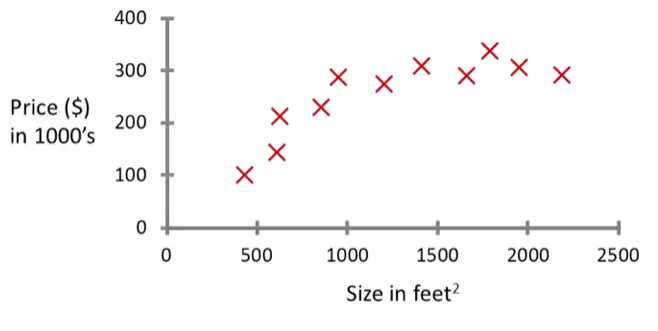
\includegraphics{img/sl1.png}

Here on the horizontal axis, the size of different houses in square
feet, and on the vertical axis, the price of different houses in
thousands of dollars.

So. Given this data, let's say we own a house that is, say 750 square
feet and hoping to sell the house and we want to know how much we can
get for the house.

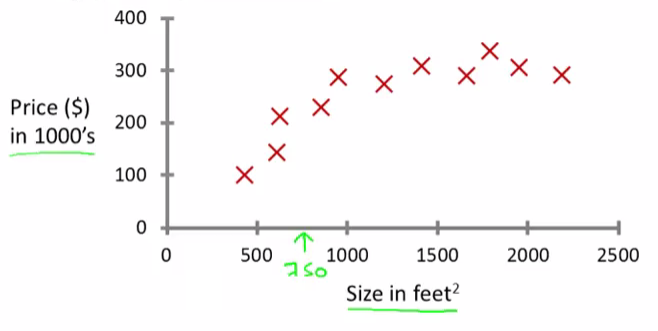
\includegraphics{img/sl2.png}

So how can the learning algorithm help?

One thing a learning algorithm might be able to do is put a straight
line through the data or to \textbf{``fit''} a straight line to the data
and, based on that, it looks like maybe the house can be sold for maybe
about \$150,000.

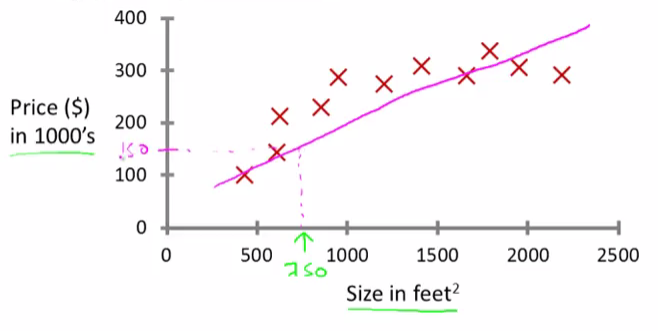
\includegraphics{img/sl3.png}

But maybe this isn't the only learning algorithm we can use. There might
be a better one. For example, instead of sending a straight line to the
data, we might decide that it's better to fit a \emph{quadratic
function} or a \emph{second-order polynomial} to this data.

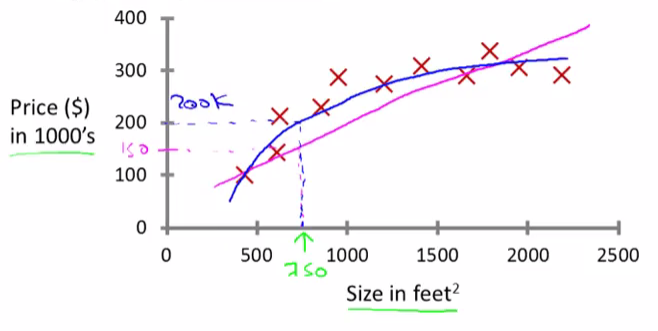
\includegraphics{img/sl4.png}

If we do that, and make a prediction here, then it looks like, well,
maybe we can sell the house for closer to \$200,000.

This is an example of a supervised learning algorithm.

The term supervised learning refers to the fact that we gave the
algorithm a data set in which the \textbf{``right answers''} were given.

The example above is also called a regression problem. A regression
problem is when we try to predict a \textbf{continuous} value output.
Namely the price in the example.

Here's another supervised learning example. Let's say we want to look at
medical records and try to predict of a breast cancer as malignant or
benign. If someone discovers a breast tumor, a lump in their breast, a
malignant tumor is a tumor that is harmful and dangerous and a benign
tumor is a tumor that is harmless. Let's see a collected data set and
suppose in the data set we have the size of the tumor on the horizontal
axis and on the vertical axis we plot one or zero, yes or no, whether or
not these are examples of tumors we've seen before are malignant (which
is one) or zero if not malignant or benign.

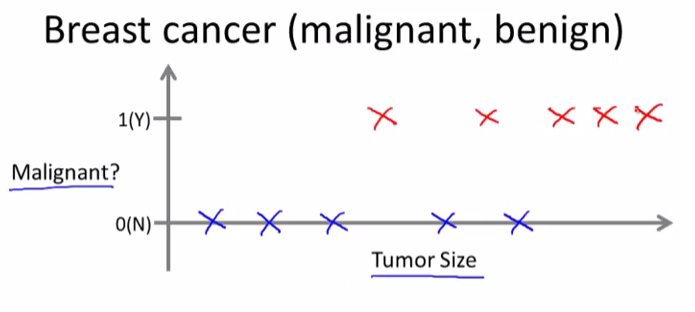
\includegraphics{img/sl5.png}

In this data set we have five examples of benign tumors, and five
examples of malignant tumors.

Let's say a person who tragically has a breast tumor, and let's say her
breast tumor size is known (rose arrow in the following figure).

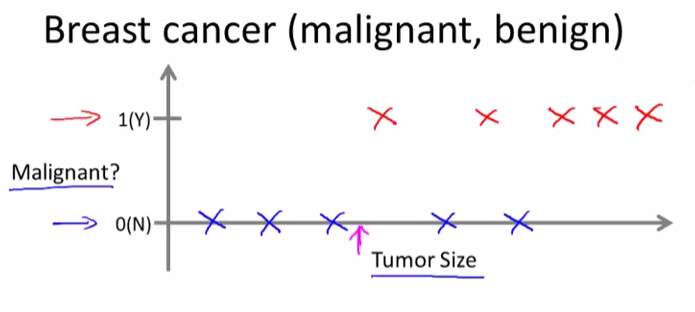
\includegraphics{img/sl6.png}

The machine learning question is, can you estimate what is the
probability that a tumor is malignant versus benign? To introduce a bit
more terminology this is an example of a \textbf{\emph{classification}}
problem.

The term classification refers to the fact that here we're trying to
predict a \textbf{discrete} value output: zero or one, malignant or
benign. And it turns out that in classification problems sometimes you
can have more than two values for the two possible values for the
output.

In classification problems there is another way to plot this data. Let's
use a slightly different set of symbols to plot this data. So if tumor
size is going to be the attribute that we are going to use to predict
malignancy or benignness, we can also draw the data like this.

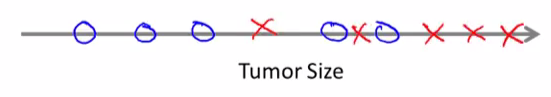
\includegraphics{img/sl7.png}

All we did was we took the data set on top and just mapped it down using
different symbols. So instead of drawing crosses, we are now going to
draw \texttt{O}'s for the benign tumors.

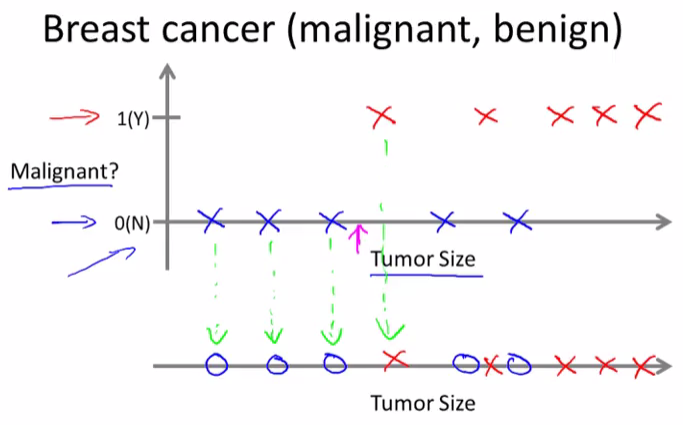
\includegraphics{img/sl8.png}

Now, in this example we use only one \textbf{feature} or one attribute,
mainly, the \emph{tumor size} in order to predict whether the tumor is
malignant or benign.

In other machine learning problems we may have more than one feature.

Here's an example. Let's say that instead of just knowing the tumor
size, we know both the age of the patients and the tumor size. In that
case maybe the data set will look like this.

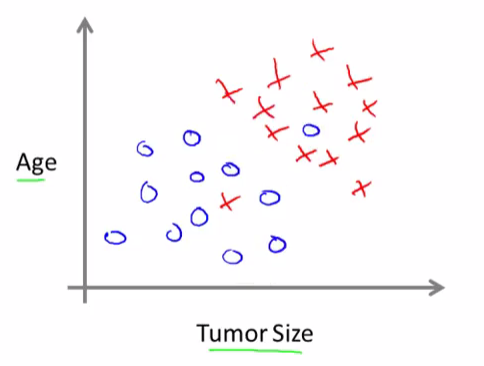
\includegraphics{img/sl9.png}

So, let's say a person who tragically has a tumor. And maybe, their
tumor size and age falls around there (rose point):

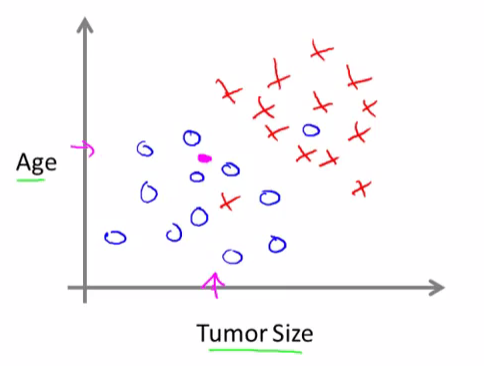
\includegraphics{img/sl10.png}

So given a data set like this, what the learning algorithm might do is
throw a straight line through the data to try to separate out the
malignant tumors from the benign ones. And with this, hopefully we can
decide that the person's tumor falls on this benign side and is
therefore more likely to be benign than malignant.

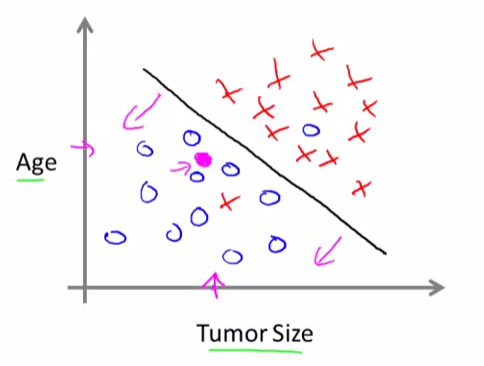
\includegraphics{img/sl11.png}

In this example we had \textbf{two features}, namely, the age of the
patient and the size of the tumor. In other machine learning problems we
will often have more features.

Most interesting learning algorithms is a learning algorithm that can
deal with, not just two or three or five features, but an
\textbf{infinite number of features}. So how do you deal with an
infinite number of features. How do you even store an infinite number of
things on the computer when your computer is gonna run out of memory.

\section*{Unsupervised Learning}\label{unsupervised-learning}
\addcontentsline{toc}{section}{Unsupervised Learning}

The second major type of machine learning problem is called Unsupervised
Learning.

The difference between Unsupervised Learning and Supervised Learning is
that in Supervised Learning we are told explicitly what is the so-called
right answers (data are labeled).

In Unsupervised Learning, we're given data that doesn't have any labels
or that all has the same label or really no labels. Like in this
example:

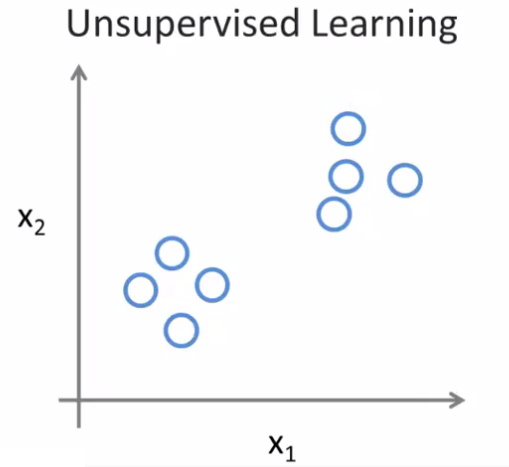
\includegraphics{img/ul1.png}

So we're given the data set and we're not told what to do with it and
we're not told what each data point is. Instead we're just told, here is
a data set. Can you find some structure in the data?

Given this data set, an Unsupervised Learning algorithm might decide
that the data lives in two different clusters.

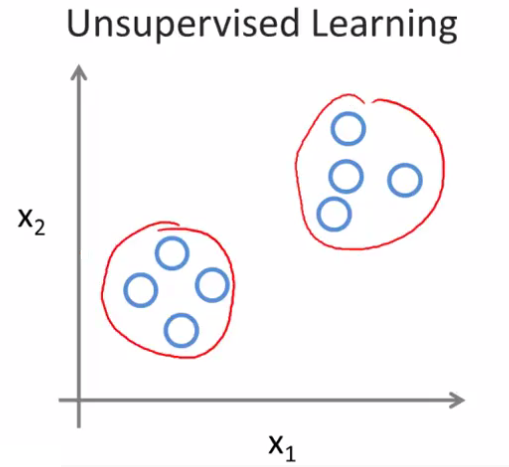
\includegraphics{img/ul2.png}

This is called a \textbf{clustering} algorithm.

Here are two examples where Unsupervised Learning or clustering is used.

Social network analysis:

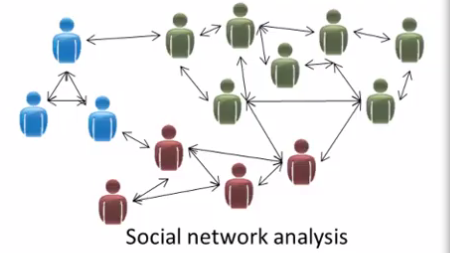
\includegraphics{img/ul3.png}

So given knowledge about which friends you email the most or given your
Facebook friends or your Google+ circles, can we automatically identify
which are cohesive groups of friends, also which are groups of people
that all know each other?

Market segmentation:

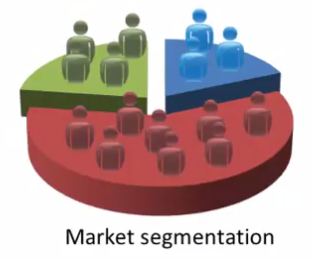
\includegraphics{img/ul4.png}

Many companies have huge databases of customer information. So, can you
look at this customer data set and automatically discover market
segments and automatically group your customers into different market
segments so that you can automatically and more efficiently sell or
market your different market segments together?

This is Unsupervised Learning because we have all this customer data,
but we don't know in advance what are the market segments and for the
customers in our data set, we don't know in advance who is in market
segment one, who is in market segment two, and so on. But we have to let
the algorithm discover all this just from the data.

◼

\part{Supervised Learning}\label{part-supervised-learning}
\addcontentsline{toc}{chapter}{(PART) Supervised Learning}

\part{Regression}\label{part-regression}
\addcontentsline{toc}{chapter}{(PART) Regression}

\chapter{Linear Regression}\label{linear-regression}

\section{Notation}\label{notation}

In general, we will let \(x_{ij}\) represent the value of the \(j\)th
variable for the \(i\)th observation, where \(i=1,2,\ldots,n\) and
\(j=1,2,\ldots,p\). We will use \(i\) to index the samples or
observations (from \(1\) tp \(n\)) and \(j\) will be used to index the
variables (or features) (from \(1\) to \(p\)). We let \(\textbf{X}\)
denote a \(n \times p\) matrix whose \((i,j)\)th element is \(x_{ij}\).
That is,

\[ \textbf{X}  = \begin{pmatrix}
    x_{11} & x_{12} & x_{13} & \dots  & x_{1p} \\
    x_{21} & x_{22} & x_{23} & \dots  & x_{2p} \\
    \vdots & \vdots & \vdots & \ddots & \vdots \\
    x_{n1} & x_{n2} & x_{n3} & \dots  & x_{np}
\end{pmatrix} \]

Note that it is useful to visualize \(\textbf{X}\) as a spreadsheet of
numbers with \(n\) rows and \(p\) columns. We will write the rows of
\(\textbf{X}\) as \(x_1 , x_2 , \ldots, x_n\). Here \(x_i\) is a vector
of length \(p\), containing the \(p\) variable measurements for the
\(i\)th observation. That is,

\[ x_i = \begin{pmatrix}
    x_{i1} \\
    x_{i2} \\
    \vdots \\
    x_{ip}
\end{pmatrix}\]

(Vectors are by default represented as columns.)

We will write the columns of \(\textbf{X}\) as
\(\textbf{x}_1 , \textbf{x}_2, \ldots, \textbf{x}_p\). Each is a vector
of length \(n\). That is,

\[ \textbf{x}_j = \begin{pmatrix}
    \textbf{x}_{1j} \\
    \textbf{x}_{2j} \\
    \vdots \\
    \textbf{x}_{nj}
\end{pmatrix}\]

Using this notation, the matrix \(\textbf{X}\) can be written as

\[ \textbf{X} = (\textbf{x}_1  \textbf{x}_2 \ldots \textbf{x}_p) \]

or

\[ \textbf{X} = \begin{pmatrix}
    x_{1}^T \\
    x_{2}^T \\
    \vdots \\
    x_{n}^T
\end{pmatrix}\]

The \(^T\) notation denotes the transpose of a matrix or vector.

We use \(y_i\) to denote the \(i\)th observation of the variable on
which we wish to make predictions. We write the set of all \(n\)
observations in vector form as

\[ \textbf{y} = \begin{pmatrix}
    y_{1}^T \\
    y_{2}^T \\
    \vdots \\
    y_{n}^T
\end{pmatrix}\]

Then the observed data consists of
\(\{(x_1, y_1), (x_2 , y_2 ), \ldots , (x_n , y_n )\}\), where each
\(x_i\) is a vector of length \(p\). (If \(p = 1\), then \(x_i\) is
simply a scalar).

\section{Model Representation}\label{model-representation}

Let's consider the example about predicting housing prices. We're going
to use this data set as an example,

\begin{figure}[htbp]
\centering
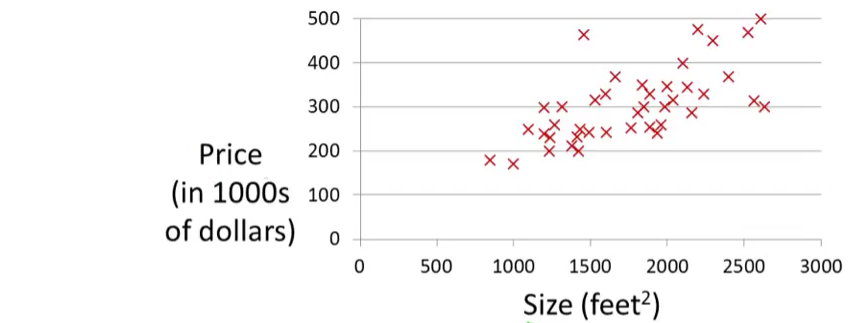
\includegraphics{img/mr1.png}
\caption{}
\end{figure}

Suppose that there is a person trying to sell a house of size 1250
square feet and he wants to know how much he might be able to sell the
house for. One thing we could do is fit a model. Maybe fit a straight
line to this data. Looks something like this,

\begin{figure}[htbp]
\centering
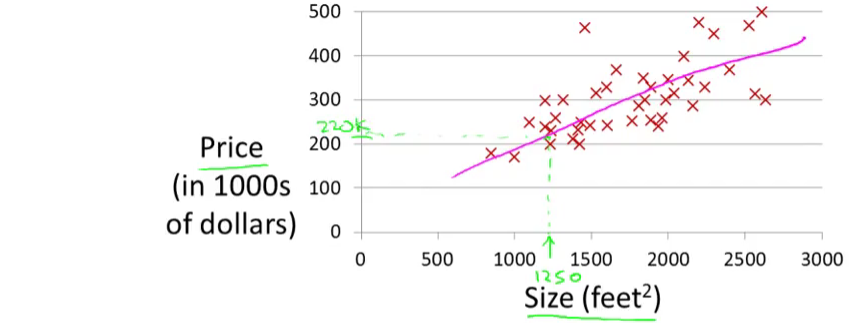
\includegraphics{img/mr2.png}
\caption{}
\end{figure}

and based on that, maybe he can sell the house for around \$220,000.
Recall that this is an example of a supervised learning algorithm. And
it's supervised learning because we're given the ``right answer'' for
each of our examples. More precisely, this is an example of a regression
problem where the term regression refers to the fact that we are
predicting a real-valued output namely the price.

More formally, in supervised learning, we have a data set and this data
set is called a \textbf{training set}. So for housing prices example, we
have a training set of different housing prices and our job is to learn
from this data how to predict prices of the houses.

Let's define some notation from this data set:

\begin{itemize}
\tightlist
\item
  The size of the house is the input variable.
\item
  The house price is the output variable.
\item
  The input variables are typically denoted using the variable symbol
  \(X\),
\item
  The inputs go by different names, such as \emph{predictors},
  \emph{independent variables}, \emph{features}, \emph{predictor} or
  sometimes just \emph{variables}.
\item
  The output variable is often called the \emph{response},
  \emph{dependent variable} or \emph{target}, and is typically denoted
  using the symbol \(Y\).
\item
  \((x_i,y_i)\) is the \(i\)th training example.
\item
  The set of \(\{(x_i, y_i)\}\) is the training set.
\item
  \(n\) is the number of training examples.
\end{itemize}

So here's how this supervised learning algorithm works. Suppose that we
observe a quantitative response \(Y\) and \(p\) different predictors,
\(X_1 , X_2 ,\ldots, X_p\) . We assume that there is some relationship
between \(Y\) and \(X = (X_1 , X_2 ,\ldots, X_p)\), which can be written
in the very general form

\[Y = f(X) + \epsilon\]

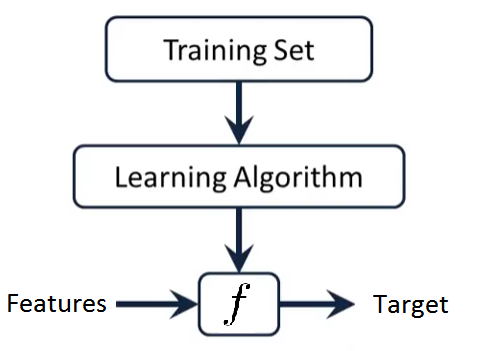
\includegraphics{img/mr3.png}

Here \(f\) is some fixed but unknown function of
\(X_1 , X_2 ,\ldots, X_p\) , and \(\epsilon\) is a random error term,
which is independent of \(X\) and has mean zero. The \(f\) function is
also called \emph{hypothesis} in Machine Learning. In general, the
function \(f\) may involve more than one input variable. In essence,
Supervised Learning refers to a set of approaches for estimating \(f\).

\section{\texorpdfstring{Why Estimate \(f\)
?}{Why Estimate f ?}}\label{why-estimate-f}

There are two main reasons that we may wish to estimate \(f\):
\emph{prediction} and \emph{inference}.

\subsection*{Prediction}\label{prediction}
\addcontentsline{toc}{subsection}{Prediction}

In many situations, a set of inputs \(X\) are readily available, but the
output \(Y\) cannot be easily obtained. In this setting, since the error
term averages to zero, we can predict \(Y\) using

\[ \hat{Y} = \hat{f}(X) \]

where \(\hat{f}\) represents our estimate for \(f\), and \(\hat{Y}\)
represents the resulting prediction for \(Y\). Like in the example above
about predicting housing prices.

We can measure the accuracy of \(\hat{Y}\) by using a \textbf{cost
function}. In the regression models, the most commonly-used measure is
the \emph{mean squared error} (MSE), given by

\[ MSE = \frac{1}{n} \sum_{i=1}^{n} (y_i - \hat{f}(x_i))^2\]

\subsection*{Inference}\label{inference}
\addcontentsline{toc}{subsection}{Inference}

We are often interested in understanding the way that \(Y\) is affected
as \(X_1 , X_2 ,\ldots, X_p\) change. In this situation we wish to
estimate \(f\) , but our goal is not necessarily to make predictions for
\(Y\). We instead want to understand the relationship between \(X\) and
\(Y\), or more specifically, to understand how \(Y\) changes as a
function of \(X_1 , X_2 ,\ldots, X_p\). In this case, one may be
interested in answering the following questions:

\begin{itemize}
\tightlist
\item
  Which predictors are associated with the response?
\item
  What is the relationship between the response and each predictor?
\item
  Can the relationship between Y and each predictor be adequately
  summarized using a linear equation, or is the relationship more
  complicated?
\end{itemize}

\section{Simple Linear Regression
Model}\label{simple-linear-regression-model}

\emph{Simple linear regression} is a very straightforward approach for
predicting a quantitative response \(Y\) on the basis of a single
predictor variable \(X\). It assumes that there is approximately a
linear relationship between \(X\) and \(Y\). Mathematically, we can
write this linear relationship as

\[ Y = \beta_0 + \beta_1 X + \epsilon \]
\[Y \approx \beta_0 + \beta_1 X\]

where \(\beta_0\) and \(\beta_1\) are two unknown constants that
represent the \emph{intercept} and \emph{slope}, also known as
\textbf{\emph{coefficients}} or \emph{parameters}, and \(\epsilon\) is
the error term.

Given some estimates \(\hat{\beta_0}\) and \(\hat{\beta_1}\) for the
model coefficients, we predict future inputs \(x\) using

\[\hat{y} = \hat{\beta_0} + \hat{\beta_1} x\]

where \(\hat{y}\) indicates a prediction of \(Y\) on the basis of
\(X = x\). The \emph{hat} symbol, \(\hat{}\), denotes an estimated
value.

\section{Estimating the Coefficients}\label{estimating-the-coefficients}

Let \(\hat{y}_i = \hat{\beta_0} + \hat{\beta_1} x_i\) be the prediction
for \(Y\) based on the \(i\)th value of \(X\). Then
\(e_i = y_i - \hat{y}_i\) represents the \(i\)th
\textbf{\emph{residual}}.

We define the \textbf{\emph{residual sum of squares}} (\textbf{RSS}) as

\[  \begin{aligned}
RSS &= e_1^2 + e_2^2 + \ldots + e_n^2 \\
    &= \sum_{i=1}^{n} e_i^2
 \end{aligned}  \]

or equivantly as

\[ \begin{aligned}
RSS &= (y_1 - \hat{\beta_0} - \hat{\beta_1} x_1)^2 + (y_2 - \hat{\beta_0} - \hat{\beta_1} x_2)^2 + \ldots + (y_n - \hat{\beta_0} - \hat{\beta_1} x_n)^2 \\
    &= \sum_{i=1}^{n} (y_i - \hat{\beta_0} - \hat{\beta_1} x_i)^2
\end{aligned} \]

The \emph{least squares} approach chooses \(\hat{\beta_0}\) and
\(\hat{\beta_1}\) to minimize the RSS. The minimizing values can be show
to be

\[  \begin{aligned}
\hat{\beta_1} &=  \frac{\sum_{i=1}^{n} (x_i - \bar{x})(y_i - \bar{y})  }{\sum_{i=1}^{n} (x_i - \bar{x})^2 } = \frac{s_{xy}}{s_x^2} \\
\text{and} \\
\hat{\beta_0} &= \bar{y} - \hat{\beta_1} \bar{x}
\end{aligned}  \]

where:

\begin{itemize}
\tightlist
\item
  \(\bar{x}=\frac{1}{n}\sum_{i=1}^nx_i\) is the \emph{sample mean}.
\item
  \(s_x^2=\frac{1}{n}\sum_{i=1}^n(x_i-\bar{x})^2\) is the \emph{sample
  variance}. The sample standard deviation is \(s_x=\sqrt{s_x^2}\).
\item
  \(s_{xy}=\frac{1}{n}\sum_{i=1}^n(x_i-\bar{x})(y_i-\bar{y})\) is the
  \emph{sample covariance}. It measures the degree of linear association
  between \(x_1,\ldots,x_n\) and \(y_1,\ldots,y_n\). Once scaled by
  \(s_xs_y\), it gives the \emph{sample correlation coefficient},
  \(r_{xy}=\frac{s_{xy}}{s_xs_y}\).
\end{itemize}

\begin{rmdinsight}
Click here to see the influence of the distance employed in the sum of
squares. Try to minimize the sum of squares for the different datasets.
The choices of intercept and slope that minimize the sum of squared
distances for a kind of distance are not the optimal for a different
kind of distance.
\end{rmdinsight}

\section{Assessing the Accuracy of the Coefficient
Estimates}\label{assessing-the-accuracy-of-the-coefficient-estimates}

The standard error of an estimator reflects how it varies under repeated
sampling. We have

\[ \text{SE}(\hat{\beta_1})^2 =  \frac{\sigma^2}{\sum_{i=1}^{n} (x_i - \bar{x})^2} \]

\[ \text{SE}(\hat{\beta_0})^2 = \sigma^2 \bigg[ \frac{1}{n} +  \frac{\bar{x}^2}{\sum_{i=1}^{n} (x_i - \bar{x})^2} \bigg] \]

where \(\sigma^2 = Var(\epsilon)\)

In general, \(\sigma^2\) is know known, but can be estimated from the
data. The estimate of \(\sigma\) is known as the \emph{residual standard
error}, and is given by

\[ \text{RSE} = \sqrt{\frac{\text{RSS}}{(n-2)}} \]

These standard errors can be used to compute \emph{confidence
intervals}. A \(95\%\) confidence interval is defined as a range of
values such that with \(95\%\) probability, the range will contain the
true unknown value of the parameter. It has the form

\[ \hat{\beta_1} \pm 2 \cdot \text{SE}(\hat{\beta_1}) \]

That is, there is approximately a \(95\%\) chance that the interval

\[ \bigg[  \hat{\beta_1} - 2 \cdot \text{SE}(\hat{\beta_1}), \hat{\beta_1} + 2 \cdot \text{SE}(\hat{\beta_1})   \bigg] \]

will contain the true value of \(\beta_1\). Similarly, a confidence
interval for \(\beta_0\) approximately takes the form

\[ \hat{\beta_0} \pm 2 \cdot \text{SE}(\hat{\beta_0}) \]

\subsection*{Hypothesis testing}\label{hypothesis-testing}
\addcontentsline{toc}{subsection}{Hypothesis testing}

Standard errors can also be used to perform \emph{hypothesis tests} on
the coefficients. The most common hypothesis test involves testing the
\emph{null hypothesis} of

\[ H_0 : \text{There is no relationship between} \, X \, \text{and} \, Y \]

versus the \emph{alternative hypothesis}

\[ H_1 : \text{There is some relationship between} \, X \, \text{and} \, Y \]

Mathematically, this corresponds to testing

\[ H_0 : \beta_1 = 0 \]

versus

\[ H_1 : \beta_1 \neq 0 \]

since if \(\beta_1 = 0\) then the simple linear regression model reduces
to \(Y = \beta_0 + \epsilon\), and \(X\) is not associated with \(Y\).

To test the null hypothesis \(H_0\), we compute a
\textbf{\emph{t-statistic}}, given by

\[ t = \frac{\hat{\beta_1} - 0}{\text{SE}(\hat{\beta_1})} \]

This will have a \(t\)-distribution (\emph{Student}) with \(n-2\)
degrees of freedom, assuming \(\beta_1=0\).

Using statistical software, it is easy to compute the probability of
observing any value equal to \(|t|\) or larger. We call this probability
the \textbf{\emph{p-value}}.

If p-value is small enough (typically under \(0.01\) (\(1\%\) error) or
\(0.05\) (\(5\%\) error)) we reject the null hypothesis, that is we
declare a relationship to exist between \(X\) and \(Y\).

\section{ANOVA and model fit}\label{anova-and-model-fit}

\subsection{ANOVA}\label{anova}

In this section we will see how the variance of \(Y\) is decomposed into
two parts, each one corresponding to the regression and to the error,
respectively. This decomposition is called the \emph{ANalysis Of
VAriance} (ANOVA).

Before explaining ANOVA, it is important to recall an interesting
result: \emph{the mean of the fitted values \(\hat Y_1,\ldots,\hat Y_n\)
is the mean of \(Y_1,\ldots, Y_n\)}. This is easily seen if we plug-in
the expression of \(\hat\beta_0\):

\begin{align*}
\frac{1}{n}\sum_{i=1}^n \hat Y_i=\frac{1}{n}\sum_{i=1}^n \left(\hat \beta_0+\hat\beta_1X_i\right)=\hat \beta_0+\hat\beta_1\bar X=\left(\bar Y - \hat\beta_1\bar X \right) + \hat\beta_1\bar X=\bar Y.
\end{align*}

The ANOVA decomposition considers the following measures of variation
related with the response:

\begin{itemize}
\tightlist
\item
  \(\text{SST}=\sum_{i=1}^n\left(Y_i-\bar Y\right)^2\), the
  \textbf{total sum of squares}. This is the \emph{total variation} of
  \(Y_1,\ldots,Y_n\), since \(\text{SST}=ns_y^2\), where \(s_y^2\) is
  the sample variance of \(Y_1,\ldots,Y_n\).
\item
  \(\text{SSR}=\sum_{i=1}^n\left(\hat Y_i-\bar Y\right)^2\), the
  \textbf{regression sum of squares}\footnote{Recall that SSR is
    different from RSS (Residual Sum of Squares}. This is the variation
  explained by the regression line, that is, \emph{the variation from
  \(\bar Y\) that is explained by the estimated conditional mean
  \(\hat Y_i=\hat\beta_0+\hat\beta_1X_i\)}.
  \(\text{SSR}=ns_{\hat y}^2\), where \(s_{\hat y}^2\) is the sample
  variance of \(\hat Y_1,\ldots,\hat Y_n\).
\item
  \(\text{SSE}=\sum_{i=1}^n\left(Y_i-\hat Y_i\right)^2\), the
  \textbf{sum of squared errors}\footnote{Recall that SSE and RSS (for
    \((\hat \beta_0,\hat \beta_1)\)) are just different names for
    referring to the same quantity:
    \(\text{SSE}=\sum_{i=1}^n\left(Y_i-\hat Y_i\right)^2=\sum_{i=1}^n\left(Y_i-\hat \beta_0-\hat \beta_1X_i\right)^2=\mathrm{RSS}\left(\hat \beta_0,\hat \beta_1\right)\).}.
  Is the variation around the conditional mean. Recall that
  \(\text{SSE}=\sum_{i=1}^n \hat\varepsilon_i^2=(n-2)\hat\sigma^2\),
  where \(\hat\sigma^2\) is the sample variance of
  \(\hat \varepsilon_1,\ldots,\hat \varepsilon_n\).
\end{itemize}

The ANOVA decomposition is

\begin{align*}
\underbrace{\text{SST}}_{\text{Variation of }Y_i's} = \underbrace{\text{SSR}}_{\text{Variation of }\hat Y_i's} + \underbrace{\text{SSE}}_{\text{Variation of }\hat \varepsilon_i's}
\end{align*}

The graphical interpretation of this equation is shown in the following
figures.

\begin{figure}

{\centering 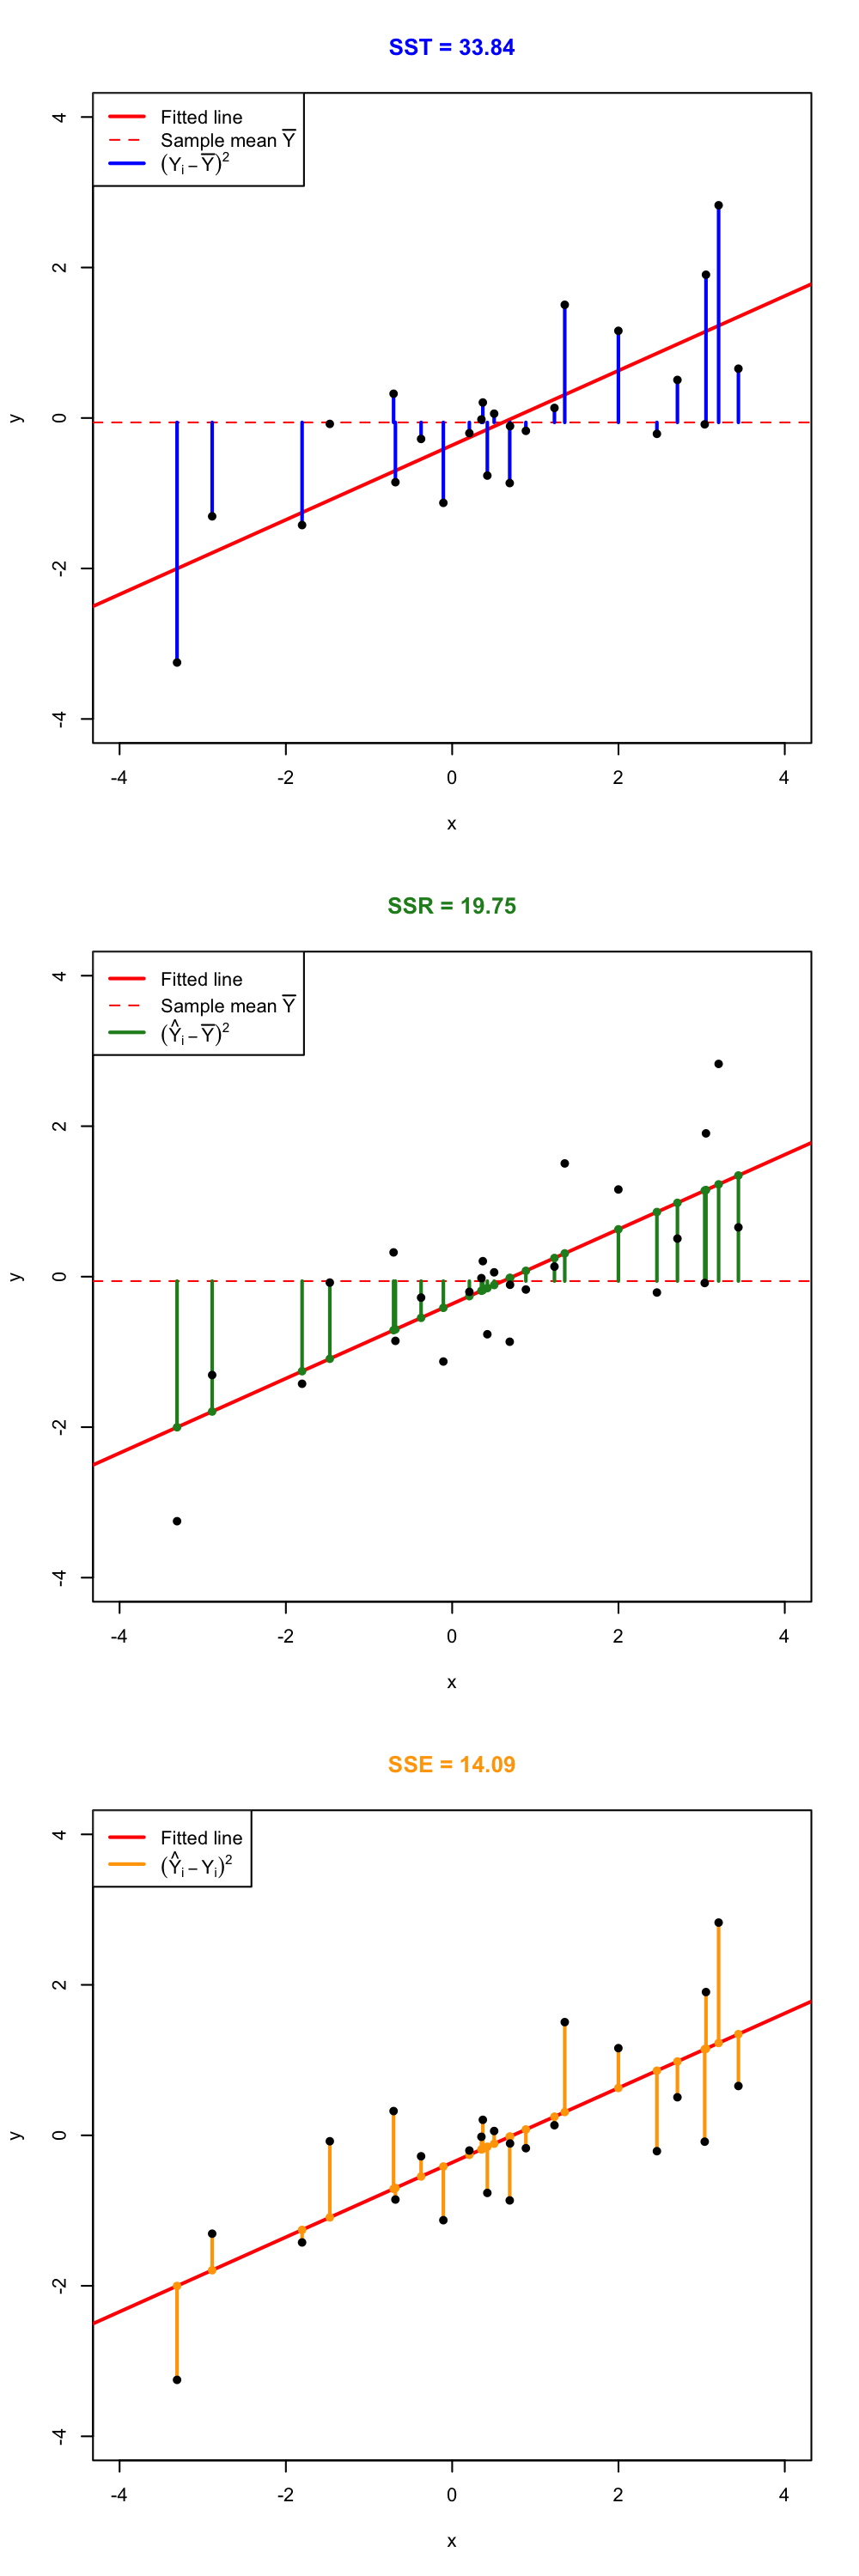
\includegraphics[width=0.7\linewidth]{img/anova} 

}

\caption{Visualization of the ANOVA decomposition. SST measures the variation of $Y_1,\ldots,Y_n$ with respect to $\bar Y$. SST measures the variation with respect to the conditional means, $\hat \beta_0+\hat\beta_1X_i$. SSE collects the variation of the residuals.}\label{fig:anova}
\end{figure}

\begin{rmdinsight}
Click here to see the ANOVA decomposition and its dependence on
\(\sigma^2\) and \(\hat\sigma^2\).'
\end{rmdinsight}

The ANOVA table summarizes the decomposition of the variance. Here is
given in the layout employed by \texttt{R}.

\begin{longtable}[]{@{}llllll@{}}
\toprule
& Degrees of freedom & Sum Squares & Mean Squares & \(F\)-value &
\(p\)-value\tabularnewline
\midrule
\endhead
Predictor & \(1\) & SSR & \(\frac{\text{SSR}}{1}\) &
\(\frac{\text{SSR}/1}{\text{SSE}/(n-2)}\) & \(p\)\tabularnewline
Residuals & \(n - 2\) & SSE & \(\frac{\text{SSE}}{n-2}\) &
&\tabularnewline
\bottomrule
\end{longtable}

The \texttt{anova} function in \texttt{R} takes a model as an input and
returns the ANOVA table.

The ``\(F\)-value'' of the ANOVA table represents the value of the
\(F\)-statistic \(\frac{\text{SSR}/1}{\text{SSE}/(n-2)}\). This
statistic is employed to test

\begin{align*}
H_0:\beta_1=0\quad\text{vs.}\quad H_1:\beta_1\neq 0,
\end{align*}

that is, the hypothesis of no linear dependence of \(Y\) on \(X\). The
result of this test is completely equivalent to the \(t\)-test for
\(\beta_1\) that we saw previously in the Hypothesis testing (this is
something \emph{specific for simple linear regression} -- the \(F\)-test
will not be equivalent to the \(t\)-test for \(\beta_1\) in the Mulitple
Linear Regression).

It happens that

\begin{align*}
F=\frac{\text{SSR}/1}{\text{SSE}/(n-2)}\stackrel{H_0}{\sim} F_{1,n-2},
\end{align*}

where \(F_{1,n-2}\) is the \emph{Snedecor's \(F\)
distribution}\footnote{The \(F_{n,m}\) distribution arises as the
  quotient of two independent random variables \(\chi^2_n\) and
  \(\chi^2_m\), \(\frac{\chi^2_n/n}{\chi^2_m/m}\).} with \(1\) and
\(n-2\) degrees of freedom.

If \(H_0\) is true, then \(F\) is expected to be \emph{small} since SSR
will be close to zero. The \(p\)-value of this test is the same as the
\(p\)-value of the \(t\)-test for \(H_0:\beta_1=0\).

\subsection{\texorpdfstring{The \(R^2\)
Statistic}{The R\^{}2 Statistic}}\label{the-r2-statistic}

To calculate \(R^2\), we use the formula

\[ R^2 = \frac{\text{TSS} - \text{RSS}}{\text{TSS}} = 1- \frac{\text{RSS}}{\text{TSS}} \]

where \(\text{TSS} = \sum (y_i - \bar{y})^2\) is the \emph{total sum of
squared}.

\(R^2\) measures the \emph{proportion of variability in} \(Y\)
\emph{that can be explained using} \(X\). An \(R^2\) statistic that is
close to 1 indicates that a large proportion of the variability in the
response has been explained by the regression. A number near 0 indicates
that the regression did not explain much of the variability in the
response; this might occur because the linear model is wrong, or the
inherent error \(\sigma^2\) is high, or both.

It can be shown that in this simple linear linear regression setting
that \(R^2 = r^2\), where \(r\) is the correlation between \(X\) and
\(Y\):

\[ r = \frac{cov(X,Y)}{\sigma_X \sigma_Y} \]

\begin{rmdcaution}
\(R^2\) does not measure the correctness of a linear model but its
\textbf{usefulness} (for prediction, for \emph{explaining the variance}
of \(Y\)), assuming the model is correct.

Trusting blindly the \(R^2\) can lead to catastrophic conclusions, since
the model may not be correct.
\end{rmdcaution}

So remember:

\begin{rmdinsight}
A large \(R^2\) means \emph{nothing} if the \textbf{assumptions of the
model do not hold}. \(R^2\) is the proportion of variance of \(Y\)
explained by \(X\), but, of course, \emph{only when the linear model is
correct}.
\end{rmdinsight}

◼

\chapter*{PW 1}\label{pw-1}
\addcontentsline{toc}{chapter}{PW 1}

\section{\texorpdfstring{Some \texttt{R}
basics}{Some R basics}}\label{some-r-basics}

\subsection{Basic Commands}\label{basic-commands}

\texttt{R} uses functions to perform operations. To run a function
called \texttt{funcname},we type \texttt{funcname(input1,\ input2)} ,
where the inputs (or arguments) \texttt{input1} and \texttt{input2} tell
\texttt{R} how to run the function. A function can have any number of
inputs. For example, to create a vector of numbers, we use the function
\texttt{c()} (for \emph{concatenate}).

\begin{Shaded}
\begin{Highlighting}[]
\NormalTok{x <-}\StringTok{ }\KeywordTok{c}\NormalTok{(}\DecValTok{1}\NormalTok{,}\DecValTok{3}\NormalTok{,}\DecValTok{2}\NormalTok{,}\DecValTok{5}\NormalTok{)}
\NormalTok{x}
\CommentTok{#ans> [1] 1 3 2 5}
\end{Highlighting}
\end{Shaded}

Note that the \texttt{\textgreater{}} is not part of the command;
rather, it is printed by \texttt{R} to indicate that it is ready for
another command to be entered. We can also save things using \texttt{=}
rather than \texttt{\textless{}-}. Note that the answer in the code
above is followed by \texttt{\#ans\textgreater{}} while in the
\texttt{R} console it is not.

\begin{Shaded}
\begin{Highlighting}[]
\NormalTok{x =}\StringTok{ }\KeywordTok{c}\NormalTok{(}\DecValTok{1}\NormalTok{,}\DecValTok{6}\NormalTok{,}\DecValTok{2}\NormalTok{)}
\NormalTok{x}
\CommentTok{#ans> [1] 1 6 2}
\NormalTok{y =}\StringTok{ }\KeywordTok{c}\NormalTok{(}\DecValTok{1}\NormalTok{,}\DecValTok{4}\NormalTok{,}\DecValTok{3}\NormalTok{)}
\KeywordTok{length}\NormalTok{(x)}
\CommentTok{#ans> [1] 3}
\KeywordTok{length}\NormalTok{(y)}
\CommentTok{#ans> [1] 3}
\NormalTok{x+y}
\CommentTok{#ans> [1]  2 10  5}
\end{Highlighting}
\end{Shaded}

Hitting the \emph{up arrow} multiple times will display the previous
commands, which can then be edited. This is useful since one often
wishes to repeat a similar command.

The \texttt{ls()} function allows us to look at a list of all of the
objects, such \texttt{ls()} as data and functions, that we have saved so
far. The \texttt{rm()} function can be used to delete any object that we
don't want.

\begin{Shaded}
\begin{Highlighting}[]
\KeywordTok{ls}\NormalTok{()}
\CommentTok{#ans> [1] "x" "y"}
\KeywordTok{rm}\NormalTok{(x)}
\KeywordTok{ls}\NormalTok{()}
\CommentTok{#ans> [1] "y"}
\end{Highlighting}
\end{Shaded}

\subsection{Vectors}\label{vectors}

\begin{Shaded}
\begin{Highlighting}[]

\CommentTok{# A handy way of creating sequences is the operator :}
\CommentTok{# Sequence from 1 to 5}
\DecValTok{1}\NormalTok{:}\DecValTok{5}
\CommentTok{#ans> [1] 1 2 3 4 5}

\CommentTok{# Storing some vectors}
\NormalTok{vec <-}\StringTok{ }\KeywordTok{c}\NormalTok{(-}\FloatTok{4.12}\NormalTok{, }\DecValTok{0}\NormalTok{, }\FloatTok{1.1}\NormalTok{, }\DecValTok{1}\NormalTok{, }\DecValTok{3}\NormalTok{, }\DecValTok{4}\NormalTok{)}
\NormalTok{vec}
\CommentTok{#ans> [1] -4.12  0.00  1.10  1.00  3.00  4.00}

\CommentTok{# Entry-wise operations}
\NormalTok{vec +}\StringTok{ }\DecValTok{1}
\CommentTok{#ans> [1] -3.12  1.00  2.10  2.00  4.00  5.00}
\NormalTok{vec^}\DecValTok{2}
\CommentTok{#ans> [1] 16.97  0.00  1.21  1.00  9.00 16.00}

\CommentTok{# If you want to access a position of a vector, use [position]}
\NormalTok{vec[}\DecValTok{6}\NormalTok{]}
\CommentTok{#ans> [1] 4}

\CommentTok{# You also can change elements}
\NormalTok{vec[}\DecValTok{2}\NormalTok{] <-}\StringTok{ }\NormalTok{-}\DecValTok{1}
\NormalTok{vec}
\CommentTok{#ans> [1] -4.12 -1.00  1.10  1.00  3.00  4.00}

\CommentTok{# If you want to access all the elements except a position, use [-position]}
\NormalTok{vec[-}\DecValTok{2}\NormalTok{]}
\CommentTok{#ans> [1] -4.12  1.10  1.00  3.00  4.00}

\CommentTok{# Also with vectors as indexes}
\NormalTok{vec[}\DecValTok{1}\NormalTok{:}\DecValTok{2}\NormalTok{]}
\CommentTok{#ans> [1] -4.12 -1.00}

\CommentTok{# And also}
\NormalTok{vec[-}\KeywordTok{c}\NormalTok{(}\DecValTok{1}\NormalTok{, }\DecValTok{2}\NormalTok{)]}
\CommentTok{#ans> [1] 1.1 1.0 3.0 4.0}
\end{Highlighting}
\end{Shaded}

\begin{rmdexercise}
Do the following:

\begin{itemize}
\tightlist
\item
  Create the vector \(x=(1, 7, 3, 4)\).
\item
  Create the vector \(y=(100, 99, 98, ..., 2, 1)\).
\item
  Compute \(x_3+y_4\) and \(\cos(x_3) + \sin(x_2) e^{-y_2}\). (Answers:
  \texttt{100}, \texttt{-0.9899925})
\item
  Set \(x_{3}=0\) and \(y_{2}=-1\). Recompute the previous expressions.
  (Answers: \texttt{97}, \texttt{2.785875})
\item
  Index \(y\) by \(x+1\) and store it as \texttt{z}. What is the output?
  (Answer: \texttt{z} is \texttt{c(-1,\ 93,\ 100,\ 96)})
\end{itemize}
\end{rmdexercise}

\subsection{Matrices, data frames and
lists}\label{matrices-data-frames-and-lists}

\begin{Shaded}
\begin{Highlighting}[]
\CommentTok{# A matrix is an array of vectors}
\NormalTok{A <-}\StringTok{ }\KeywordTok{matrix}\NormalTok{(}\DecValTok{1}\NormalTok{:}\DecValTok{4}\NormalTok{, }\DataTypeTok{nrow =} \DecValTok{2}\NormalTok{, }\DataTypeTok{ncol =} \DecValTok{2}\NormalTok{)}
\NormalTok{A}
\CommentTok{#ans>      [,1] [,2]}
\CommentTok{#ans> [1,]    1    3}
\CommentTok{#ans> [2,]    2    4}

\CommentTok{# Another matrix}
\NormalTok{B <-}\StringTok{ }\KeywordTok{matrix}\NormalTok{(}\DecValTok{1}\NormalTok{:}\DecValTok{4}\NormalTok{, }\DataTypeTok{nrow =} \DecValTok{2}\NormalTok{, }\DataTypeTok{ncol =} \DecValTok{2}\NormalTok{, }\DataTypeTok{byrow =} \OtherTok{TRUE}\NormalTok{)}
\NormalTok{B}
\CommentTok{#ans>      [,1] [,2]}
\CommentTok{#ans> [1,]    1    2}
\CommentTok{#ans> [2,]    3    4}

\CommentTok{# Binding by rows or columns}
\KeywordTok{rbind}\NormalTok{(}\DecValTok{1}\NormalTok{:}\DecValTok{3}\NormalTok{, }\DecValTok{4}\NormalTok{:}\DecValTok{6}\NormalTok{)}
\CommentTok{#ans>      [,1] [,2] [,3]}
\CommentTok{#ans> [1,]    1    2    3}
\CommentTok{#ans> [2,]    4    5    6}
\KeywordTok{cbind}\NormalTok{(}\DecValTok{1}\NormalTok{:}\DecValTok{3}\NormalTok{, }\DecValTok{4}\NormalTok{:}\DecValTok{6}\NormalTok{)}
\CommentTok{#ans>      [,1] [,2]}
\CommentTok{#ans> [1,]    1    4}
\CommentTok{#ans> [2,]    2    5}
\CommentTok{#ans> [3,]    3    6}

\CommentTok{# Entry-wise operations}
\NormalTok{A +}\StringTok{ }\DecValTok{1}
\CommentTok{#ans>      [,1] [,2]}
\CommentTok{#ans> [1,]    2    4}
\CommentTok{#ans> [2,]    3    5}
\NormalTok{A *}\StringTok{ }\NormalTok{B}
\CommentTok{#ans>      [,1] [,2]}
\CommentTok{#ans> [1,]    1    6}
\CommentTok{#ans> [2,]    6   16}

\CommentTok{# Accessing elements}
\NormalTok{A[}\DecValTok{2}\NormalTok{, }\DecValTok{1}\NormalTok{] }\CommentTok{# Element (2, 1)}
\CommentTok{#ans> [1] 2}
\NormalTok{A[}\DecValTok{1}\NormalTok{, ] }\CommentTok{# First row}
\CommentTok{#ans> [1] 1 3}
\NormalTok{A[, }\DecValTok{2}\NormalTok{] }\CommentTok{# First column}
\CommentTok{#ans> [1] 3 4}

\CommentTok{# A data frame is a matrix with column names}
\CommentTok{# Useful when you have multiple variables}
\NormalTok{myDf <-}\StringTok{ }\KeywordTok{data.frame}\NormalTok{(}\DataTypeTok{var1 =} \DecValTok{1}\NormalTok{:}\DecValTok{2}\NormalTok{, }\DataTypeTok{var2 =} \DecValTok{3}\NormalTok{:}\DecValTok{4}\NormalTok{)}
\NormalTok{myDf}
\CommentTok{#ans>   var1 var2}
\CommentTok{#ans> 1    1    3}
\CommentTok{#ans> 2    2    4}

\CommentTok{# You can change names}
\KeywordTok{names}\NormalTok{(myDf) <-}\StringTok{ }\KeywordTok{c}\NormalTok{(}\StringTok{"newname1"}\NormalTok{, }\StringTok{"newname2"}\NormalTok{)}
\NormalTok{myDf}
\CommentTok{#ans>   newname1 newname2}
\CommentTok{#ans> 1        1        3}
\CommentTok{#ans> 2        2        4}

\CommentTok{# The nice thing is that you can access variables by its name with the $ operator}
\NormalTok{myDf$newname1}
\CommentTok{#ans> [1] 1 2}

\CommentTok{# And create new variables also (it has to be of the same}
\CommentTok{# length as the rest of variables)}
\NormalTok{myDf$myNewVariable <-}\StringTok{ }\KeywordTok{c}\NormalTok{(}\DecValTok{0}\NormalTok{, }\DecValTok{1}\NormalTok{)}
\NormalTok{myDf}
\CommentTok{#ans>   newname1 newname2 myNewVariable}
\CommentTok{#ans> 1        1        3             0}
\CommentTok{#ans> 2        2        4             1}

\CommentTok{# A list is a collection of arbitrary variables}
\NormalTok{myList <-}\StringTok{ }\KeywordTok{list}\NormalTok{(}\DataTypeTok{vec =} \NormalTok{vec, }\DataTypeTok{A =} \NormalTok{A, }\DataTypeTok{myDf =} \NormalTok{myDf)}

\CommentTok{# Access elements by names}
\NormalTok{myList$vec}
\CommentTok{#ans> [1] -4.12 -1.00  1.10  1.00  3.00  4.00}
\NormalTok{myList$A}
\CommentTok{#ans>      [,1] [,2]}
\CommentTok{#ans> [1,]    1    3}
\CommentTok{#ans> [2,]    2    4}
\NormalTok{myList$myDf}
\CommentTok{#ans>   newname1 newname2 myNewVariable}
\CommentTok{#ans> 1        1        3             0}
\CommentTok{#ans> 2        2        4             1}

\CommentTok{# Reveal the structure of an object}
\KeywordTok{str}\NormalTok{(myList)}
\CommentTok{#ans> List of 3}
\CommentTok{#ans>  $ vec : num [1:6] -4.12 -1 1.1 1 3 4}
\CommentTok{#ans>  $ A   : int [1:2, 1:2] 1 2 3 4}
\CommentTok{#ans>  $ myDf:'data.frame': 2 obs. of  3 variables:}
\CommentTok{#ans>   ..$ newname1     : int [1:2] 1 2}
\CommentTok{#ans>   ..$ newname2     : int [1:2] 3 4}
\CommentTok{#ans>   ..$ myNewVariable: num [1:2] 0 1}
\KeywordTok{str}\NormalTok{(myDf)}
\CommentTok{#ans> 'data.frame': 2 obs. of  3 variables:}
\CommentTok{#ans>  $ newname1     : int  1 2}
\CommentTok{#ans>  $ newname2     : int  3 4}
\CommentTok{#ans>  $ myNewVariable: num  0 1}

\CommentTok{# A less lengthy output}
\KeywordTok{names}\NormalTok{(myList)}
\CommentTok{#ans> [1] "vec"  "A"    "myDf"}
\end{Highlighting}
\end{Shaded}

\subsection{Graphics}\label{graphics}

The \texttt{plot()} function is the primary way to plot data in
\texttt{R} . For instance, \texttt{plot(x,y)} produces a scatterplot of
the numbers in \texttt{x} versus the numbers in \texttt{y}. There are
many additional options that can be passed in to the \texttt{plot()}
function. For example, passing in the argument \texttt{xlab} will result
in a label on the \texttt{x-axis}. To find out more information about
the \texttt{plot()} function, type \texttt{?plot}.

\begin{Shaded}
\begin{Highlighting}[]
\NormalTok{x=}\KeywordTok{rnorm}\NormalTok{(}\DecValTok{100}\NormalTok{)}
\CommentTok{# The rnorm() function generates a vector of random normal variables,}
\CommentTok{# rnorm() with first argument n the sample size. Each time we call this}
\CommentTok{# function, we will get a different answer.}
\NormalTok{y=}\KeywordTok{rnorm}\NormalTok{(}\DecValTok{100}\NormalTok{)}
\KeywordTok{plot}\NormalTok{(x,y)}
\end{Highlighting}
\end{Shaded}

\begin{center}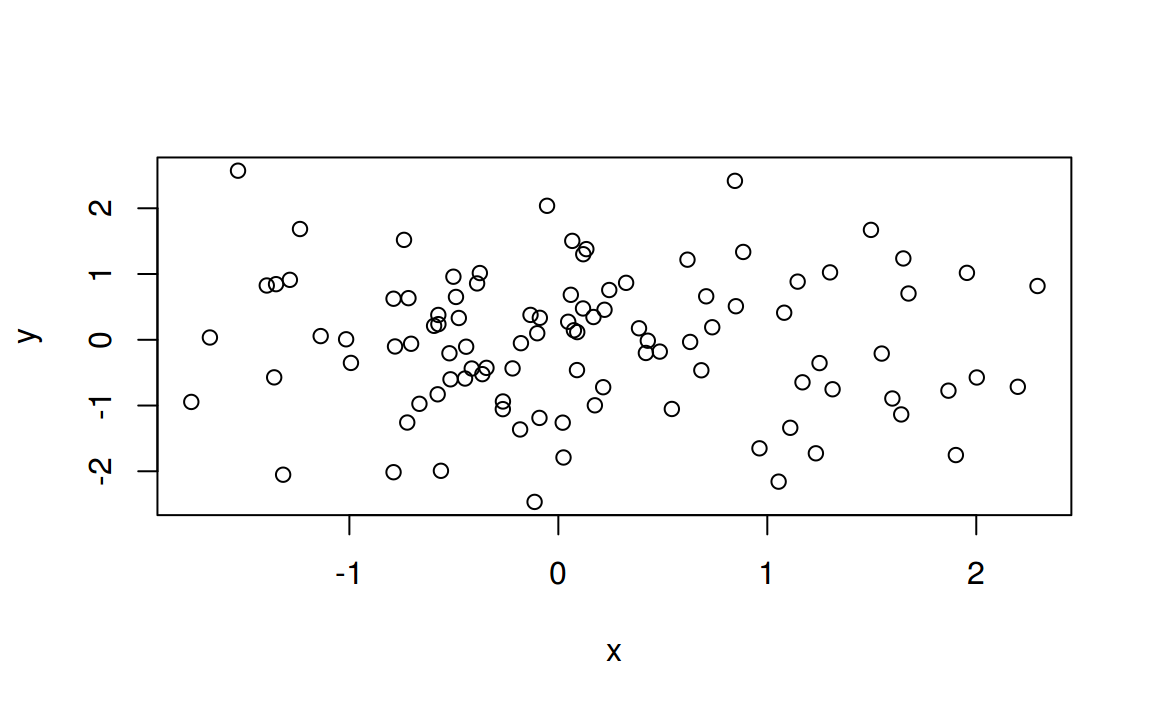
\includegraphics[width=0.7\linewidth]{Machine-Learning_files/figure-latex/unnamed-chunk-15-1} \end{center}

\begin{Shaded}
\begin{Highlighting}[]

\CommentTok{# with titles}
\KeywordTok{plot}\NormalTok{(x,y,}\DataTypeTok{xlab=}\StringTok{"this is the x-axis"}\NormalTok{,}\DataTypeTok{ylab=}\StringTok{"this is the y-axis"}\NormalTok{,}
\DataTypeTok{main=}\StringTok{"Plot of X vs Y"}\NormalTok{)}
\end{Highlighting}
\end{Shaded}

\begin{center}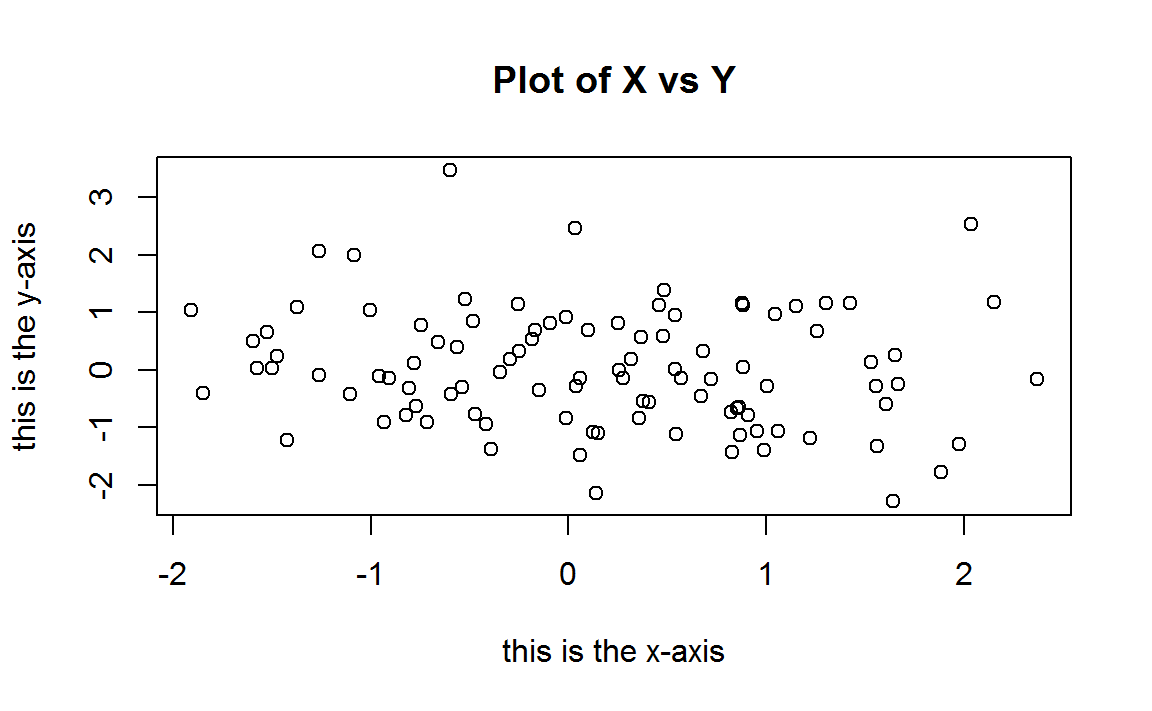
\includegraphics[width=0.7\linewidth]{Machine-Learning_files/figure-latex/unnamed-chunk-15-2} \end{center}

\subsection{Distributions}\label{distributions}

\begin{Shaded}
\begin{Highlighting}[]
\CommentTok{# R allows to sample [r], compute density/probability mass [d],}
\CommentTok{# compute distribution function [p] and compute quantiles [q] for several}
\CommentTok{# continuous and discrete distributions. The format employed is [rdpq]name,}
\CommentTok{# where name stands for:}
\CommentTok{# - norm -> Normal}
\CommentTok{# - unif -> Uniform}
\CommentTok{# - exp -> Exponential}
\CommentTok{# - t -> Student's t}
\CommentTok{# - f -> Snedecor's F (Fisher)}
\CommentTok{# - chisq -> Chi squared}
\CommentTok{# - pois -> Poisson}
\CommentTok{# - binom -> Binomial}
\CommentTok{# More distributions: ?Distributions}


\CommentTok{# Sampling from a Normal - 100 random points from a N(0, 1)}
\KeywordTok{rnorm}\NormalTok{(}\DataTypeTok{n =} \DecValTok{10}\NormalTok{, }\DataTypeTok{mean =} \DecValTok{0}\NormalTok{, }\DataTypeTok{sd =} \DecValTok{1}\NormalTok{)}
\CommentTok{#ans>  [1] -0.53758  1.06981 -0.86083 -0.44062  1.57230 -0.00322  1.66986}
\CommentTok{#ans>  [8] -0.65939  0.40302 -0.84128}

\CommentTok{# If you want to have always the same result, set the seed of the random number}
\CommentTok{# generator}
\KeywordTok{set.seed}\NormalTok{(}\DecValTok{45678}\NormalTok{)}
\KeywordTok{rnorm}\NormalTok{(}\DataTypeTok{n =} \DecValTok{10}\NormalTok{, }\DataTypeTok{mean =} \DecValTok{0}\NormalTok{, }\DataTypeTok{sd =} \DecValTok{1}\NormalTok{)}
\CommentTok{#ans>  [1]  1.440 -0.720  0.671 -0.422  0.378 -1.667 -0.508  0.443 -1.799 -0.618}

\CommentTok{# Plotting the density of a N(0, 1) - the Gauss bell}
\NormalTok{x <-}\StringTok{ }\KeywordTok{seq}\NormalTok{(-}\DecValTok{4}\NormalTok{, }\DecValTok{4}\NormalTok{, }\DataTypeTok{l =} \DecValTok{100}\NormalTok{)}
\NormalTok{y <-}\StringTok{ }\KeywordTok{dnorm}\NormalTok{(}\DataTypeTok{x =} \NormalTok{x, }\DataTypeTok{mean =} \DecValTok{0}\NormalTok{, }\DataTypeTok{sd =} \DecValTok{1}\NormalTok{)}
\KeywordTok{plot}\NormalTok{(x, y, }\DataTypeTok{type =} \StringTok{"l"}\NormalTok{)}
\end{Highlighting}
\end{Shaded}

\begin{center}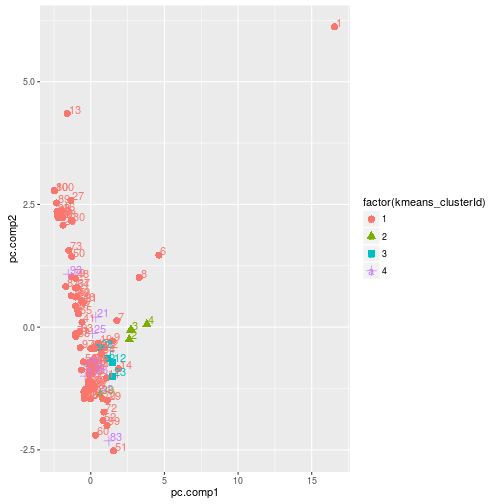
\includegraphics[width=0.7\linewidth]{Machine-Learning_files/figure-latex/unnamed-chunk-16-1} \end{center}

\begin{Shaded}
\begin{Highlighting}[]

\CommentTok{# Plotting the distribution function of a N(0, 1)}
\NormalTok{x <-}\StringTok{ }\KeywordTok{seq}\NormalTok{(-}\DecValTok{4}\NormalTok{, }\DecValTok{4}\NormalTok{, }\DataTypeTok{l =} \DecValTok{100}\NormalTok{)}
\NormalTok{y <-}\StringTok{ }\KeywordTok{pnorm}\NormalTok{(}\DataTypeTok{q =} \NormalTok{x, }\DataTypeTok{mean =} \DecValTok{0}\NormalTok{, }\DataTypeTok{sd =} \DecValTok{1}\NormalTok{)}
\KeywordTok{plot}\NormalTok{(x, y, }\DataTypeTok{type =} \StringTok{"l"}\NormalTok{, }\DataTypeTok{lwd =} \DecValTok{3}\NormalTok{, }\DataTypeTok{main=}\StringTok{"The distribution function of a N(0, 1)"}\NormalTok{)}
\end{Highlighting}
\end{Shaded}

\begin{center}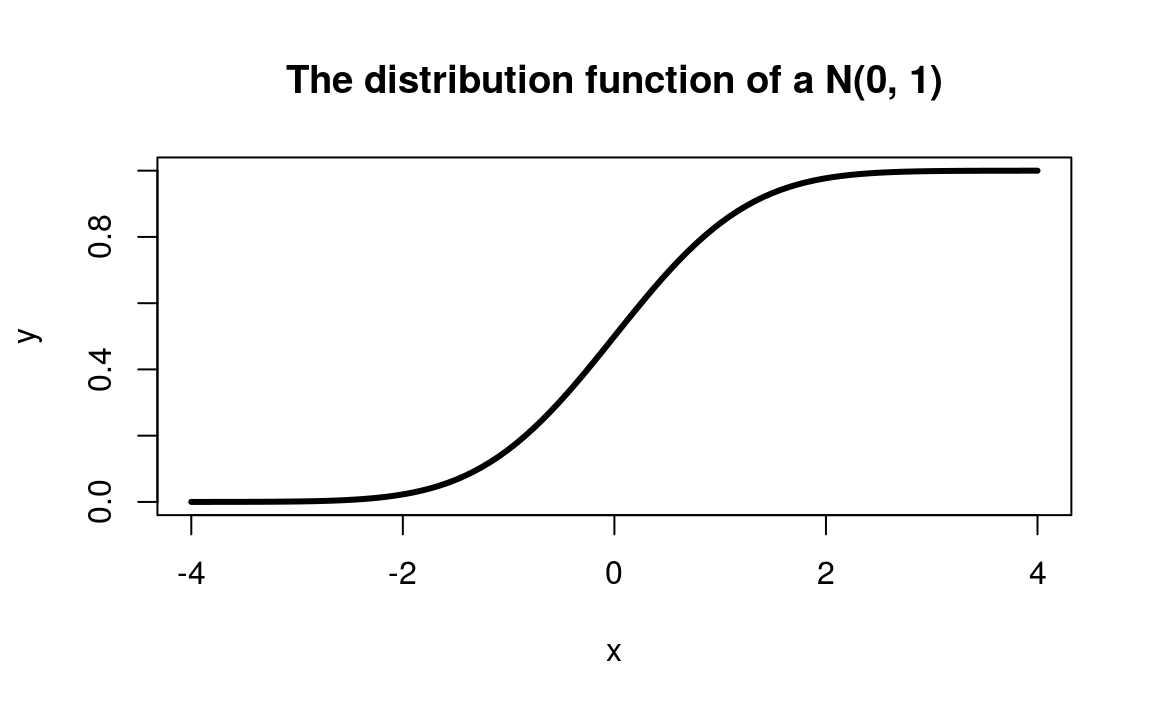
\includegraphics[width=0.7\linewidth]{Machine-Learning_files/figure-latex/unnamed-chunk-16-2} \end{center}

\begin{Shaded}
\begin{Highlighting}[]

\CommentTok{# Computing the 95% quantile for a N(0, 1)}
\KeywordTok{qnorm}\NormalTok{(}\DataTypeTok{p =} \FloatTok{0.95}\NormalTok{, }\DataTypeTok{mean =} \DecValTok{0}\NormalTok{, }\DataTypeTok{sd =} \DecValTok{1}\NormalTok{)}
\CommentTok{#ans> [1] 1.64}

\CommentTok{# All distributions have the same syntax: rname(n,...), dname(x,...), dname(p,...)  }
\CommentTok{# and qname(p,...), but the parameters in ... change. Look them in ?Distributions}
\CommentTok{# For example, here is que same for the uniform distribution}

\CommentTok{# Sampling from a U(0, 1)}
\KeywordTok{set.seed}\NormalTok{(}\DecValTok{45678}\NormalTok{)}
\KeywordTok{runif}\NormalTok{(}\DataTypeTok{n =} \DecValTok{10}\NormalTok{, }\DataTypeTok{min =} \DecValTok{0}\NormalTok{, }\DataTypeTok{max =} \DecValTok{1}\NormalTok{)}
\CommentTok{#ans>  [1] 0.9251 0.3340 0.2359 0.3366 0.7489 0.9327 0.3365 0.2246 0.6474 0.0808}

\CommentTok{# Plotting the density of a U(0, 1)}
\NormalTok{x <-}\StringTok{ }\KeywordTok{seq}\NormalTok{(-}\DecValTok{2}\NormalTok{, }\DecValTok{2}\NormalTok{, }\DataTypeTok{l =} \DecValTok{100}\NormalTok{)}
\NormalTok{y <-}\StringTok{ }\KeywordTok{dunif}\NormalTok{(}\DataTypeTok{x =} \NormalTok{x, }\DataTypeTok{min =} \DecValTok{0}\NormalTok{, }\DataTypeTok{max =} \DecValTok{1}\NormalTok{)}
\KeywordTok{plot}\NormalTok{(x, y, }\DataTypeTok{type =} \StringTok{"l"}\NormalTok{)}
\end{Highlighting}
\end{Shaded}

\begin{center}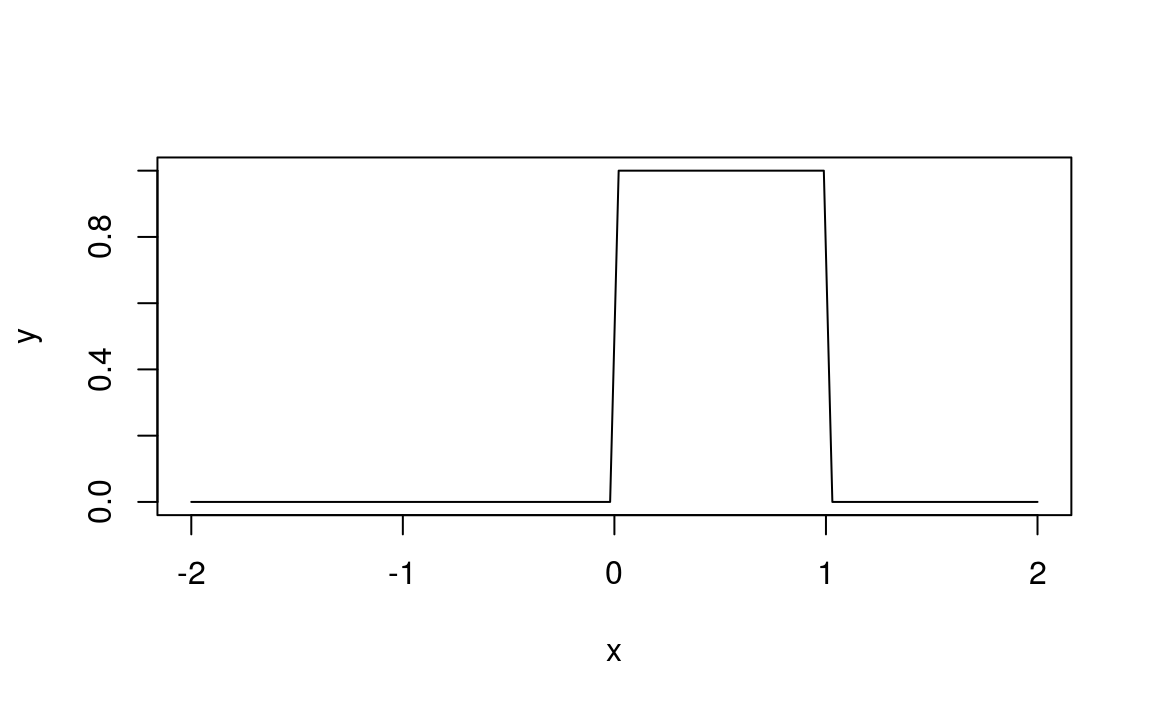
\includegraphics[width=0.7\linewidth]{Machine-Learning_files/figure-latex/unnamed-chunk-16-3} \end{center}

\begin{Shaded}
\begin{Highlighting}[]

\CommentTok{# Computing the 95% quantile for a U(0, 1)}
\KeywordTok{qunif}\NormalTok{(}\DataTypeTok{p =} \FloatTok{0.95}\NormalTok{, }\DataTypeTok{min =} \DecValTok{0}\NormalTok{, }\DataTypeTok{max =} \DecValTok{1}\NormalTok{)}
\CommentTok{#ans> [1] 0.95}
\end{Highlighting}
\end{Shaded}

\begin{rmdexercise}
Do the following:

\begin{itemize}
\tightlist
\item
  Compute the 90\%, 95\% and 99\% quantiles of a \(F\) distribution with
  \texttt{df1\ =\ 1} and \texttt{df2\ =\ 5}. (Answer:
  \texttt{c(4.060420,\ 6.607891,\ 16.258177)})
\item
  Sample 100 points from a Poisson with \texttt{lambda\ =\ 5}.
\item
  Plot the density of a \(t\) distribution with \texttt{df\ =\ 1} (use a
  sequence spanning from \texttt{-4} to \texttt{4}). Add lines of
  different colors with the densities for \texttt{df\ =\ 5},
  \texttt{df\ =\ 10}, \texttt{df\ =\ 50} and \texttt{df\ =\ 100}.
\end{itemize}
\end{rmdexercise}

\subsection{Working directory}\label{working-directory}

Your \emph{working directory} is the folder on your computer in which
you are currently working. When you ask R to open a certain file, it
will look in the working directory for this file, and when you tell R to
save a data file or figure, it will save it in the working directory.

To set your working directory within RStudio you can go to
\texttt{Tools\ /\ Set\ working\ directory}, or use the command
\texttt{setwd()}, we put the complete path of the directory between the
brackets, do not forget to put the path into quotation marks
\texttt{""}.

To know the actual working directory we use \texttt{getwd()}.

\subsection{Loading Data}\label{loading-data}

The \texttt{read.table()} function is one of the primary ways to import
a data set into \texttt{R}. The help file \texttt{?read.table()}
contains details about how to use this function. We can use the function
\texttt{write.table()} to export data.

Next we will show how to load the data set
\href{datasets/Auto.data}{\texttt{Auto.data}}.

\begin{Shaded}
\begin{Highlighting}[]
\NormalTok{Auto=}\KeywordTok{read.table}\NormalTok{(}\StringTok{"Auto.data"}\NormalTok{,}\DataTypeTok{header=}\NormalTok{T,}\DataTypeTok{na.strings =}\StringTok{"?"}\NormalTok{)}
\CommentTok{# For this file we needed to tell R that the first row is the}
\CommentTok{# names of the variables.}
\CommentTok{# na.strings tells R that any time it sees a particular character}
\CommentTok{# or set of characters (such as a question mark), it should be}
\CommentTok{# treated as a missing element of the data matrix. }
\end{Highlighting}
\end{Shaded}

\begin{rmdinsight}
\begin{itemize}
\tightlist
\item
  If the file is of csv format, we use \texttt{read.csv}.
\item
  Always try to look to the file before importing it to \texttt{R} (Open
  it in a text editor. See for example if the first row containes the
  variables names, if the columns are separated by \texttt{,} or
  \texttt{;} or ..
\item
  For text editors, I suggest
  \href{https://www.sublimetext.com/}{\texttt{Sublime\ Text}} or
  \href{https://atom.io/}{\texttt{Atom}}.
\end{itemize}
\end{rmdinsight}

\begin{Shaded}
\begin{Highlighting}[]
\KeywordTok{dim}\NormalTok{(Auto) }\CommentTok{# To see the dimensions of the data set}
\CommentTok{#ans> [1] 397   9}
\KeywordTok{nrow}\NormalTok{(Auto) }\CommentTok{# To see the number of rows}
\CommentTok{#ans> [1] 397}
\KeywordTok{ncol}\NormalTok{(Auto) }\CommentTok{# To see the number of columns}
\CommentTok{#ans> [1] 9}
\NormalTok{Auto[}\DecValTok{1}\NormalTok{:}\DecValTok{4}\NormalTok{,] }\CommentTok{# The first 4 rows of the data set}
\CommentTok{#ans>   mpg cylinders displacement horsepower weight acceleration year origin}
\CommentTok{#ans> 1  18         8          307        130   3504         12.0   70      1}
\CommentTok{#ans> 2  15         8          350        165   3693         11.5   70      1}
\CommentTok{#ans> 3  18         8          318        150   3436         11.0   70      1}
\CommentTok{#ans> 4  16         8          304        150   3433         12.0   70      1}
\CommentTok{#ans>                        name}
\CommentTok{#ans> 1 chevrolet chevelle malibu}
\CommentTok{#ans> 2         buick skylark 320}
\CommentTok{#ans> 3        plymouth satellite}
\CommentTok{#ans> 4             amc rebel sst}
\end{Highlighting}
\end{Shaded}

\begin{Shaded}
\begin{Highlighting}[]
\CommentTok{# Once the data are loaded correctly, we can use names()}
\CommentTok{# to check the variable names.}
\KeywordTok{names}\NormalTok{(Auto)}
\CommentTok{#ans> [1] "mpg"          "cylinders"    "displacement" "horsepower"  }
\CommentTok{#ans> [5] "weight"       "acceleration" "year"         "origin"      }
\CommentTok{#ans> [9] "name"}
\end{Highlighting}
\end{Shaded}

\begin{rmdinsight}
Take a look at this
\href{https://cran.r-project.org/doc/contrib/Torfs+Brauer-Short-R-Intro.pdf}{(very)
short introduction to R}. It can be useful.
\end{rmdinsight}

\section{Regression}\label{regression}

\subsection{\texorpdfstring{The \texttt{lm}
function}{The lm function}}\label{the-lm-function}

We are going to employ the \texttt{EU} dataset. The \texttt{EU} dataset
contains 28 rows with the member states of the European Union (Country),
the number of seats assigned under different years (Seats2011,
Seats2014), the Cambridge Compromise apportionment (CamCom2011), and the
countries population (Population2010,Population2013).

\begin{Shaded}
\begin{Highlighting}[]
\CommentTok{# Load the dataset, when we load an .RData using load()}
\CommentTok{# function we do not attribute it to a name like we did}
\CommentTok{# when we used read.table() or when we use read.csv()}

\KeywordTok{load}\NormalTok{(}\StringTok{"EU.RData"}\NormalTok{)}
\end{Highlighting}
\end{Shaded}

\begin{rmdinsight}
There is two ways to tell \texttt{R} where is the file you want to
load/use/import or where to save a file when you write/export/save :

\begin{enumerate}
\def\labelenumi{\arabic{enumi}.}
\tightlist
\item
  write the complete path of the files.
\item
  set a working directory and put the files in it.
\end{enumerate}
\end{rmdinsight}

\begin{Shaded}
\begin{Highlighting}[]
\CommentTok{# lm (for linear model) has the syntax: }
\CommentTok{# lm(formula = response ~ predictor, data = data)}
\CommentTok{# The response is the y in the model. The predictor is x.}
\CommentTok{# For example (after loading the EU dataset)}
\NormalTok{mod <-}\StringTok{ }\KeywordTok{lm}\NormalTok{(}\DataTypeTok{formula =} \NormalTok{Seats2011 ~}\StringTok{ }\NormalTok{Population2010, }\DataTypeTok{data =} \NormalTok{EU)}

\CommentTok{# We have saved the linear model into mod, which now contains all the output of lm}
\CommentTok{# You can see it by typing}
\NormalTok{mod}
\CommentTok{#ans> }
\CommentTok{#ans> Call:}
\CommentTok{#ans> lm(formula = Seats2011 ~ Population2010, data = EU)}
\CommentTok{#ans> }
\CommentTok{#ans> Coefficients:}
\CommentTok{#ans>    (Intercept)  Population2010  }
\CommentTok{#ans>       7.91e+00        1.08e-06}

\CommentTok{# mod is indeed a list of objects whose names are}
\KeywordTok{names}\NormalTok{(mod)}
\CommentTok{#ans>  [1] "coefficients"  "residuals"     "effects"       "rank"         }
\CommentTok{#ans>  [5] "fitted.values" "assign"        "qr"            "df.residual"  }
\CommentTok{#ans>  [9] "na.action"     "xlevels"       "call"          "terms"        }
\CommentTok{#ans> [13] "model"}

\CommentTok{# We can access these elements by $}
\CommentTok{# For example}
\NormalTok{mod$coefficients}
\CommentTok{#ans>    (Intercept) Population2010 }
\CommentTok{#ans>       7.91e+00       1.08e-06}

\CommentTok{# The residuals}
\NormalTok{mod$residuals}
\CommentTok{#ans>        Germany         France United Kingdom          Italy          Spain }
\CommentTok{#ans>         2.8675        -3.7031        -1.7847         0.0139        -3.5084 }
\CommentTok{#ans>         Poland        Romania    Netherlands         Greece        Belgium }
\CommentTok{#ans>         1.9272         1.9434         0.2142         1.8977         2.3994 }
\CommentTok{#ans>       Portugal Czech Republic        Hungary         Sweden        Austria }
\CommentTok{#ans>         2.6175         2.7587         3.2898         2.0163         2.0575 }
\CommentTok{#ans>       Bulgaria        Denmark       Slovakia        Finland        Ireland }
\CommentTok{#ans>         1.9328        -0.8790        -0.7606        -0.6813        -0.7284 }
\CommentTok{#ans>      Lithuania         Latvia       Slovenia        Estonia         Cyprus }
\CommentTok{#ans>         0.4998        -1.3347        -2.1175        -3.3552        -2.7761 }
\CommentTok{#ans>     Luxembourg          Malta }
\CommentTok{#ans>        -2.4514        -2.3553}

\CommentTok{# The fitted values}
\NormalTok{mod$fitted.values}
\CommentTok{#ans>        Germany         France United Kingdom          Italy          Spain }
\CommentTok{#ans>          96.13          77.70          74.78          72.99          57.51 }
\CommentTok{#ans>         Poland        Romania    Netherlands         Greece        Belgium }
\CommentTok{#ans>          49.07          31.06          25.79          20.10          19.60 }
\CommentTok{#ans>       Portugal Czech Republic        Hungary         Sweden        Austria }
\CommentTok{#ans>          19.38          19.24          18.71          17.98          16.94 }
\CommentTok{#ans>       Bulgaria        Denmark       Slovakia        Finland        Ireland }
\CommentTok{#ans>          16.07          13.88          13.76          13.68          12.73 }
\CommentTok{#ans>      Lithuania         Latvia       Slovenia        Estonia         Cyprus }
\CommentTok{#ans>          11.50          10.33          10.12           9.36           8.78 }
\CommentTok{#ans>     Luxembourg          Malta }
\CommentTok{#ans>           8.45           8.36}

\CommentTok{# Summary of the model}
\NormalTok{sumMod <-}\StringTok{ }\KeywordTok{summary}\NormalTok{(mod)}
\NormalTok{sumMod}
\CommentTok{#ans> }
\CommentTok{#ans> Call:}
\CommentTok{#ans> lm(formula = Seats2011 ~ Population2010, data = EU)}
\CommentTok{#ans> }
\CommentTok{#ans> Residuals:}
\CommentTok{#ans>    Min     1Q Median     3Q    Max }
\CommentTok{#ans> -3.703 -1.951  0.014  1.980  3.290 }
\CommentTok{#ans> }
\CommentTok{#ans> Coefficients:}
\CommentTok{#ans>                Estimate Std. Error t value Pr(>|t|)    }
\CommentTok{#ans> (Intercept)    7.91e+00   5.66e-01    14.0  2.6e-13 ***}
\CommentTok{#ans> Population2010 1.08e-06   1.92e-08    56.3  < 2e-16 ***}
\CommentTok{#ans> ---}
\CommentTok{#ans> Signif. codes:  0 '***' 0.001 '**' 0.01 '*' 0.05 '.' 0.1 ' ' 1}
\CommentTok{#ans> }
\CommentTok{#ans> Residual standard error: 2.29 on 25 degrees of freedom}
\CommentTok{#ans>   (1 observation deleted due to missingness)}
\CommentTok{#ans> Multiple R-squared:  0.992,   Adjusted R-squared:  0.992 }
\CommentTok{#ans> F-statistic: 3.17e+03 on 1 and 25 DF,  p-value: <2e-16}
\end{Highlighting}
\end{Shaded}

The following table contains a handy cheat sheet of equivalences between
\texttt{R} code and some of the statistical concepts associated to
linear regression.

\begin{longtable}[]{@{}ll@{}}
\toprule
\begin{minipage}[b]{0.49\columnwidth}\raggedright\strut
\texttt{R}\strut
\end{minipage} & \begin{minipage}[b]{0.45\columnwidth}\raggedright\strut
Statistical concept\strut
\end{minipage}\tabularnewline
\midrule
\endhead
\begin{minipage}[t]{0.49\columnwidth}\raggedright\strut
\texttt{x}\strut
\end{minipage} & \begin{minipage}[t]{0.45\columnwidth}\raggedright\strut
Predictor \(X_1,\ldots,X_n\)\strut
\end{minipage}\tabularnewline
\begin{minipage}[t]{0.49\columnwidth}\raggedright\strut
\texttt{y}\strut
\end{minipage} & \begin{minipage}[t]{0.45\columnwidth}\raggedright\strut
Response \(Y_1,\ldots,Y_n\)\strut
\end{minipage}\tabularnewline
\begin{minipage}[t]{0.49\columnwidth}\raggedright\strut
\texttt{data\ \textless{}-\ data.frame(x\ =\ x,\ y\ =\ y)}\strut
\end{minipage} & \begin{minipage}[t]{0.45\columnwidth}\raggedright\strut
Sample \((X_1,Y_1),\ldots,(X_n,Y_n)\)\strut
\end{minipage}\tabularnewline
\begin{minipage}[t]{0.49\columnwidth}\raggedright\strut
\texttt{model\ \textless{}-\ lm(y\ \textasciitilde{}\ x,\ data\ =\ data)}\strut
\end{minipage} & \begin{minipage}[t]{0.45\columnwidth}\raggedright\strut
Fitted linear model\strut
\end{minipage}\tabularnewline
\begin{minipage}[t]{0.49\columnwidth}\raggedright\strut
\texttt{model\$coefficients}\strut
\end{minipage} & \begin{minipage}[t]{0.45\columnwidth}\raggedright\strut
Fitted coefficients \(\hat\beta_0,\hat\beta_1\)\strut
\end{minipage}\tabularnewline
\begin{minipage}[t]{0.49\columnwidth}\raggedright\strut
\texttt{model\$residuals}\strut
\end{minipage} & \begin{minipage}[t]{0.45\columnwidth}\raggedright\strut
Fitted residuals \(\hat\varepsilon_1,\ldots,\hat\varepsilon_n\)\strut
\end{minipage}\tabularnewline
\begin{minipage}[t]{0.49\columnwidth}\raggedright\strut
\texttt{model\$fitted.values}\strut
\end{minipage} & \begin{minipage}[t]{0.45\columnwidth}\raggedright\strut
Fitted values \(\hat Y_1,\ldots,\hat Y_n\)\strut
\end{minipage}\tabularnewline
\begin{minipage}[t]{0.49\columnwidth}\raggedright\strut
\texttt{model\$df.residual}\strut
\end{minipage} & \begin{minipage}[t]{0.45\columnwidth}\raggedright\strut
Degrees of freedom \(n-2\)\strut
\end{minipage}\tabularnewline
\begin{minipage}[t]{0.49\columnwidth}\raggedright\strut
\texttt{summaryModel\ \textless{}-\ summary(model)}\strut
\end{minipage} & \begin{minipage}[t]{0.45\columnwidth}\raggedright\strut
Summary of the fitted linear model\strut
\end{minipage}\tabularnewline
\begin{minipage}[t]{0.49\columnwidth}\raggedright\strut
\texttt{summaryModel\$sigma}\strut
\end{minipage} & \begin{minipage}[t]{0.45\columnwidth}\raggedright\strut
Fitted residual standard deviation \(\hat\sigma\)\strut
\end{minipage}\tabularnewline
\begin{minipage}[t]{0.49\columnwidth}\raggedright\strut
\texttt{summaryModel\$r.squared}\strut
\end{minipage} & \begin{minipage}[t]{0.45\columnwidth}\raggedright\strut
Coefficient of determination \(R^2\)\strut
\end{minipage}\tabularnewline
\begin{minipage}[t]{0.49\columnwidth}\raggedright\strut
\texttt{summaryModel\$fstatistic}\strut
\end{minipage} & \begin{minipage}[t]{0.45\columnwidth}\raggedright\strut
\(F\)-test\strut
\end{minipage}\tabularnewline
\begin{minipage}[t]{0.49\columnwidth}\raggedright\strut
\texttt{anova(model)}\strut
\end{minipage} & \begin{minipage}[t]{0.45\columnwidth}\raggedright\strut
ANOVA table\strut
\end{minipage}\tabularnewline
\bottomrule
\end{longtable}

\begin{rmdexercise}
Do the following:

\begin{itemize}
\tightlist
\item
  Download The `EU' dataset from \href{datasets/EU.RData}{here} as an
  \texttt{.RData} file and load it using the function \texttt{load}.
\item
  Compute the regression of \texttt{CamCom2011} into
  \texttt{Population2010}. Save that model as the variable
  \texttt{myModel}.
\item
  Access the objects \texttt{residuals} and \texttt{coefficients} of
  \texttt{myModel}.
\item
  Compute the summary of \texttt{myModel} and store it as the variable
  \texttt{summaryMyModel}.
\item
  Access the object \texttt{sigma} of \texttt{myModel}.
\end{itemize}
\end{rmdexercise}

\subsection{Predicting House Value: Boston
dataset}\label{predicting-house-value-boston-dataset}

We are going to use a dataset called Boston which is part of the
\texttt{MASS} package. It recordes the median value of houses for 506
neighborhoods around Boston. Our task is to predict the median house
value (\texttt{medv}) using only one predictor (\texttt{lstat}: percent
of households with low socioeconomic status).

\begin{Shaded}
\begin{Highlighting}[]
\CommentTok{# First, install the MASS package using the command: install.packages("MASS")}

\CommentTok{# load MASS package}
\KeywordTok{library}\NormalTok{(MASS)}

\CommentTok{# Check the dimensions of the Boston dataset}
\KeywordTok{dim}\NormalTok{(Boston)}
\CommentTok{#ans> [1] 506  14}
\end{Highlighting}
\end{Shaded}

\textbf{STEP 1: Split the dataset}

\begin{Shaded}
\begin{Highlighting}[]
\CommentTok{# Split the data by using the first 400 observations as the training}
\CommentTok{# data and the remaining as the testing data}
\NormalTok{train =}\StringTok{ }\DecValTok{1}\NormalTok{:}\DecValTok{400}
\NormalTok{test =}\StringTok{ }\NormalTok{-train}

\CommentTok{# Speficy that we are going to use only two variables (lstat and medv)}
\NormalTok{variables =}\StringTok{ }\KeywordTok{which}\NormalTok{(}\KeywordTok{names}\NormalTok{(Boston) ==}\KeywordTok{c}\NormalTok{(}\StringTok{"lstat"}\NormalTok{, }\StringTok{"medv"}\NormalTok{))}
\NormalTok{training_data =}\StringTok{ }\NormalTok{Boston[train, variables]}
\NormalTok{testing_data =}\StringTok{ }\NormalTok{Boston[test, variables]}

\CommentTok{# Check the dimensions of the new dataset}
\KeywordTok{dim}\NormalTok{(training_data)}
\CommentTok{#ans> [1] 400   2}
\end{Highlighting}
\end{Shaded}

\textbf{STEP 2: Check for Linearity}

In order to perfom linear regression in \texttt{R}, we will use the
function \texttt{lm()}to fit a simple linear regression with
\texttt{medv} as the response (dependent variable) and \texttt{lstat} as
the predictor or independent variable, and then save it in
\texttt{model}.

But before we run our model, let's visually check if the relationship
between x and y is linear.

\begin{Shaded}
\begin{Highlighting}[]
\CommentTok{# Scatterplot of lstat vs. medv}
\KeywordTok{plot}\NormalTok{(training_data$lstat, training_data$medv)}
\end{Highlighting}
\end{Shaded}

\begin{center}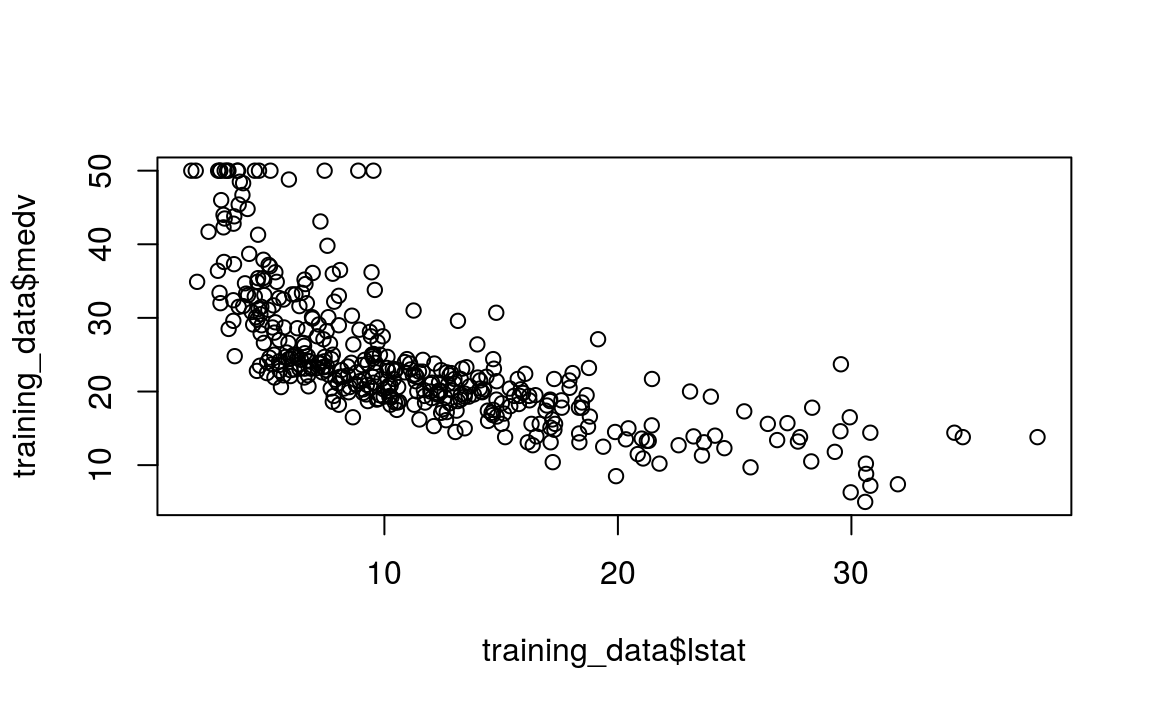
\includegraphics[width=0.7\linewidth]{Machine-Learning_files/figure-latex/unnamed-chunk-31-1} \end{center}

According to the plot, we see that the relationship is not linear. Let's
try a transformation of our explanatory variable \texttt{lstat}.

\begin{Shaded}
\begin{Highlighting}[]
\CommentTok{# Scatterplot of log(lstat) vs. medv}
\KeywordTok{plot}\NormalTok{(}\KeywordTok{log}\NormalTok{(training_data$lstat), training_data$medv)}
\end{Highlighting}
\end{Shaded}

\begin{center}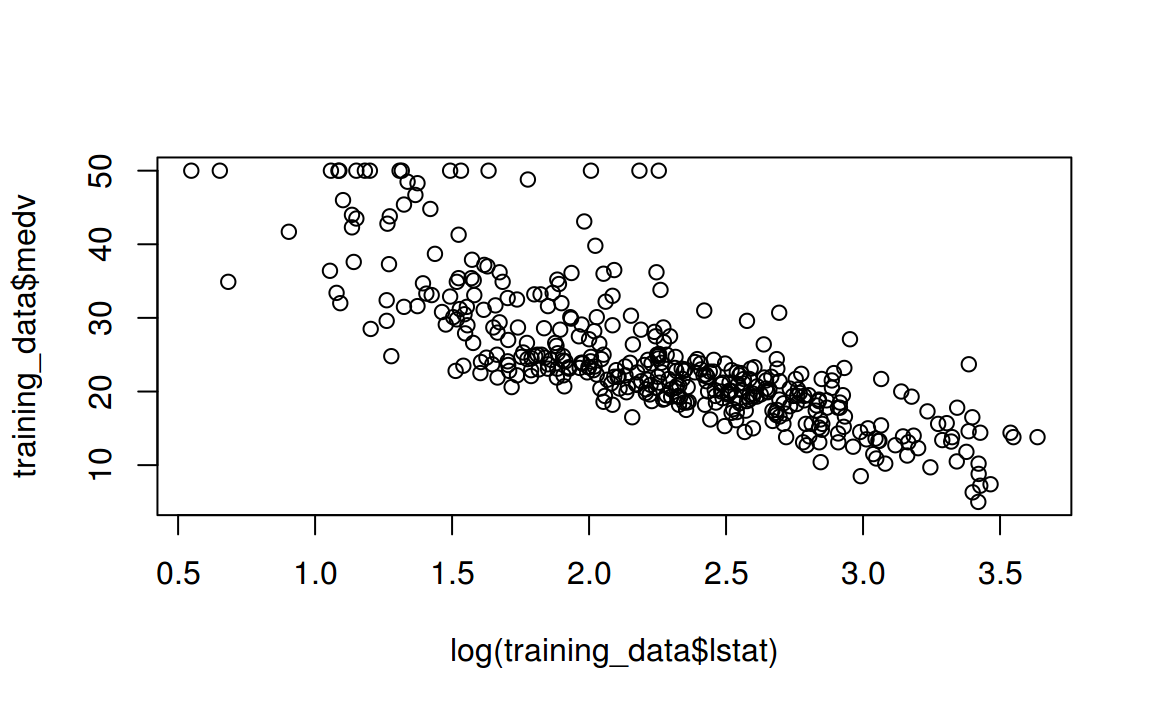
\includegraphics[width=0.7\linewidth]{Machine-Learning_files/figure-latex/unnamed-chunk-32-1} \end{center}

Look at the plot, it is more linear, so we can proceed and perform
\texttt{lm()}:

\textbf{STEP 3: Run the linear regression model}

\begin{Shaded}
\begin{Highlighting}[]
\NormalTok{model =}\StringTok{ }\KeywordTok{lm}\NormalTok{(medv ~}\StringTok{ }\KeywordTok{log}\NormalTok{(lstat), }\DataTypeTok{data =} \NormalTok{training_data)}
\NormalTok{model}
\CommentTok{#ans> }
\CommentTok{#ans> Call:}
\CommentTok{#ans> lm(formula = medv ~ log(lstat), data = training_data)}
\CommentTok{#ans> }
\CommentTok{#ans> Coefficients:}
\CommentTok{#ans> (Intercept)   log(lstat)  }
\CommentTok{#ans>        51.8        -12.2}
\end{Highlighting}
\end{Shaded}

Notice that basic information when we print \texttt{model}. This only
give us the slope \((-12.2)\) and the intercept \((51.8)\) of the linear
model. Note that here we are looking at \texttt{log(lstat)} and not
\texttt{lstat} anymore. So for every one unit increase in
\texttt{lstat}, the median value of the house will decrease by
\(e^{12.2}\). For more detailed information, we can use the
\texttt{summary()} function:

\begin{Shaded}
\begin{Highlighting}[]
\KeywordTok{summary}\NormalTok{(model)}
\CommentTok{#ans> }
\CommentTok{#ans> Call:}
\CommentTok{#ans> lm(formula = medv ~ log(lstat), data = training_data)}
\CommentTok{#ans> }
\CommentTok{#ans> Residuals:}
\CommentTok{#ans>     Min      1Q  Median      3Q     Max }
\CommentTok{#ans> -11.385  -3.908  -0.779   2.245  25.728 }
\CommentTok{#ans> }
\CommentTok{#ans> Coefficients:}
\CommentTok{#ans>             Estimate Std. Error t value Pr(>|t|)    }
\CommentTok{#ans> (Intercept)   51.783      1.097    47.2   <2e-16 ***}
\CommentTok{#ans> log(lstat)   -12.203      0.472   -25.9   <2e-16 ***}
\CommentTok{#ans> ---}
\CommentTok{#ans> Signif. codes:  0 '***' 0.001 '**' 0.01 '*' 0.05 '.' 0.1 ' ' 1}
\CommentTok{#ans> }
\CommentTok{#ans> Residual standard error: 5.6 on 398 degrees of freedom}
\CommentTok{#ans> Multiple R-squared:  0.627,   Adjusted R-squared:  0.626 }
\CommentTok{#ans> F-statistic:  669 on 1 and 398 DF,  p-value: <2e-16}
\end{Highlighting}
\end{Shaded}

Now, we have access to p-values and standard errors for the
coefficients, as well as the \(R^2\).

\begin{itemize}
\tightlist
\item
  The output states that the slope is statistically significant and
  different from \(0\) and with a t-value= \(-25.9\) (p-value
  \(< 0.05\)), which means that there is a significant relationship
  between the percentage of households with low socioeconomic income and
  the median house value.
\item
  This relationship is negative. That is as the percantage of household
  with low socioeconomic income increases, the median house value
  decreases.
\item
  Looking at \(R^2\), we can deduce that \(62.7\%\) of the model
  variation is being explained by the predictor \texttt{log(lstat)}.
  This is probably low, but indeed it would increase if we had more
  independent (explanatory) variables. We can use the \texttt{names()}
  function to see what other pieces of information are stored in our
  linear model (\texttt{model}).
\end{itemize}

\begin{Shaded}
\begin{Highlighting}[]
\KeywordTok{names}\NormalTok{(model)}
\CommentTok{#ans>  [1] "coefficients"  "residuals"     "effects"       "rank"         }
\CommentTok{#ans>  [5] "fitted.values" "assign"        "qr"            "df.residual"  }
\CommentTok{#ans>  [9] "xlevels"       "call"          "terms"         "model"}
\end{Highlighting}
\end{Shaded}

\begin{Shaded}
\begin{Highlighting}[]
\NormalTok{model$coefficients}
\CommentTok{#ans> (Intercept)  log(lstat) }
\CommentTok{#ans>        51.8       -12.2}
\end{Highlighting}
\end{Shaded}

To obtain the confidence intervel for the linear model (\texttt{model}),
we can use the \texttt{confint()} function:

\begin{Shaded}
\begin{Highlighting}[]
\KeywordTok{confint}\NormalTok{(model, }\DataTypeTok{level =} \FloatTok{0.95}\NormalTok{)}
\CommentTok{#ans>             2.5 % 97.5 %}
\CommentTok{#ans> (Intercept)  49.6   53.9}
\CommentTok{#ans> log(lstat)  -13.1  -11.3}
\end{Highlighting}
\end{Shaded}

So, a \(95\%\) confidence interval for the slope of \texttt{log(lstat)}
is \((-13.13, -11.28)\). Notice that this confidence interval gives us
the same result as the hypothesis test performed earlier, by stating
that we are \(95\%\) confident that the slope of \texttt{lstat} is not
zero (in fact it is less than zero, which means that the relationship is
negative.)

\textbf{STEP 4: Plot the regression model}

Now, let's plot our regression line on top of our data.

\begin{Shaded}
\begin{Highlighting}[]
\CommentTok{# Scatterplot of lstat vs. medv}
\KeywordTok{plot}\NormalTok{(}\KeywordTok{log}\NormalTok{(training_data$lstat), training_data$medv)}

\CommentTok{# Add the regression line to the existing scatterplot}
\KeywordTok{abline}\NormalTok{(model)}
\end{Highlighting}
\end{Shaded}

\begin{center}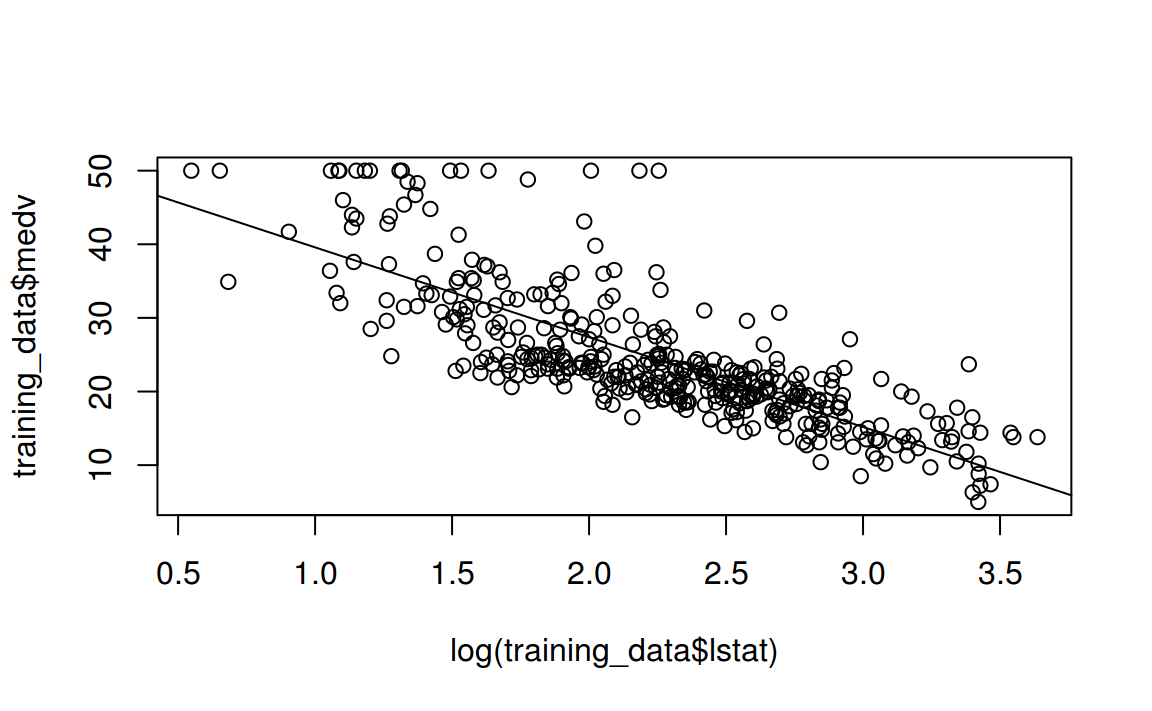
\includegraphics[width=0.7\linewidth]{Machine-Learning_files/figure-latex/unnamed-chunk-38-1} \end{center}

Let's play with the look of the plot, and makes it perttier!

\begin{Shaded}
\begin{Highlighting}[]
\CommentTok{# Scatterplot of lstat vs. medv}
\KeywordTok{plot}\NormalTok{(}\KeywordTok{log}\NormalTok{(training_data$lstat), training_data$medv,}
\DataTypeTok{xlab =} \StringTok{"Log Transform of % of Houshold with Low Socioeconomic Income"}\NormalTok{,}
\DataTypeTok{ylab =} \StringTok{"Median House Value"}\NormalTok{,}
\DataTypeTok{col =} \StringTok{"red"}\NormalTok{,}
\DataTypeTok{pch =} \DecValTok{20}\NormalTok{)}

\CommentTok{# Make the line color blue, and the line's width =3 (play with the width!)}
\KeywordTok{abline}\NormalTok{(model, }\DataTypeTok{col =} \StringTok{"blue"}\NormalTok{, }\DataTypeTok{lwd =}\DecValTok{3}\NormalTok{)}
\end{Highlighting}
\end{Shaded}

\begin{center}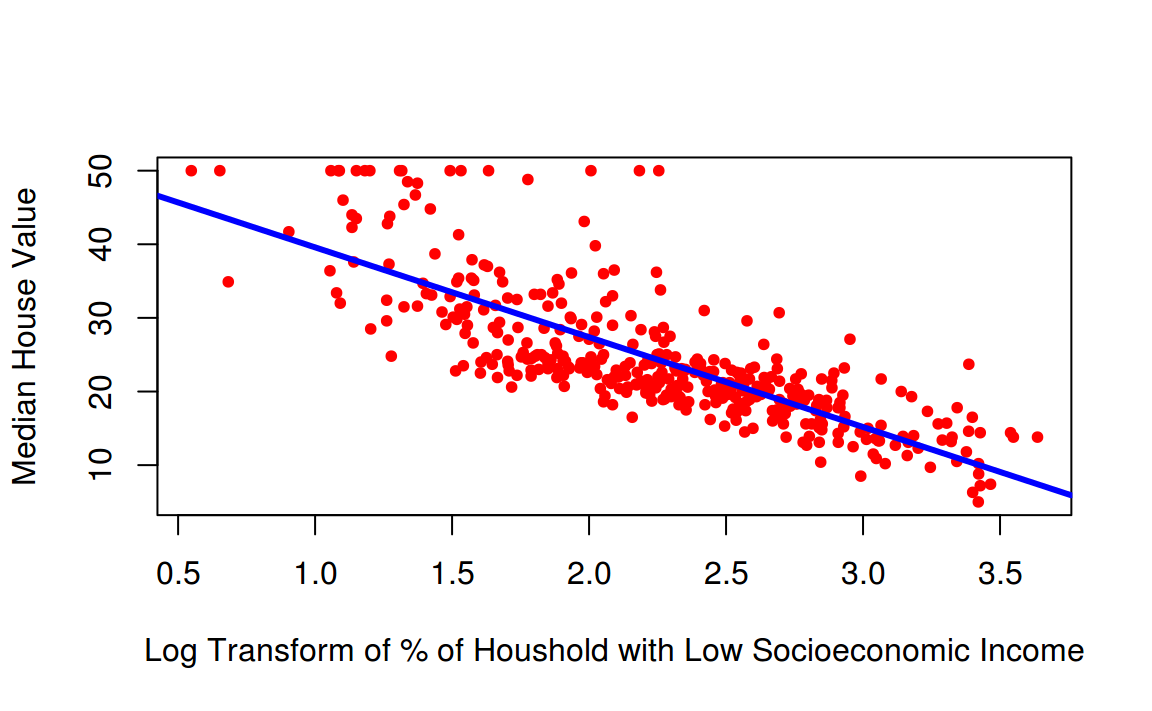
\includegraphics[width=0.7\linewidth]{Machine-Learning_files/figure-latex/unnamed-chunk-39-1} \end{center}

\textbf{STEP 5: Assess the model}

Final thing we will do is to predict using our fitted model. We can use
the \texttt{predict()} function for this purpose:

\begin{Shaded}
\begin{Highlighting}[]
\CommentTok{# Predict what is the median value of the house with lstat= 5%}
\KeywordTok{predict}\NormalTok{(model, }\KeywordTok{data.frame}\NormalTok{(}\DataTypeTok{lstat =} \KeywordTok{c}\NormalTok{(}\DecValTok{5}\NormalTok{)))}
\CommentTok{#ans>    1 }
\CommentTok{#ans> 32.1}
\end{Highlighting}
\end{Shaded}

\begin{Shaded}
\begin{Highlighting}[]
\CommentTok{# Predict what is the median values of houses with lstat= 5%, 10%, and 15%}
\KeywordTok{predict}\NormalTok{(model, }\KeywordTok{data.frame}\NormalTok{(}\DataTypeTok{lstat =} \KeywordTok{c}\NormalTok{(}\DecValTok{5}\NormalTok{,}\DecValTok{10}\NormalTok{,}\DecValTok{15}\NormalTok{), }\DataTypeTok{interval =} \StringTok{"prediction"}\NormalTok{))}
\CommentTok{#ans>    1    2    3 }
\CommentTok{#ans> 32.1 23.7 18.7}
\end{Highlighting}
\end{Shaded}

Now let's assess our model, by computing th mean squared error (MSE). To
assess the model we created, then we will be using the test data!

\begin{Shaded}
\begin{Highlighting}[]
\CommentTok{# Save the testing median values for houses (testing y) in y}
\NormalTok{y =}\StringTok{ }\NormalTok{testing_data$medv}

\CommentTok{# Compute the predicted value for this y (y hat)}
\NormalTok{y_hat =}\StringTok{ }\KeywordTok{predict}\NormalTok{(model, }\KeywordTok{data.frame}\NormalTok{(}\DataTypeTok{lstat =} \NormalTok{testing_data$lstat))}

\CommentTok{# Now we have both y and y_hat for our testing data. }
\CommentTok{# let's find the mean square error}
\NormalTok{error =}\StringTok{ }\NormalTok{y-y_hat}
\NormalTok{error_squared =}\StringTok{ }\NormalTok{error^}\DecValTok{2}
\NormalTok{MSE =}\StringTok{ }\KeywordTok{mean}\NormalTok{(error_squared)}
\NormalTok{MSE}
\CommentTok{#ans> [1] 17.7}
\end{Highlighting}
\end{Shaded}

◼

\chapter{Multiple Linear Regression}\label{multiple-linear-regression}

Simple linear regression is a useful approach for predicting a response
on the basis of a single predictor variable. However, in practice we
often have more than one predictor. In the previous chapter, we took for
example the prediction of housing prices considering we had the size of
each house. We had a single feature \(X\), the size of the house. But
now imagine if we had not only the size of the house as a feature but we
also knew the number of bedrooms, the number of flours and the age of
the house in years. It seems like this would give us a lot more
information with which to predict the price.

\section{The Model}\label{the-model}

In general, suppose that we have \(p\) distinct predictors. Then the
multiple linear regression model takes the form

\[ Y = \beta_0 + \beta_1 X_1 + \beta_2 X_2 + \dots + \beta_p X_p + \epsilon \]

where \(X_j\) represents the \(j\)th predictor and \(\beta_j\)
quantifies the association between that variable and the response. We
interpret \(\beta_j\) as the average effect on \(Y\) of a one unit
increase in \(X_j\), \emph{holding all other predictors fixed}.

In matrix terms, supposing we have \(n\) observations and \(p\)
variables, we need to define the following matrices:

\begin{equation}
 \textbf{Y}_{n \times 1} = \begin{pmatrix}
    Y_{1} \\
    Y_{2} \\
    \vdots \\
    Y_{n}
\end{pmatrix}   \,\,\,\,\,\,\,\,\,\,\,\,  \textbf{X}_{n \times (p+1)}  = \begin{pmatrix}
    1      & X_{11} & X_{12} & \dots  & X_{1p} \\
    1      & X_{21} & X_{22} & \dots  & X_{2p} \\
    \vdots & \vdots & \vdots & \ddots & \vdots \\
    1      & X_{n1} & X_{n2} & \dots  & X_{np}
\end{pmatrix}
\end{equation}

\begin{equation}
 {\mathbb{\beta}}_{(p+1) \times 1} = \begin{pmatrix}
    \beta_{0} \\
    \beta_{1} \\
    \vdots \\
    \beta_{p}
    \end{pmatrix}   \,\,\,\,\,\,\,\,\,\,\,\,  {\epsilon}_{n \times 1} = \begin{pmatrix}
        \epsilon_{1} \\
        \epsilon_{2} \\
        \vdots \\
        \epsilon_{n}
    \end{pmatrix}
\end{equation}

In matrix terms, the general linear regression model is

\[ \textbf{Y}_{n \times 1} = \textbf{X}_{n \times (p+1)} {\mathbb{\beta}}_{(p+1) \times 1} + {\epsilon}_{n \times 1} \]

where,

\begin{itemize}
\tightlist
\item
  \(\textbf{Y}\) is a vector of responses.
\item
  \(\mathbb{\beta}\) is a vector of parameters.
\item
  \(\textbf{X}\) is a matrix of constants.
\item
  \(\epsilon\) is a vector of independent \emph{normal} (Gaussian)
  random variables.
\end{itemize}

\section{Estimating the Regression
Coefficients}\label{estimating-the-regression-coefficients}

As was the case in the simple linear regression setting, the regression
coefficients \(\beta_{0}, \beta_{1}, \ldots, \beta_{p}\) are unknown,
and must be estimated. Given estimates
\(\hat{\beta_{0}}, \hat{\beta_{1}}, \ldots, \hat{\beta_{p}}\), we can
make predictions using the formula

\[ \hat{y} = \hat{\beta_{0}} + \hat{\beta_{1}} x_1 + \hat{\beta_{2}} x_2 + \ldots, \hat{\beta_{p}} x_p \]

We choose \(\beta_{0}, \beta_{1}, \ldots, \beta_{p}\) to minimize the
sum of squared residuals

\[ \begin{aligned}
RSS &= \sum_{i=1}^{n} (y_i - \hat{y}_i)^2 \\
    &= \sum_{i=1}^{n} (y_1 - \hat{\beta_0} - \hat{\beta_1} \hat{x}_{i1}  - \hat{\beta_2} \hat{x}_{i2} - \ldots  -  \hat{\beta_p} \hat{x}_{ip})^2 \\
\end{aligned}
\]

The values \(\hat{\beta_{0}}, \hat{\beta_{1}}, \ldots, \hat{\beta_{p}}\)
that minimize the RSS are the multiple least squares regression
coefficient estimates, they are calculated using this formula (in matrix
terms):

\[ \hat{\beta} = (\textbf{X}^T \textbf{X})^{-1}\textbf{X}^T \textbf{Y} \]

Note 1:

\begin{rmdinsight}
It is a remarkable property of matrix algebra that the results for the
general linear regression model in matrix notation appear exactly as
those for the simple linear regression model. Only the degrees of
freedom and other constants related to the number of \(X\) variables and
the dimensions of some matrices are different.
\end{rmdinsight}

Note 2:

\begin{rmdinsight}
If \(\textbf{X}^T \textbf{X}\) is noninvertible, the common causes might
be having:

\begin{itemize}
\tightlist
\item
  Redundant features, where two features are very closely related
  (i.e.~they are linearly dependent)
\item
  Too many features (e.g. \(p \geq n\)). In this case, we delete some
  features or we use ``regularization'' (to be, maybe, explained in a
  later lesson).
\end{itemize}
\end{rmdinsight}

\section{Some important questions}\label{some-important-questions}

When we perform multiple linear regression, we usually are interested in
answering a few important questions.

\begin{enumerate}
\def\labelenumi{\arabic{enumi}.}
\tightlist
\item
  Is at least one of the predictors \(X_1 ,X_2 ,\ldots,X_p\) useful in
  predicting the response?
\item
  Do all the predictors help to explain \(Y\), or is only a subset of
  the predictors useful?
\item
  How well does the model fit the data?
\item
  Given a set of predictor values, what response value should we
  predict, and how accurate is our prediction?
\end{enumerate}

\textbf{\emph{Relationship Between the Response and Predictors?}}

\textbf{\(F\)-Statistic}

Recall that in the simple linear regression setting, in order to
determine whether there is a relationship between the response and the
predictor we can simply check whether \(\beta_1 = 0\). In the multiple
regression setting with \(p\) predictors, we need to ask whether all of
the regression coefficients are zero, i.e.~whether
\(\beta_1 = \beta_2 = \ldots = \beta_p = 0\). As in the simple linear
regression setting, we use a hypothesis test to answer this question. We
test the null hypothesis,

\[ H_0 : \beta_1 = \beta_2 = \ldots = \beta_p = 0 \]

versus the alternative hypothesis

\[ H_1 : \text{at least one} \, \beta_j \, \text{is non-zero} \]

This hypothesis test is performed by computing the \(F\)-statistic
(\emph{Fisher}):

\[ F = \frac{ (\text{TSS} - \text{RSS})/p}{\text{RSS}/(n-p-1)} \sim F_{p,n-p-1} \]

where, as with simple linear regression,
\(\text{TSS} = \sum (y_i - \bar{y})^2\) and
\(\text{RSS} = \sum (y_i - \hat{y}_i)^2\).

When the \(F\)-statistic value is close to 1, then \(H_0\) is true,
which means there is no relationship between the response and
predictors. On the other hand, if \(H_1\) is true, so we expect \(F\) to
be greater than 1.

So the question we ask here: \emph{Is the whole regression explaining
anything at all?} The answer comes from the \(F\)-test in the ANOVA
(ANalysis Of VAriance) table. This is what we get in an ANOVA table:

\begin{longtable}[]{@{}llllll@{}}
\toprule
Source & df & SS & MS & \(F\) & p-value\tabularnewline
\midrule
\endhead
Factor (Explained) & \(p-1\) & SST & SST/\((k-1)\) & MST/MSE &
p-value\tabularnewline
Error (Unexplained) & \(n-p\) & SSE & SSE/\((n-k)\) & &\tabularnewline
Total & \(n-1\) & SS & & &\tabularnewline
\bottomrule
\end{longtable}

The ANOVA table has many pieces of information. What we care about is
the \(F\) Ratio and the corresponding p-value. We compare the \(F\)
Ratio with \(F_{(p-1,n-p)}\) and a corresponding \(\alpha\) value
(error).

\textbf{p-values}

The p-values provide information about whether each individual predictor
is related to the response, after adjusting for the other predictors.
Let's look at the following table we obtain in general using a
statistical software for example

\begin{longtable}[]{@{}lllll@{}}
\toprule
& Coefficient & Std. error & \(t\)-statistic & p-value\tabularnewline
\midrule
\endhead
Constant & 2.939 & 0.3119 & 9.42 & \textless{}0.0001\tabularnewline
\(X_1\) & 0.046 & 0.0014 & 32.81 & \textless{}0.0001\tabularnewline
\(X_2\) & 0.189 & 0.0086 & 21.89 & \textless{}0.0001\tabularnewline
\(X_3\) & -0.001 & 0.0059 & -0.18 & 0.8599\tabularnewline
\bottomrule
\end{longtable}

In this tablewe the following model

\[ Y = 2.939 + 0.046 X_1 + 0.189 X_2 - 0.001 X_3 \]

Note that for each individual predictor a \(t\)-statistic and a p-value
were reported. These p-values indicate that \(X_1\) and \(X_2\) are
related to \(Y\), but that there is no evidence that \(X_3\) is
associated with \(Y\), in the presence of these two.

\textbf{\emph{Deciding on Important Variables}}

The most direct approach is called \emph{all subsets} or \emph{best
subsets} regression: we compute the least squares fit for all possible
subsets and then choose between them based on some criterion that
balances training error with model size.

However we often can't examine all possible models, since they are
\(2^p\) of them; for example when \(p = 40\) there are over a billion
models! Instead we need an automated approach that searches through a
subset of them. Here are two commonly use approaches:

\textbf{Forward selection}:

\begin{itemize}
\tightlist
\item
  Begin with the \emph{null model} --- a model that contains an
  intercept (constant) but no predictors.
\item
  Fit p simple linear regressions and add to the null model the variable
  that results in the lowest RSS.
\item
  Add to that model the variable that results in the lowest RSS amongst
  all two-variable models.
\item
  Continue until some stopping rule is satisfied, for example when all
  remaining variables have a p-value above some threshold.
\end{itemize}

\textbf{Backward selection}:

\begin{itemize}
\tightlist
\item
  Start with all variables in the model.
\item
  Remove the variable with the largest p-value --- that is, the variable
  that is the least statistically significant.
\item
  The new \((p − 1)\)-variable model is fit, and the variable with the
  largest p-value is removed.
\item
  Continue until a stopping rule is reached. For instance, we may stop
  when all remaining variables have a significant p-value defined by
  some significance threshold.
\end{itemize}

\begin{rmdinsight}
There are more systematic criteria for choosing an ``optimal'' member in
the path of models produced by forward or backward stepwise selection.
These include \emph{Mallow's \(C_p\)} , \emph{Akaike information
criterion (AIC)}, \emph{Bayesian information criterion (BIC)},
\emph{adjusted \(R^2\)} and \emph{Cross-validation (CV)}.
\end{rmdinsight}

\textbf{\emph{Model Fit}}

Two of the most common numerical measures of model fit are the RSE and
\(R^2\), the fraction of variance explained. These quantities are
computed and interpreted in the same fashion as for simple linear
regression. Recall that in simple regression, \(R^2\) is the square of
the correlation of the response and the variable. In multiple linear
regression, it turns out that it equals \(Cor(Y, \hat{Y})^2\) , the
square of the correlation between the response and the fitted linear
model; in fact one property of the fitted linear model is that it
maximizes this correlation among all possible linear models. An \(R^2\)
value close to 1 indicates that the model explains a large portion of
the variance in the response variable.

In general RSE is defined as

\[ \text{RSE} = \sqrt{\frac{1}{n-p-1}\text{RSS}} \]

\subsection{Other Considerations in Regression
Model}\label{other-considerations-in-regression-model}

\textbf{Qualitative Predictors}

\begin{itemize}
\tightlist
\item
  If we have a categorial (qualitative) variable (feature), how do we
  fit into a regression equation?
\item
  For example, if \(X_1\) is the gender (male or female).
\item
  We can code, for example, male = 0 and female = 1.
\item
  Suppose \(X_2\) is a quantitative variable, the regression equation
  becomes:
\end{itemize}

\[ Y_i \approx \beta_0 + \beta_1 X_1 + \beta_2 X_2 = \begin{cases}
  \beta_0 + \beta_2 X_2 & \text{ if male} \\
  \beta_0 + \beta_1 X_1 + \beta_2 X_2 & \text{ if female}
\end{cases} \]

\begin{itemize}
\tightlist
\item
  Another possible coding scheme is to let male = -1 and female = 1, the
  regression equation is then:
\end{itemize}

\[ Y_i \approx \beta_0 + \beta_1 X_1 + \beta_2 X_2 = \begin{cases}
  \beta_0 -\beta_1 X_1 + \beta_2 X_2 & \text{ if male} \\
  \beta_0 + \beta_1 X_1 + \beta_2 X_2 & \text{ if female}
\end{cases} \]

\textbf{Interaction Terms}

\begin{itemize}
\tightlist
\item
  When the effect on \(Y\) of increasing \(X_1\) depends on another
  \(X_2\).
\item
  We may in this case try the model
\end{itemize}

\[ Y_i = \beta_0 + \beta_1 X_1 + \beta_2 X_2 + \beta_3 X_1 X_2 \]

\begin{itemize}
\tightlist
\item
  \(X_1 X_2\) is the Interaction term.
\end{itemize}

◼

\chapter*{PW 2}\label{pw-2}
\addcontentsline{toc}{chapter}{PW 2}

\section{Reporting}\label{reporting}

\subsection*{Markdown}\label{markdown}
\addcontentsline{toc}{subsection}{Markdown}

Markdown is a lightweight markup language with plain text formatting
syntax designed so that it can be converted to HTML and many other
formats (pdf, docx, etc..).

Click \href{http://agea.github.io/tutorial.md/}{here} to see an example
of a markdown (\texttt{.md}) syntaxes and the result in HTML. The
markdown syntaxes are on right and their HTML result is on left. You can
modify the source text to see the result.

\begin{rmdtip}
\textbf{Extra}: There is some markdown online editors you can use, like
\href{http://dillinger.io/}{dillinger.io/}. See the Markdown source file
and the HTML preview. Play with the source text to see the result in the
preview.
\end{rmdtip}

\subsection*{R Markdown}\label{r-markdown}
\addcontentsline{toc}{subsection}{R Markdown}

R Markdown is a variant of Markdown that has embedded \texttt{R} code
chunks, to be used with the \texttt{knitr} package to make it
\textbf{easy to create reproducible web-based reports}.

First, in \texttt{Rstudio} create a new \texttt{R\ Markdown} file. A
default template will be opened. There is some \texttt{R} code in
\texttt{R\ chunks}. Clink on \texttt{knit}, save your file and see the
produced output. The output is a html report containing the results of
the \texttt{R} codes. If your file is named \texttt{report.Rmd}, your
report is named \texttt{report.html}.

\begin{rmdcaution}
\begin{itemize}
\tightlist
\item
  Make sure to have the latest version of \texttt{Rstudio}.
\item
  If you have problems creating a \texttt{R\ Markdown}~file (problem in
  installing packages, etc..) close your \texttt{Rstudio} and reopen it
  with administrative tools and retry.
\item
  If it doesn't work and in order to not lose more time, write your
  script in an \texttt{.R}~file with your comments and submit it.
\end{itemize}
\end{rmdcaution}

\begin{rmdcaution}
\begin{itemize}
\item
  Be ready to submit your report (your \texttt{.html} file) at the end
  of each class.
\item
  You report must be named:
\end{itemize}

\texttt{YouLastName\_YourFirstName\_WeekNumber.html}
\end{rmdcaution}

You can find all the informations about R Markdown on this site:
\href{http://rmarkdown.rstudio.com/lesson-1.html}{rmarkdown.rstudio.com}.

You may also find the following resources helpful:

\begin{itemize}
\tightlist
\item
  \href{https://www.rstudio.com/wp-content/uploads/2015/03/rmarkdown-reference.pdf}{The
  R Markdown Reference Guide}
\item
  \href{https://www.rstudio.com/wp-content/uploads/2016/03/rmarkdown-cheatsheet-2.0.pdf}{The
  R Markdown Cheatsheet}
\end{itemize}

\subsection*{The report to be
submitted}\label{the-report-to-be-submitted}
\addcontentsline{toc}{subsection}{The report to be submitted}

In \texttt{Rstudio}, start by creating a R Markdown file. When you
create it a default template will be opened with the following first
lines:

\begin{verbatim}
---
title: "Untitled"
output: html_document
---
\end{verbatim}

These lines are the YAML header in which you choose the settings of your
report (title, author, date, appearance, etc..)

For your submitted report, use the following YAML header:

\begin{verbatim}
---
title: "Week 2"
subtitle: "Multiple Linear Regression"
author: LastName FirstName
date: "2017-02-20 10:57:03"
output:
  html_document:
    toc: true
    toc_depth: 2
    theme: flatly
---
\end{verbatim}

In the core of your report:

\begin{itemize}
\tightlist
\item
  Put every exercise in a section, name the section \texttt{Exercise\ i}
  (i is the exercise's number).
\item
  Paste the exercise content.
\item
  Write the code of the exercise in R chunks.
\item
  Run the chunk to make sure it works.
\item
  If there is a need, explain the results.
\item
  Click on \texttt{knit}
\end{itemize}

\section{Multiple Linear Regression}\label{multiple-linear-regression-1}

\begin{rmdexercise}
Submit a report following the instructions above. In the first exercise
you must continue the analysis of the Boston data set.
\end{rmdexercise}

\subsection*{The exercises}\label{the-exercises}
\addcontentsline{toc}{subsection}{The exercises}

Continue what we started last week with the Boston dataset which is part
of the \texttt{MASS} package. Recall that this dataset records the
median value of houses for 506 neighborhoods around Boston.

\begin{enumerate}
\def\labelenumi{\arabic{enumi}.}
\item
  Load the Boston dataset from \texttt{MASS} package.
\item
  Split the dataset into traning set and testing set. (keep all the
  variables of the Boston data set)
\item
  Check if there is a linear relationship between the variables
  \texttt{medv} and \texttt{age}. (use \texttt{cor()} function).
\item
  Plot \texttt{medv} in function of \texttt{age}.
\item
  Train a regression model using both \texttt{lstat} and \texttt{age} as
  predictors of median house value. (Remember that we transformed
  \texttt{lstat}, use the same transformation here). What is the
  obtained model?
\item
  Print the summary of the obtained regression model.
\item
  Are the predictors significant?
\item
  Is the model as a whole significant ?
\item
  Train a new model using all the variables of the dataset. (We can use
  \texttt{.} as a short cut instead of writing down all the variables
  names)
\item
  When using all the variables as predictors, we didn't transform
  \texttt{lstat}. Re train the model using \texttt{log(lstat)} instead
  of \texttt{lstat}.
\item
  Did \(R^2\) improve ?
\item
  To see if there is correlated variables print the correlation matrix
  using the \texttt{cor()} function (round the correlations with 2
  digits).
\item
  Visualize the correlations using the \texttt{corrplot} package. To do
  so, install the \texttt{corrplot} package, load it, then use the
  function \texttt{corrplot.mixed()}. See this
  \href{https://cran.r-project.org/web/packages/corrplot/vignettes/corrplot-intro.html}{link}
  for examples and to understand how to use it.
\item
  What is the correlation between \texttt{tax} and \texttt{rad}?
\item
  Run the model again without \texttt{rad}. What happens to the \(R^2\)
  ? and for the F-statistic?
\end{enumerate}

\begin{rmdinsight}
Of course \(R^2\) should go a little lower because we deleted one of the
variables. But check for the model significance (F-statistic) gets
higher, which means the p-values gets lower and thus the model is more
significant without \texttt{rad}.
\end{rmdinsight}

\begin{enumerate}
\def\labelenumi{\arabic{enumi}.}
\setcounter{enumi}{15}
\tightlist
\item
  Calculate the mean squared error (MSE) for the last model.
\end{enumerate}

\textbf{ANOVA}

\begin{enumerate}
\def\labelenumi{\arabic{enumi}.}
\setcounter{enumi}{16}
\item
  In the Boston data set there is a categorical variable \texttt{chas}
  which corresponds to Charles River (= 1 if a suburb bounds the river;
  0 otherwise). How many of the suburbs in this data set bound the
  Charles river?
\item
  Create Boxplots of the median value of houses with respect to the
  variable \texttt{chas}. Do we observe some difference between the
  median value of houses with respect to the neighborhood to Charles
  River?
\item
  Next we will apply an analysis of variances (ANOVA) in order to test
  if there is a significant difference of means between two groups \(i\)
  and \(j\) (Consider group \(i\) is the suburbs bounding the river and
  \(j\) the suburbs which not). The hypotheses are
\end{enumerate}

\[ H_0 : \mu_i = \mu_j \]

\[ H_1 : \mu_i \neq \mu_j \]

Where \(\mu_i\) is the mean of \texttt{medv} in group \(i\).

Calculate \(\mu_i\) and \(\mu_j\) (in one line using the function
\texttt{aggregate()}).

\begin{enumerate}
\def\labelenumi{\arabic{enumi}.}
\setcounter{enumi}{19}
\tightlist
\item
  Apply an ANOVA test of \texttt{medv} whith respect to \texttt{chas}
  (use the function \texttt{aov()}). Print the result and the summary of
  it. what do you conclude ?
\end{enumerate}

◼

\part{Classification}\label{part-classification}
\addcontentsline{toc}{chapter}{(PART) Classification}

\chapter{Logistic Regression}\label{logistic-regression}

\section{Introduction}\label{introduction-1}

In the previous chapters we discussed the linear regression model, which
assumes that the response variable \(Y\) is quantitative. But in many
situations, the response variable is instead qualitative (categorical).
For example, eye color is qualitative, taking on values blue, brown, or
green.

The process for predicting qualitative responses is known as
\textbf{\emph{classification}}.

Given a feature vector \(X\) and a qualitative response \(Y\) taking
values in the set \(\mathcal{C}\), the classification task is to build a
function \(C(X)\) that takes as input the feature vector \(X\) and
predicts its value for \(Y\); i.e. \(C(X) \in \mathcal{C}\). We are
often more interested in estimating the probabilities that \(X\) belongs
to each category in \(\mathcal{C}\).

\begin{quote}
If \(c\) is a category (\(c \in \mathcal{C}\)), by the probability that
\(X\) belongs to \(c\) we mean \(p(X \in c) = \mathbb{P}(Y=c|X)\).
\end{quote}

In the binomial or binary logistic regression, the outcome can have only
two possible types of values (e.g. ``Yes'' or ``No'', ``Success'' or
``Failure''). Multinomial logistic refers to cases where the outcome can
have three or more possible types of values (e.g., ``good'' vs. ``very
good'' vs. ``best''). Generally outcome is coded as ``0'' and ``1'' in
binary logistic regression.

\section{Logistic Regression}\label{logistic-regression-1}

Consider a data set where the response falls into one of two categories,
Yes or No. Rather than modeling the response \(Y\) directly, logistic
regression models the \emph{probability} that \(Y\) belongs to a
particular category.

\subsection{The Logistic Model}\label{the-logistic-model}

Let us suppose the response has two categories and we use the generic
0/1 coding for the response. How should we model the relationship
between \(p(X) = \mathbb{P}(Y = 1|X)\) and \(X\)?

The simplest situation is when \(Y\) is \emph{binary}: it can only take
two values, codified for convenience as \(0\) (success) and \(1\)
(failure).

More formally, a binary variable is known as a \emph{Bernoulli
variable}, which is the simplest non-trivial random variable. We say
that \(Y\sim\mathrm{Ber}(p)\), \(0\leq p\leq1\), if \[
Y=\left\{\begin{array}{ll}1,&\text{with probability }p,\\0,&\text{with probability }1-p,\end{array}\right.
\] or, equivalently, if \(\mathbb{P}[Y=1]=p\) and
\(\mathbb{P}[Y=0]=1-p\), which can be written compactly as
\[\begin{aligned}
\mathbb{P}[Y=y]=p^y(1-p)^{1-y},\quad y=0,1.
\end{aligned}\] Recall that a \emph{binomial variable with size \(n\)
and probability \(p\)}, \(\mathrm{Bi}(n,p)\), was obtained by adding
\(n\) independent \(\mathrm{Ber}(p)\) (so \(\mathrm{Ber}(p)\) is the
same as \(\mathrm{Bi}(1,p)\)).

\begin{rmdinsight}
A Bernoulli variable \(Y\) is completely determined by \(p\). \textbf{So
its mean and variance}:

\begin{itemize}
\tightlist
\item
  \(\mathbb{E}[Y]=p\times1+(1-p)\times0=p\)
\item
  \(\mathbb{V}\mathrm{ar}[Y]=p(1-p)\).
\end{itemize}

In particular, recall that \(\mathbb{P}[Y=1]=\mathbb{E}[Y]=p\).
\end{rmdinsight}

Assume then that \(Y\) is a binary/Bernoulli variable and that \(X\) are
predictors associated to them (no particular assumptions on them). The
purpose in \emph{logistic regression} is to estimate \[
p(x)=\mathbb{P}[Y=1|X=x]=\mathbb{E}[Y|X=x],
\] this is, how the probability of \(Y=1\) is changing according to
particular values, denoted by \(x\), of the random variables \(X\).

\emph{Why not linear regression?} A tempting possibility is to consider
the model \[
p(x)=\beta_0+\beta_1 x.
\] However, such a model will run into problems inevitably: negative
probabilities and probabilities larger than one (\(p(x) < 0\) for some
values of \(X\) and \(p(X) > 1\) for others). To avoid this problem, the
solution is to consider a function to encapsulate the value of
\(z=\beta_0+\beta_1 x\), in \(\mathbb{R}\), and map it to \([0,1]\).
There are several alternatives to do so, based on distribution functions
\(F:\mathbb{R}\longrightarrow[0,1]\) that deliver \(y=F(z)\in[0,1]\).
Many functions meet this description. In logistic regression, we use the
\emph{logistic function},

\[ p(X) = \frac{e^{\beta_0 + \beta_1 X}}{1+e^{\beta_0 + \beta_1 X}} \]

\begin{rmdinsight}
\begin{itemize}
\tightlist
\item
  No matter what values \(\beta_0\), \(\beta_1\) or \(X\) take, \(p(X)\)
  will have values between 0 and 1.
\item
  The logistic function will always produce an \emph{S-shaped} curve.
\item
  The logistic \emph{distribution} function is:
  \[F(z)=\mathrm{logistic}(z)=\frac{e^z}{1+e^z}=\frac{1}{1+e^{-z}}.\]
\end{itemize}
\end{rmdinsight}

After a bit of manipulation of the previous equation, we find that

\[ \frac{p(X)}{1-p(X)} = e^{\beta_0 + \beta_1 X} \]

\begin{rmdinsight}
The quantity \(p(X)/[1−p(X)]\) is called the \emph{odds}, and can take
on any value between \(0\) and \(\infty\).
\end{rmdinsight}

By taking the logarithm of both sides of the equation, we arrive at

\[ \log( \frac{p(X)}{1-p(X)} ) = \beta_0 + \beta_1 X \]

\begin{rmdinsight}
The left-hand side is called the \emph{log-odds} or \emph{logit}. We see
that the logistic regression model has a logit that is linear in X.
\end{rmdinsight}

\subsection{Estimating the Regression
Coefficients}\label{estimating-the-regression-coefficients-1}

We estimate \(\beta_0\) and \(\beta_1\) using the \emph{Maximum
Likelihood Estimation} method (MLE). The basic intuition behind using
maximum likelihood to fit a logistic regression model is as follows: we
seek estimates for \(\beta_0\) and \(\beta_1\) such that the predicted
probability \(\hat{p}(x_i)\) of the response for each individual,
corresponds as closely as possible to the individual's observed response
status (recall that the response \(Y\) is categorical). The
\emph{likelihood function} is

\[ l(\beta_0,\beta_1) = \prod_{i=1}^n p(x_i)^{Y_i}(1-p(x_i))^{1-Y_i}. \]

This likelihood is \textbf{the probability of the data based on the
model}. It gives the probability of the observed zeros and ones in the
data. The estimates \(\hat{\beta_0}\) and \(\hat{\beta_1}\) are chosen
to \emph{maximize} this likelihood function. The interpretation of the
likelihood function is the following:

\begin{itemize}
\tightlist
\item
  \(\prod_{i=1}^n\) appears because the sample elements are assumed to
  be independent and we are computing the probability of observing the
  whole sample \((x_{1},y_1),\ldots,(x_{n},y_n)\). This probability is
  equal to the product of the \emph{probabilities of observing each
  \((x_{i},y_i)\)}.
\item
  \(p(x_i)^{Y_i}(1-p(x_i))^{1-Y_i}\) is the probability of observing
  \((x_{i},Y_i)\).
\end{itemize}

\begin{rmdinsight}
In the linear regression setting, the least squares approach is a
special case of maximum likelihood.
\end{rmdinsight}

We will not give mathematical details about the maximum likelihood and
how to estimate the parameters. We will use R to fit the logistic
regression models (using \texttt{glm} function).

\begin{rmdinsight}
Click here to see how the log-likelihood changes with respect to the
values for \((\beta_0,\beta_1)\) in three data patterns. The logistic
regression fit and its dependence on \(\beta_0\) (horizontal
displacement) and \(\beta_1\) (steepness of the curve). Recall the
effect of the sign of \(\beta_1\) in the curve: if positive, the
logistic curve has an \(s\) form; if negative, the form is a reflected
\(s\).'
\end{rmdinsight}

\subsection{Prediction}\label{prediction-1}

\textbf{Example}

\begin{longtable}[]{@{}lllll@{}}
\toprule
& Coefficient & Std. error & \(Z\)-statistic & p-value\tabularnewline
\midrule
\endhead
Constant & -10.6513 & 0.3612 & -29.5 & \textless{}0.0001\tabularnewline
\(X\) & 0.0055 & 0.0002 & 24.9 & \textless{}0.0001\tabularnewline
\bottomrule
\end{longtable}

In this example, \(\hat{\beta_0} = -10.6513\) and
\(\hat{\beta_1} = 0.0055\). It produces the blue curve that separates
that data in the following figure,

\begin{figure}[htbp]
\centering
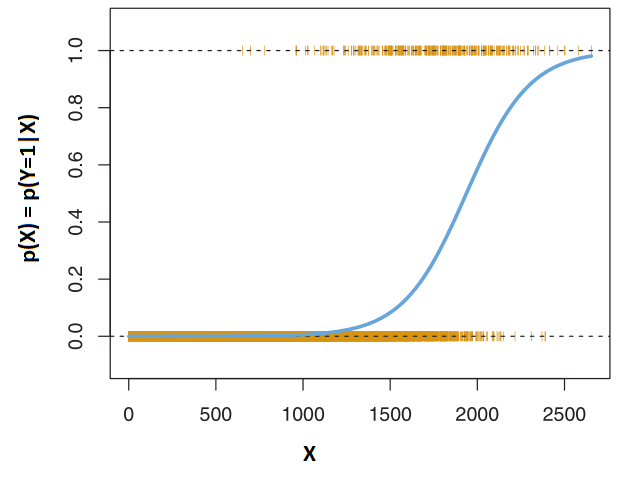
\includegraphics{img/lr_example.png}
\caption{}
\end{figure}

As for prediction, we use the model built with the estimated parameters
to predict probabilities. For example,

If \(X=1000\),

\[ \hat{p}(X) = \frac{e^{\hat{\beta_0} + \hat{\beta_1} X}}{1+e^{\hat{\beta_0} + \hat{\beta_1} X}} = \frac{e^{-10.6513+0.0055 \times 1000}}{1+e^{-10.6513+0.0055 \times 1000}} = 0.006\]

If \(X=2000\),

\[ \hat{p}(X) = \frac{e^{\hat{\beta_0} + \hat{\beta_1} X}}{1+e^{\hat{\beta_0} + \hat{\beta_1} X}} = \frac{e^{-10.6513+0.0055 \times 2000}}{1+e^{-10.6513+0.0055 \times 2000}} = 0.586\]

\section{Multiple Logistic
Regression}\label{multiple-logistic-regression}

We now consider the problem of predicting a binary response using
multiple predictors. By analogy with the extension from simple to
multiple linear regression in the previous chapters, we can generalize
the simple logistic regression equation as follows:

\[ \log( \frac{p(X)}{1-p(X)} ) = \beta_0 + \beta_1 X_1 +  \ldots + \beta_p X_p\]

where \(X=(X_1,\ldots,X_p)\) are \(p\) predictors. The equation above
can be rewritten as

\[ p(X) = \frac{e^{\beta_0 + \beta_1 X_1 +  \ldots + \beta_p X_p}}{1+e^{\beta_0 + \beta_1 X_1 +  \ldots + \beta_p X_p}} \]

Just as in the simple logistic regression we use the maximum likelihood
method to estimate \(\beta_0,\beta_1,\ldots,\beta_p\).

◼

\chapter*{PW 3}\label{pw-3}
\addcontentsline{toc}{chapter}{PW 3}

\section*{Report template}\label{report-template}
\addcontentsline{toc}{section}{Report template}

Create a new RMarkdown file and replace the YAML header with these
lines:

\begin{verbatim}
---
title: "Week 3"
subtitle: "Logistic Regression"
author: LastName FirstName
date: "23/01/2017"
output:
  html_document:
    toc: true
    toc_depth: 2
    toc_float: true
    theme: united
    highlight: zenburn
---
\end{verbatim}

Name the file \texttt{LastName\_FirstName\_Week3} and submit the html
output.

\section*{Social Networks Ads}\label{social-networks-ads}
\addcontentsline{toc}{section}{Social Networks Ads}

In this PW we are going to analyse the \texttt{Social\_Network\_Ads}
dataset. This dataset contains informations of users of a social
network. The social network has several business clients and its
business clients put ads on the social network for marketing compaigns
purposes. For this dataset, a company has put ads for one of its new
products and the social network gathered some informations about wich
users responded positively to the ad by buying the product and those who
responded negatively by not buying the product.

\textbf{1.} Download the \texttt{Social\_Network\_Ads} dataset from
\href{datasets/Social_Network_Ads.csv}{here} and import it into
\texttt{R}.

\textbf{2.} Describe the dataset (you can use \texttt{str()} and
\texttt{summary()} functions).

We will consider the variables \texttt{Age} and \texttt{EstimatedSalary}
as input variables (features) to see the correlations between them and
the decision of the user to buy (or not) the product.

\textbf{3.} Now we are going to split the dataset into training set and
test set. Last week we did it manually. From now on we will split it
randomly with this code,

\begin{Shaded}
\begin{Highlighting}[]
\KeywordTok{library}\NormalTok{(caTools) }\CommentTok{# install it first in the console}
\KeywordTok{set.seed}\NormalTok{(}\DecValTok{123}\NormalTok{)}
\CommentTok{# we use this function with the same number}
\CommentTok{# to randomly generate the same values}
\NormalTok{split =}\StringTok{ }\KeywordTok{sample.split}\NormalTok{(dataset$Purchased, }\DataTypeTok{SplitRatio =} \FloatTok{0.75}\NormalTok{)}
\CommentTok{# here we chose the SplitRatio to 75% of the dataset,}
\CommentTok{# and 25% for the test set.}
\NormalTok{training_set =}\StringTok{ }\KeywordTok{subset}\NormalTok{(dataset, split ==}\StringTok{ }\OtherTok{TRUE}\NormalTok{)}
\CommentTok{# we use subset to split the dataset}
\NormalTok{test_set =}\StringTok{ }\KeywordTok{subset}\NormalTok{(dataset, split ==}\StringTok{ }\OtherTok{FALSE}\NormalTok{)}
\end{Highlighting}
\end{Shaded}

\textbf{4.} Scale the input variables in both training set and test set.

First let us fit a simple logistic regression model of
\texttt{Purchased} in function of \texttt{Age}. We do it with this line
of code,

\begin{Shaded}
\begin{Highlighting}[]
\NormalTok{classifier <-}\StringTok{ }\KeywordTok{glm}\NormalTok{(Purchased ~}\StringTok{ }\NormalTok{Age , }\DataTypeTok{family =} \NormalTok{binomial, }\DataTypeTok{data=}\NormalTok{training_set)}
\CommentTok{# glm goes for generalized linear model}
\end{Highlighting}
\end{Shaded}

\textbf{5.} In the argument \texttt{family} of the function \texttt{glm}
we chose \texttt{binomial}. Why ?

\textbf{6.} What is the equation of the obtained model in the question
\textbf{4} ?

\textbf{7.} Is the feature \texttt{Age} significant?

\begin{rmdinsight}
The \textbf{AIC} is the \textbf{Akaike Information Criterion}. You will
use this while comparing multiple models. The model with lower value of
AIC is better. Suppose that we have a statistical model of some data.
Let \({\hat {L}}\) be the maximum value of the likelihood function for
the model; let \(k\) be the number of estimated parameters in the model.
Then the AIC value of the model is the following.

\[ \text{AIC} = 2 k-2 \ln(\hat{L})\]

where

\begin{itemize}
\tightlist
\item
  \(\hat{L}\) = the maximized value of the likelihood function of the
  model \(M\), i.e. \(\hat{L}=p(x|{\hat{\beta }},M)\), where
  \(\hat{\beta}\) are the parameter values that maximize the likelihood
  function.
\item
  \(x\) = the observed data.
\item
  \(k\) = the number of free parameters to be estimated. If the model
  under consideration is a linear regression, \(k\) is the number of
  regressors, including the intercept.
\end{itemize}
\end{rmdinsight}

\textbf{8.} Plot \texttt{Purchased} in function of \texttt{Age} and add
the curve of the obtained logistic regression model.

(\textbf{Hints}: First plot the point, then use the \texttt{curve()}
function with oprtion \texttt{add=TRUE} to add the curve to the plot.
The argument ``type'' of the function \texttt{predit()} must be
``reponse'')

You must obtain something like

\begin{figure}[htbp]
\centering
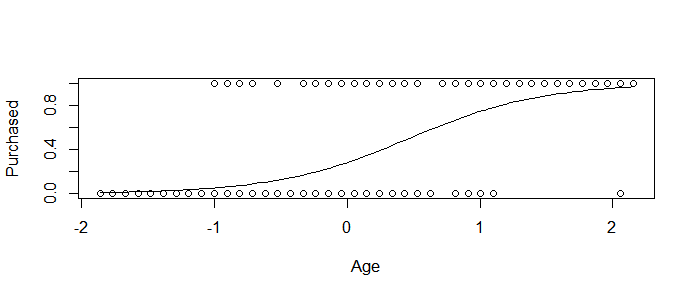
\includegraphics{img/glm1.png}
\caption{}
\end{figure}

\begin{rmdinsight}
\textbf{Extra}: A great R package for visualization if \texttt{ggplot2}.
Take a look on this
\href{http://www.r-graph-gallery.com/portfolio/ggplot2-package/}{link}
for some examples. With this library we obtain the following plot for
our model,

\begin{figure}[htbp]
\centering
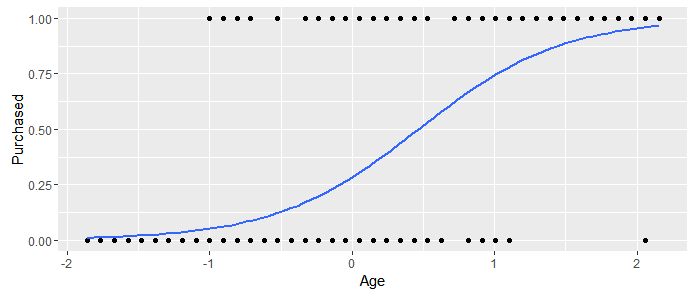
\includegraphics{img/glm_ggplot.png}
\caption{}
\end{figure}
\end{rmdinsight}

I obtained the last figure with these lines of code,

\begin{Shaded}
\begin{Highlighting}[]
\KeywordTok{library}\NormalTok{(ggplot2)}
\KeywordTok{ggplot}\NormalTok{(training_set, }\KeywordTok{aes}\NormalTok{(}\DataTypeTok{x=}\NormalTok{Age, }\DataTypeTok{y=}\NormalTok{Purchased)) +}
\StringTok{  }\KeywordTok{geom_point}\NormalTok{() +}
\StringTok{  }\KeywordTok{stat_smooth}\NormalTok{(}\DataTypeTok{method=}\StringTok{"glm"}\NormalTok{, }\DataTypeTok{method.args=}\KeywordTok{list}\NormalTok{(}\DataTypeTok{family=}\StringTok{"binomial"}\NormalTok{), }\DataTypeTok{se=}\OtherTok{FALSE}\NormalTok{)}
\end{Highlighting}
\end{Shaded}

\textbf{9.} Now let us take another feature into account in the model.
Fit a logistic regression model of purchasing the product in function of
the age of the user and its salary.

\textbf{10.} Are the predictors significant? Did the model get better by
adding t he estimated salary?

\textbf{11.} On the test set, predict the probability of purchasing the
product by the users using the obtained model.

\textbf{12.} Take a look on your predicted values for the variable
\texttt{Purchased}. We predicted the probability that the user will
purchase the product right? Now in order to compare your results with
the real answers, transform the predicted values to 0 or 1 (1 if
\textgreater{}0.5).

\textbf{Hint}: You can easily do it with the \texttt{ifelse()} function.

Now read the following about the evaluation of a classifier (of a
classification model).

\begin{rmdinsight}
\textbf{Confusion matrix}: is a tabular representation of Actual vs
Predicted values. This helps us to find the accuracy of the model. The
different results from a binary classifier are true positives, true
negatives, false positives, and false negatives. This is how the
confusion matrix looks like:

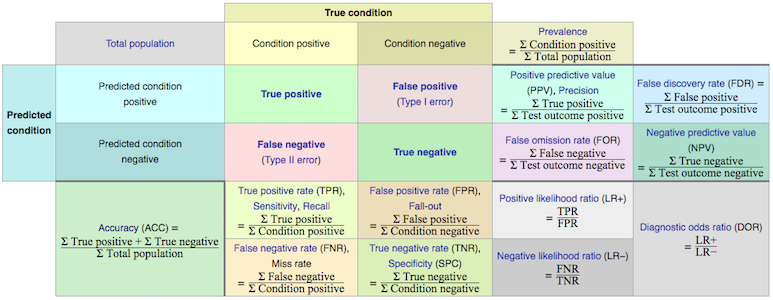
\includegraphics{img/cm.png} (Image source:
\href{https://en.wikipedia.org/wiki/Confusion_matrix}{Wikipedia})

You can calculate the \textbf{accuracy} of your model with:

\begin{figure}[htbp]
\centering
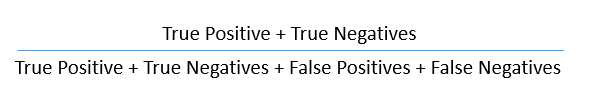
\includegraphics{img/cm1.png}
\caption{}
\end{figure}

\textbf{Accuracy} is a key measure of performance, and is more
specifically the rate at which the model is able to predict the correct
value (classification or regression) for a given data point or
observation. In other words, accuracy is the proportion of correct
predictions out of all predictions made.

The other two metrics from the confusion matrix worth discussing are
\textbf{precision} and \textbf{recall}. Precision (positive predictive
value) is the ratio of true positives to the total amount of positive
predictions made (i.e., true or false). Said another way, precision
measures the proportion of accurate positive predictions out of all
positive predictions made.

Recall on the other hand, or true positive rate, is the ratio of true
positives to the total amount of actual positives, whether predicted
correctly or not. So in other words, recall measures the proportion of
accurate positive predictions out of all actual positive observations.

A metric that is associated with precision and recall is called the
F-score (also called F1 score), which combines them mathematically, and
somewhat like a weighted average, in order to produce a single measure
of performance based on the simultaneous values of both. Its values
range from 0 (worst) to 1 (best).

Another important concept to know about is the \textbf{\emph{Receiver
Operating Characteristic}}, which when plotted, results in what's known
as an ROC curve.

\textbf{ROC Curve}: An ROC curve is a two-dimensional plot of
\emph{sensitivity} (recall, or true positive rate) vs \emph{specificity}
(false positive rate). The area under the curve is referred to as the
\textbf{\emph{AUC}}, and is a numeric metric used to represent the
quality and performance of the classifier (model).

\begin{figure}[htbp]
\centering
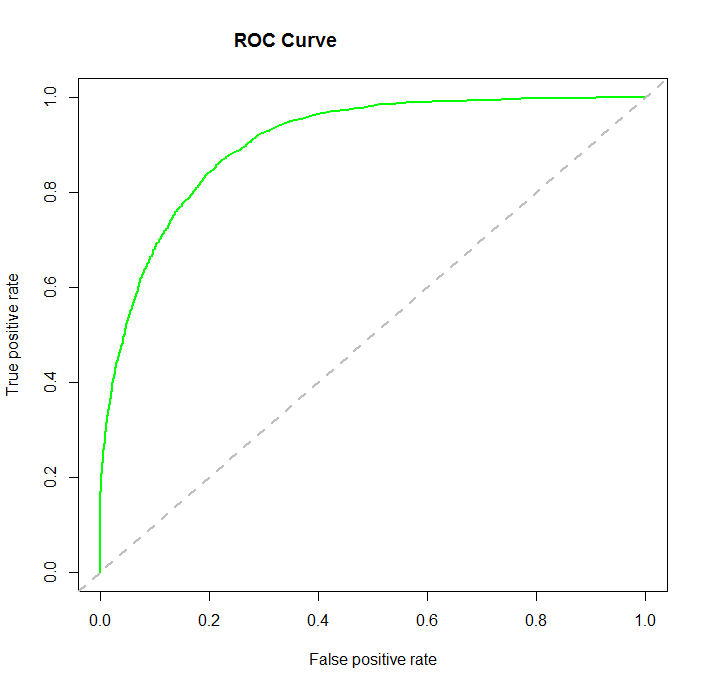
\includegraphics{img/roc.png}
\caption{}
\end{figure}

An AUC of 0.5 is essentially the same as random guessing without a
model, whereas an AUC of 1.0 is considered a perfect classifier.
Generally, the higher the AUC value the better, and an AUC above 0.8 is
considered quite good.

The higher the AUC value, the closer the curve gets to the upper left
corner of the plot. One can easily see from the ROC curves then that the
goal is to find and tune a model that maximizes the true positive rate,
while simultaneously minimizing the false positive rate. Said another
way, the goal as shown by the ROC curve is to correctly predict as many
of the actual positives as possible, while also predicting as many of
the actual negatives as possible, and therefore minimize errors
(incorrect classifications) for both.
\end{rmdinsight}

\textbf{13.} Now to evaluate the predictions, compute the confusion
matrix. What do you obtain ?

(\textbf{Hint}: you can use the \texttt{table()} function).

\textbf{14.} Calculate the accuracy, specificity, sensitivity and the
precision of the model.

\textbf{15.} Plot the ROC curve and calculate AUC value.

\begin{rmdinsight}
\textbf{Hints}: to plot it, install the \texttt{ROCR} package. Load and
use the functions:

\begin{itemize}
\tightlist
\item
  \texttt{prediction()} to calculate the elements of the confusion
  matrix.
\item
  \texttt{performance()} to calculate the AUC.
\item
  \texttt{plot()} to plot the ROC curve, you can plot the performance
  calculated before.
\item
  \texttt{abline()} to plot a line of equation \texttt{y=x}.
\end{itemize}
\end{rmdinsight}

\textbf{16.} Compare the AUC of the two models you fitted (one with only
age and one with age and estimated salary) and plot their ROC curves in
the same figure.

◼

\chapter{Linear Discriminant
Analysis}\label{linear-discriminant-analysis}

Discriminant analysis is a popular method for multiple-class
classification. We will start first by the \emph{Linear Discriminant
Analysis (LDA)}.

\section{Introduction}\label{introduction-2}

As we saw in the previous chapter, Logistic regression involves directly
modeling \(\mathbb{P} (Y = k|X = x)\) using the \emph{logistic
function}, for the case of two response classes. In logistic regression,
we model the conditional distribution of the response \(Y\), given the
predictor(s) \(X\). We now consider an alternative and less direct
approach to estimating these probabilities. In this alternative
approach, \textbf{\emph{we model the distribution}} of the predictors
\(X\) \textbf{\emph{separately}} in each of the response classes
(i.e.~given \(Y\)), and then use \textbf{Bayes' theorem} to flip these
around into estimates for \(\mathbb{P} (Y = k|X = x)\). When these
distributions are assumed to be \emph{Normal}, it turns out that the
model is very similar in form to logistic regression.

\textbf{Why not logistic regression?} Why do we need another method,
when we have logistic regression? There are several reasons:

\begin{itemize}
\tightlist
\item
  When the classes are well-separated, the parameter estimates for the
  logistic regression model are surprisingly unstable. Linear
  discriminant analysis does not suffer from this problem.
\item
  If \(n\) is small and the distribution of the predictors \(X\) is
  approximately normal in each of the classes, the linear discriminant
  model is again more stable than the logistic regression model.
\item
  Linear discriminant analysis is popular when we have \emph{more than
  two response classes}.
\end{itemize}

\section{Bayes' Theorem}\label{bayes-theorem}

Bayes' theorem is stated mathematically as the following equation:

\[ P(A | B) = \frac{P(A \cap B)}{P(B)} =  \frac{P(B|A) P(A)}{P(B)}\]

where \(A\) and \(B\) are events and \(P(B) \neq 0\).

\begin{itemize}
\tightlist
\item
  \(P(A | B)\), a conditional probability, is the probability of
  observing event \(A\) given that \(B\) is true. It is called the
  \textbf{\emph{posterior}} probability.
\item
  \(P(A)\), is called the \textbf{\emph{prior}}, is the initial degree
  of belief in A.
\item
  \(P(B)\) is the \textbf{\emph{likelihood}}.
\end{itemize}

\begin{rmdinsight}
The posterior probability can be written in the memorable form as :

Posterior probability \(\propto\) Likelihood \(\times\) Prior
probability.
\end{rmdinsight}

\textbf{Extended form}:

Suppose we have a partition \(\{A_i\}\) of the sample space, the even
space is given or conceptualized in terms of \(P(A_j)\) and
\(P(B | A_j)\). It is then useful to compute \(P(B)\) using the law of
total probability:

\[ P(B) = \sum_j P(B|A_j) P(A_j) \]

\[ \Rightarrow P(A_i|B) = \frac{P(B|A_i) P(A_i)}{\sum_j P(B|A_j) P(A_j)} \]

\textbf{Bayes' Theorem for Classification}:

Suppose that we wish to classify an observation into one of \(K\)
classes, where \(K \geq 2\). In other words, the qualitative response
variable \(Y\) can take on \(K\) possible distinct and unordered values.

Let \(\pi_k\) represent the overall or \emph{prior} probability that a
randomly chosen observation comes from the \(k\)-th class; this is the
probability that a given observation is associated with the \(k\)-th
category of the response variable \(Y\).

Let \(f_k(X) \equiv P(X = x|Y = k)\) denote the \emph{density function}
of \(X\) for an observation that comes from the \(k\)-th class. In other
words, \(f_k(x)\) is relatively large if there is a high probability
that an observation in the \(k\)-th class has \(X \approx x\), and
\(f_k(x)\) is small if it is very unlikely that an observation in the
\(k\)-th class has \(X \approx x\). Then \emph{Bayes' theorem} states
that

\begin{equation}
P(Y=k|X=x) = \frac{ \pi_k f_k(x)}{\sum_{c=1}^K \pi_c f_c(x)}
\label{eq:bayes}
\end{equation}

As we did in the last chapter, we will use the abbreviation
\(p_k(X) =P(Y = k|X)\).

The equation above stated by \emph{Bayes' theorem} suggests that instead
of directly computing \(p_k(X)\) as we did in the logistic regression,
we can simply plug in estimates of \(\pi_k\) and \(f_k(X)\) into the
equation. In general, estimating \(\pi_k\) is easy (the fraction of the
training observations that belong to the \(k\)-th class). But estimating
\(f_k(X)\) tends to be more challenging.

\begin{quote}
Recall that \(p_k(x)\) is the \emph{posterior} probability that an
observation \(X=x\) belongs to \(k\)-th class.
\end{quote}

\begin{quote}
If we can find a way to estimate \(f_k(X)\), we can develop a classifier
with the lowest possibe error rate out of all classifiers.
\end{quote}

\section{\texorpdfstring{LDA for
\(p=1\)}{LDA for p=1}}\label{lda-for-p1}

Assume that \(p=1\), which mean we have only one predictor. We would
like to obtain an estimate for \(f_k(x)\) that we can plug into the
Equation \eqref{eq:bayes} in order to estimate \(p_k(x)\). \textbf{We will
then classify an observation to the class for which \(p_k(x)\) is
greatest}.

In order to estimate \(f_k(x)\), we will first make some assumptions
about its form.

Suppose we assume that \(f_k(x)\) is \emph{normal} (\emph{Gaussian}). In
the one-dimensional setting, the normal density take the form

\begin{equation}
f_k(x)= \frac{1}{\sigma_k\sqrt{2\pi}} \exp \big( - \frac{1}{2\sigma_k^2 } (x-\mu_k)^2\big)
\label{eq:normal01}
\end{equation}

where \(\mu_k\) and \(\sigma_k^2\) are the mean and variance parameters
for \(k\)-th class. Let us assume that
\(\sigma_1^2 = \ldots = \sigma_K^2 = \sigma\) (which means there is a
shared variance term across all \(K\) classes). Plugging Eq.
\eqref{eq:normal01} into the Bayes formula in Eq. \eqref{eq:bayes} we get,

\begin{equation}
p_k(x) = \frac{  \pi_k \frac{1}{\sigma \sqrt{2\pi}} e^{-\frac{1}{2} \big(\frac{x-\mu_k}{\sigma}\big)^2 } }{  \sum_{c=1}^K  \pi_c \frac{1}{\sigma \sqrt{2\pi}} e^{-\frac{1}{2} \big(\frac{x-\mu_c}{\sigma}\big)^2 } }
\label{eq:pkx}
\end{equation}

\begin{rmdcaution}
Note that \(\pi_k\) and \(\pi_c\) denote the prior probabilities. And
\(\pi\) is the mathematical constant \(\pi \approx 3.14159\).
\end{rmdcaution}

To classify at the value \(X = x\), we need to see which of the
\(p_k(x)\) is largest. Taking logs, and discarding terms that do not
depend on \(k\), we see that this is equivalent to assigning \(x\) to
the class with the largest \textbf{\emph{discriminant score}}:

\begin{equation}
\delta_k(x) = x.\frac{\mu_k}{\sigma^2} - \frac{\mu_k^2}{2\sigma^2} + \log (\pi_k)
\label{eq:discscore}
\end{equation}

Note that \(\delta_k(x)\) is a \emph{linear} function of \(x\).

\begin{rmdinsight}
\begin{itemize}
\tightlist
\item
  The decision surfaces for a linear discriminant classifiers are
  defined by the linear equations \(\delta_k(x) = \delta_c(x)\).
\item
  Example: If \(K=2\) and \(\pi_1=\pi_2\), then the \textbf{desicion
  boundary} is at \(x=\frac{\mu_1+\mu2}{2}\) (\textbf{Prove it!}).
\item
  An example where \(\mu_1=-1.5\), \(\mu_2=1.5\), \(\mu_1=\mu_2=0.5\)
  and \(\sigma^2=1\) is shown in this following figure
\end{itemize}

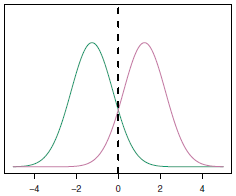
\includegraphics{img/decbound.png}

\begin{itemize}
\item
  See this
  \href{https://www.coursera.org/learn/machine-learning/lecture/WuL1H/decision-boundary}{video}
  to understand more about \emph{decision boundary}.
\item
  As we classify a new point according to which density is highest, when
  the priors are different we take them into account as well, and compare
  \(\pi_k f_k(x)\). On the right of the following figure, we favor the
  pink class (remark that the decision boundary has shifted to the
  left).
\end{itemize}

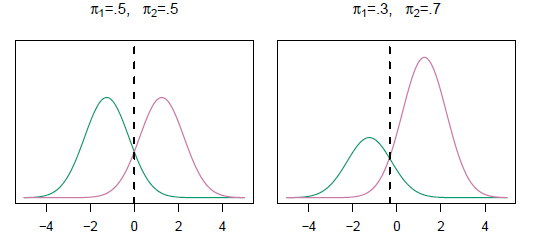
\includegraphics{img/decbound2.png}
\end{rmdinsight}

\section{Estimating the parameters}\label{estimating-the-parameters}

Typically we don't know these parameters; we just have the training
data. In that case we simply estimate the parameters and plug them into
the rule.

Let \(n\) the total number of training observations, and \(n_k\) the
number of training observations in the \(k\)-th class. The following
estimates are used:

\begin{align*}
\hat{\pi}_k &= \frac{n_k}{n} \\
\hat{\mu}_k &= \frac{1}{n_k} \sum_{i: y_i=k} x_i \\
\hat{\sigma}^2 &= \frac{1}{n - K} \sum_{k=1}^K \sum_{i: y_i=k} (x_i-\hat{\mu}_k)^2 \\
 &= \sum_{k=1}^K \frac{n_k-1}{n - K} . \hat{\sigma}_k^2
\end{align*}

where
\(\hat{\sigma}_k^2 = \frac{1}{n_k-1}\sum_{i: y_i=k}(x_i-\hat{\mu}_k)^2\)
is the usual formula for the estimated variance in the -\(k\)-th class.

The linear discriminant analysis (LDA) classifier plugs these estimates
in Eq. \eqref{eq:discscore} and assigns an observation \(X=x\) to the
class for which

\begin{equation}
\hat{\delta}_k(x) = x.\frac{\hat{\mu}_k}{\hat{\sigma}^2} - \frac{\hat{\mu}_k^2}{2\hat{\sigma}^2} + \log (\hat{\pi}_k)
\label{eq:discscoreest}
\end{equation}

is largest.

The \emph{discriminant functions} in Eq. \eqref{eq:discscoreest} are
linear functions of \(x\).

\begin{quote}
Recall that we assumed that the observations come from a normal
distribution with a common variance \(\sigma^2\).
\end{quote}

\section{\texorpdfstring{LDA for
\(p > 1\)}{LDA for p \textgreater{} 1}}\label{lda-for-p-1}

Let us now suppose that we have multiple predictors. We assume that
\(X=(X_1,X_2,\ldots,X_p)\) is drawn from \emph{multivariate Gaussian}
distribution (assuming they have a common covariance matrix, e.g.~same
variances as in the case of \(p=1\)). The multivariate Gaussian
distribution assumes that each individual predictor follows a
one-dimensional normal distribution as in Eq. \eqref{eq:normal01}, with
some correlation between each pair of predictors.

To indicate that a \(p\)-dimensional random variable \(X\) has a
multivariate Gaussian distribution, we write
\(X \sim \mathcal{N}(\mu,\Sigma)\). Where

\[ \mu = E(X) = \begin{pmatrix}
    \mu_1 \\
    \mu_2 \\
    \vdots \\
    \mu_p
\end{pmatrix} \]

and, \[ \Sigma = Cov(X) = \begin{pmatrix}
    \sigma_1^2 & Cov[X_1, X_2]  & \dots  & Cov[X_1, X_p] \\
    Cov[X_2, X_1] & \sigma_2^2  & \dots  & Cov[X_2, X_p] \\
    \vdots & \vdots &  \ddots & \vdots \\
    Cov[X_p, X_1] & Cov[X_p, X_2]  & \dots  & \sigma_p^2
\end{pmatrix}  \]

\begin{quote}
\(\Sigma\) is the \(p\times p\) covariance matrix of \(X\).
\end{quote}

Formally, the multivariate Gaussian density is defined as

\[f(x) = \frac{1}{(2\pi)^{p/2} |\Sigma|^{1/2}} \exp \bigg( - \frac{1}{2} (x-\mu)^T \Sigma^{-1} (x-\mu) \bigg)
\]

Plugging the density function for the \(k\)-th class, \(f_k(X=x)\), into
Eq. \eqref{eq:bayes} reveals that the Bayes classifier assigns an
observation \(X=x\) to the class for which

\begin{equation}
\delta_k(x) = x^T \Sigma^{-1} \mu_k - \frac{1}{2} \mu_k^T \Sigma^{-1}  \mu_k + \log \pi_k
\label{eq:discscorematrix}
\end{equation}

is largest. This is the vector/matrix version of \eqref{eq:discscore}.

An example is shown in the following figure. Three equally-sized
Gaussian classes are shown with class-specific mean vectors and a common
covariance matrix (\(\pi_1=\pi_2=\pi_3=1/3\)). The three ellipses
represent regions that contain \(95\%\) of the probability for each of
the three classes. The dashed lines are the Bayes decision boundaries.

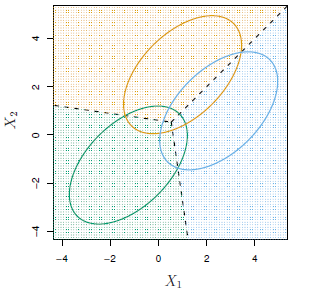
\includegraphics{img/lda2.png}

Recall that the decision boundaries represent the set of values \(x\)
for which \(\delta_k(x)=\delta_c(x)\); i.e.~for \(k\neq c\)

\[ x^T \Sigma^{-1} \mu_k - \frac{1}{2} \mu_k^T \Sigma^{-1}  \mu_k = x^T \Sigma^{-1} \mu_c - \frac{1}{2} \mu_c^T \Sigma^{-1}  \mu_c  \]

Note that there are three lines representing the Bayes decision
boundaries because there are three pairs of classes among the three
classes. That is, one Bayes decision boundary separates class 1 from
class 2, one separates class 1 from class 3, and one separates class 2
from class 3. These three Bayes decision boundaries divide the predictor
space into three regions. The Bayes classifier will classify an
observation according to the region in which it is located.

Once again, we need to estimate the unknown parameters
\(\mu_1,\ldots,\mu_k,\) and \(\pi_1,\ldots,\pi_k,\) and \(\Sigma\); the
formulas are similar to those used in the one-dimensional case. To
assign a new observation \(X = x\), LDA plugs these estimates into Eq.
\eqref{eq:discscorematrix} and classifies to the class for which
\(\delta_k(x)\) is largest.

Note that in Eq. \eqref{eq:discscorematrix} \(\delta_k(x)\) is a
\emph{linear} function of \(x\); that is, the LDA decision rule depends
on x only through a linear combination of its elements. This is the
reason for the word linear in LDA.

\section{Making predictions}\label{making-predictions}

Once we have estimates \(\hat{\delta}_k(x)\), we can turn these into
estimates for class probabilities:

\[ \hat{P}(Y=k|X=x)= \frac{e^{\hat{\delta}_k(x)}}{\sum_{c=1}^K e^{\hat{\delta}_c(x)}} \]

So classifying to the largest \(\hat{\delta}_k(x)\) amounts to
classifying to the class for which \(\hat{P}(Y=k|X=x)\) is largest.

When \(K=2\), we classify to class 2 if \(\hat{P}(Y=2|X=x) \geq 0.5\),
else to class 1.

\section{Other forms of Discriminant
Analysis}\label{other-forms-of-discriminant-analysis}

\[P(Y=k|X=x) = \frac{ \pi_k f_k(x)}{\sum_{c=1}^K \pi_c f_c(x)}\]

We saw before that when \(f_k(x)\) are Gaussian densities, whith the
same covariance matrix \(\Sigma\) in each class, this leads to Linear
Discriminant Analysis (LDA).

By altering the forms for \(f_k(x)\), we get different classifiers.

\begin{itemize}
\tightlist
\item
  With Gaussians but different \(\Sigma_k\) in each class, we get
  \emph{Quadratic Discriminant Analysis (QDA)}.
\item
  With \(f_k(x) = \prod_{j=1}^p f_{jk}(x_j)\) (conditional independence
  model) in each class we get \emph{Naive Bayes}. (For Gaussian, this
  mean the \(\Sigma_k\) are diagonal, e.g.
  \(Cov(X_i,X_j)=0 \,\, \forall \, \, 1\leq i,j \leq p\)).
\item
  Many other forms by proposing specific density models for \(f_k(x)\),
  including \emph{nonparametric approaches}.
\end{itemize}

\subsection{Quadratic Discriminant Analysis
(QDA)}\label{quadratic-discriminant-analysis-qda}

Like LDA, the QDA classifier results from assuming that the observations
from each class are drawn from a Gaussian distribution, and plugging
estimates for the parameters into Bayes' theorem in order to perform
prediction.

However, unlike LDA, QDA assumes that each class has its own covariance
matrix. Under this assumption, the Bayes classifier assigns an
observation \(X = x\) to the class for which

\begin{align*}
\delta_k(x) &= - \frac{1}{2} (x-\mu)^T \Sigma_k^{-1} (x-\mu) - \frac{1}{2} \log |\Sigma_k| + \log \pi_k \\
            &= - \frac{1}{2} x^T \Sigma_k^{-1} x + \frac{1}{2} x^T \Sigma_k^{-1} \mu_k - \frac{1}{2} \mu_k^T \Sigma_k^{-1} \mu_k - \frac{1}{2} \log |\Sigma_k| + \log \pi_k
\end{align*}

is largest.

Unlike in LDA, the quantity \(x\) appears as a quadratic function in
QDA. This is where QDA gets its name.

\begin{rmdcaution}
The decision boundary in QDA is non-linear. It is quadratic (a curve).
\end{rmdcaution}

\subsection{Naive Bayes}\label{naive-bayes}

We use Naive Bayes classifier if the features are independant in each
class. It is useful when \(p\) is large (unklike LDA and QDA).

Naive Bayes assumes that each \(\Sigma_k\) is diagonal, so

\begin{align*}
\delta_k(x) &\propto \log \bigg[\pi_k \prod_{j=1}^p f_{kj}(x_j) \bigg] \\
            &= -\frac{1}{2} \sum_{j=1}^p \frac{(x_j-\mu_{kj})^2}{\sigma_{kj}^2} + \log \pi_k
\end{align*}

It can used for mixed feature vectors (qualitative and quantitative). If
\(X_j\) is qualitative, we replace \(f_{kj}(x_j)\) by probability mass
function (histogram) over discrete categories.

\section{LDA vs Logistic Regression}\label{lda-vs-logistic-regression}

the logistic regression and LDA methods are closely connected. Consider
the two-class setting with \(p =1\) predictor, and let \(p_1(x)\) and
\(p_2(x)=1−p_1(x)\) be the probabilities that the observation \(X = x\)
belongs to class 1 and class 2, respectively. In the LDA framework, we
can see from Eq. \eqref{eq:discscore} (and a bit of simple algebra) that
the log odds is given by

\[ \log \bigg(\frac{p_1(x)}{1-p_1(x)}\bigg) = \log \bigg(\frac{p_1(x)}{p_2(x)}\bigg) = c_0 + c_1 x\]

where \(c_0\) and \(c_1\) are functions of \(\mu_1, \mu_2,\) and
\(\sigma^2\).

On the other hand, we know that in logistic regression

\[ \log \bigg(\frac{p_1}{1-p_1}\bigg) = \beta_0 + \beta_1 x\]

Both of the equations above are linear functions of \(x\). Hence both
logistic regression and LDA produce linear decision boundaries. The only
difference between the two approaches lies in the fact that \(\beta_0\)
and \(\beta_1\) are estimated using \emph{maximum likelihood}, whereas
\(c_0\) and \(c_1\) are computed using the estimated mean and variance
from a \emph{normal distribution}. This same connection between LDA and
logistic regression also holds for multidimensional data with \(p> 1\).

\begin{rmdinsight}
\begin{itemize}
\tightlist
\item
  Logistic regression uses the conditional likelihood based on
  \(P(Y|X)\) (known as \emph{discriminative learning}).
\item
  LDA uses the full likelihood based on \(P(X,Y )\) (known as
  \emph{generative learning}).
\item
  Despite these differences, in practice the results are often very
  similar.
\end{itemize}

\textbf{Remark}: Logistic regression can also fit quadratic boundaries
like QDA, by explicitly including quadratic terms in the model.
\end{rmdinsight}

◼

\chapter*{PW 4}\label{pw-4}
\addcontentsline{toc}{chapter}{PW 4}

This week we are going to continue the analysis of the
\texttt{Social\_Network\_Ads} dataset. Recall that this dataset contains
informations of users of a social network and if they bought a specified
product. Last week we built a Logistic Regression model for the variable
\texttt{Purchased} in function of \texttt{Age} and
\texttt{EstimatedSalary}. We will consider the same variables this week
but we will fit different models using methods such as LDA, QDA, and
Naive Bayes.

\section*{Report template}\label{report-template-1}
\addcontentsline{toc}{section}{Report template}

For this week, use these YAML settings for your RMarkdown file:

\begin{verbatim}
---
title: "Week 4"
subtitle: "Discriminant Analysis"
author: LastName FirstName
date: "30/01/2017"
output:
  html_document:
    toc: true
    toc_depth: 2
    toc_float: true
    theme: cerulean
    highlight: espresso
---
\end{verbatim}

\section*{Decision Boundary of Logistic
Regression}\label{decision-boundary-of-logistic-regression}
\addcontentsline{toc}{section}{Decision Boundary of Logistic Regression}

\textbf{1.} First, re-do the pre-processing steps you did last week
(remove the first two columns from the dataset as we are not going to
use them) and fit a logistic regression model of \texttt{Purchased} in
function of \texttt{Age} and \texttt{EstimatedSalary}. Name your model
\texttt{classifier.logreg}. If you need the dataset again, you can
download it from \href{datasets/Social_Network_Ads.csv}{here}.

Now you are going to visualize the decision boundary for logistic
regression.

\begin{rmdinsight}
\begin{itemize}
\tightlist
\item
  Since the decision boundary of logistic regression is a linear
  (\emph{you know why right?}) and the dimension of the feature space is
  2 (\texttt{Age} and \texttt{EstimatedSalary}), the decision boundary
  in this 2-dimensional space is a line that separates the predicted
  classes ``0'' and ``1'' (values of the response \texttt{Purchased}).
\item
  For logistic regression, we predict \(y=1\) if \(\beta^T X \geq 0\)
  (right side of the line) and \(y=0\) if \(\beta^T X < 0\) (left side
  of the line). Where
\end{itemize}

\[ \beta = \begin{pmatrix} \beta_0 \\ \beta_1 \\ \beta2 \end{pmatrix} \,\, \text{and} \,\, X = \begin{pmatrix}
  1 \\
  X_1 \\
  X_2
  \end{pmatrix}\]

So we predict \(y=1\) if \(\beta_0 + \beta_1 X_1 + \beta_2 X_2 \geq 0\)
which means that the equation of the decision boundary (a line here) is
\(X_2 = - \frac{\beta_1}{\beta_2}X_1 - \frac{\beta_0}{\beta_2}\)
\end{rmdinsight}

\textbf{2.} Plot the decision boundary obtained with logistic
regression. In order to do so, calculate the intercept and the slope of
the line presenting the decision boundary, then plot
\texttt{EstimatedSalary} in function of \texttt{Age} (from the
\texttt{test\_set}) and add the line using \texttt{abline()}.

\textbf{3.} In order to verify that your line (decision boundary) is
well plotted, color the points on the last Figure with respect to the
predicted response.

\textbf{Hints}:

\begin{itemize}
\tightlist
\item
  If your predictions are stored in \texttt{y\_pred}, you can do it
  using
  \texttt{bg\ =\ ifelse(y\_pred\ ==\ 1,\ \textquotesingle{}color1\textquotesingle{},\ \textquotesingle{}color2\textquotesingle{})},
  and precise the argument \texttt{pch} to be 21 (you can choose pch to
  be a value between 21 and 25, try it).
\item
  Then, add the line using \texttt{abline()}, put the line width = 2 to
  make it more visible. Do not forget to title the Figure).
\end{itemize}

\textbf{4.} Now make the same plot but color the points with respect to
their real labels (the variable \texttt{Purchased}). From this figure,
count the number of the false positive predictions and compare it to the
value obtained in the confusion matrix.

\section*{Linear Discriminant Analysis
(LDA)}\label{linear-discriminant-analysis-lda}
\addcontentsline{toc}{section}{Linear Discriminant Analysis (LDA)}

Let us apply linear discriminant analysis (LDA) now. First we will make
use of the \texttt{lda()} function in the package \texttt{MASS}. Second,
you are going to create the model and predict the classes by yourself
without using the \texttt{lda()} function. And we will visualize the
decision boundary of LDA.

\textbf{5.} Fit a LDA model of \texttt{Purchased} in function of
\texttt{Age} and \texttt{EstimatedSalary}. Name the model
\texttt{classifier.lda}.

\begin{Shaded}
\begin{Highlighting}[]
\KeywordTok{library}\NormalTok{(MASS)}
\NormalTok{classifier.lda <-}\StringTok{ }\KeywordTok{lda}\NormalTok{(Purchased~Age+EstimatedSalary, }\DataTypeTok{data=}\NormalTok{training_set)}
\end{Highlighting}
\end{Shaded}

\textbf{6.} Call \texttt{classifier.lda} and see what does it compute.

\textbf{Plus:} If you enter the following you will be returned with a
list of summary information concerning the computation:

\begin{Shaded}
\begin{Highlighting}[]
\NormalTok{classifier.lda$prior}
\NormalTok{classifier.lda$means}
\end{Highlighting}
\end{Shaded}

\textbf{7.} On the test set, predict the probability of purchasing the
product by the users using the model \texttt{classifier.lda}. Remark
that when we predict using LDA, we obtain a list instead of a matrix, do
\texttt{str()} for your predictions to see what do you get.

\textbf{Remark}: we get the predicted class here, without being
obligated to round the predictions as we did for logistic regression.

\textbf{8.} Compute the confusion matrix and compare the predictions
results obtained by LDA to the ones obtained by logistic regression.
What do you remark?

(\textbf{Hint}: compare the accuracy)

\textbf{9.} Now let us plot the decision boundary obtained with LDA. You
saw in the course that decision boundary for LDA represent the set of
values \(x\) where \(\delta_k(x) = \delta_c(x)\). Recall that
\[ \delta_k(X) = x^T \Sigma^{-1} \mu_k - \frac{1}{2} \mu_k^T \Sigma^{-1}  \mu_k + \log \pi_k \]

Here in our case, we have 2 classes (\(K=2\)) and 2 predictors
(\(p=2\)). So the decision boundary (which is linear in the case of LDA,
and line in our case since \(p=2\)) will verify the equation
\(\delta_0(x) = \delta_1(x)\) Since we have two classes ``0'' and ``1''.
In the case of LDA this leads to linear boundary and is easy to be
plotted. But in more complicated cases it is difficult to manually
simplify the equations and plot the decision boundary. Anyway, there is
a smart method to plot (but a little bit costy) the decision boundary in
\texttt{R} using the function \texttt{contour()}, the corresponding code
is the following (you must adapt it and use it to plot your decision
boundary):

\begin{Shaded}
\begin{Highlighting}[]
\CommentTok{# create a grid corresponding to the scales of Age and EstimatedSalary}
\CommentTok{# and fill this grid with lot of points}
\NormalTok{X1 =}\StringTok{ }\KeywordTok{seq}\NormalTok{(}\KeywordTok{min}\NormalTok{(training_set[, }\DecValTok{1}\NormalTok{]) -}\StringTok{ }\DecValTok{1}\NormalTok{, }\KeywordTok{max}\NormalTok{(training_set[, }\DecValTok{1}\NormalTok{]) +}\StringTok{ }\DecValTok{1}\NormalTok{, }\DataTypeTok{by =} \FloatTok{0.01}\NormalTok{)}
\NormalTok{X2 =}\StringTok{ }\KeywordTok{seq}\NormalTok{(}\KeywordTok{min}\NormalTok{(training_set[, }\DecValTok{2}\NormalTok{]) -}\StringTok{ }\DecValTok{1}\NormalTok{, }\KeywordTok{max}\NormalTok{(training_set[, }\DecValTok{2}\NormalTok{]) +}\StringTok{ }\DecValTok{1}\NormalTok{, }\DataTypeTok{by =} \FloatTok{0.01}\NormalTok{)}
\NormalTok{grid_set =}\StringTok{ }\KeywordTok{expand.grid}\NormalTok{(X1, X2)}
\CommentTok{# Adapt the variable names}
\KeywordTok{colnames}\NormalTok{(grid_set) =}\StringTok{ }\KeywordTok{c}\NormalTok{(}\StringTok{'Age'}\NormalTok{, }\StringTok{'EstimatedSalary'}\NormalTok{)}

\CommentTok{# plot 'Estimated Salary' ~ 'Age'}
\KeywordTok{plot}\NormalTok{(test_set[, -}\DecValTok{3}\NormalTok{],}
     \DataTypeTok{main =} \StringTok{'Decision Boundary LDA'}\NormalTok{,}
     \DataTypeTok{xlab =} \StringTok{'Age'}\NormalTok{, }\DataTypeTok{ylab =} \StringTok{'Estimated Salary'}\NormalTok{,}
     \DataTypeTok{xlim =} \KeywordTok{range}\NormalTok{(X1), }\DataTypeTok{ylim =} \KeywordTok{range}\NormalTok{(X2))}

\CommentTok{# color the plotted points with their real label (class)}
\KeywordTok{points}\NormalTok{(test_set, }\DataTypeTok{pch =} \DecValTok{21}\NormalTok{, }\DataTypeTok{bg =} \KeywordTok{ifelse}\NormalTok{(test_set[, }\DecValTok{3}\NormalTok{] ==}\StringTok{ }\DecValTok{1}\NormalTok{, }\StringTok{'green4'}\NormalTok{, }\StringTok{'red3'}\NormalTok{))}

\CommentTok{# Make predictions on the points of the grid, this will take some time}
\NormalTok{pred_grid =}\StringTok{ }\KeywordTok{predict}\NormalTok{(classifier.lda, }\DataTypeTok{newdata =} \NormalTok{grid_set)$class}

\CommentTok{# Separate the predictions by a contour}
\KeywordTok{contour}\NormalTok{(X1, X2, }\KeywordTok{matrix}\NormalTok{(}\KeywordTok{as.numeric}\NormalTok{(pred_grid), }\KeywordTok{length}\NormalTok{(X1), }\KeywordTok{length}\NormalTok{(X2)), }\DataTypeTok{add =} \OtherTok{TRUE}\NormalTok{)}
\end{Highlighting}
\end{Shaded}

\textbf{10.} Now let us build a LDA model for our data set without using
the \texttt{lda()} function. You are free to do it by creating a
function or without creating one. Go back to question \textbf{6} and see
what did you obtain by using \texttt{lda()}. It computes the prior
probability of group membership and the estimated group means for each
of the two groups. Additional information that is not provided, but may
be important, is the single covariance matrix that is being used for the
various groupings.

\begin{rmdinsight}
In LDA, we compute for every observation \(x\) its discriminant score
\(\delta_k(x)\). Then we attribute \(x\) to the class that has the
highest \(\delta\). Recall that

\[\delta_k(x) = x^T \Sigma^{-1} \mu_k - \frac{1}{2} \mu_k^T \Sigma^{-1}  \mu_k + \log \pi_k\]

So to compute \(\delta_k(x)\) we need to estimate \(\pi_k\), \(\mu_k\)
and \(\Sigma\).

Note that \[x=\begin{pmatrix}
            X_1 \\
            X_2
            \end{pmatrix}\] and here \(X_1\)=\texttt{Age} and
\(X_2\)=\texttt{EstimatedSalary}.
\end{rmdinsight}

So let us do it step by step, first we will do the estimates:

\textbf{10.1} Subset the training set into two sets: \texttt{class0}
where \texttt{Purchased\ =\ 0} and \texttt{class1} where
\texttt{Purchased\ =\ 1}).

\textbf{10.2} Compute \(\pi_0\) and \(\pi_1\).

\[\pi_i = N_i / N, \,\, \text{where} \,\, N_i \,\, \text{is the number of data points in group } i\]

\textbf{10.3} Compute \(\mu_0\) and \(\mu_1\). \[\mu_0 = \begin{pmatrix}
   \mu_0(X_1) \\
   \mu_0(X_2)
   \end{pmatrix} \,\, \text{and} \,\, \mu_1 = \begin{pmatrix}
   \mu_1(X_1) \\
   \mu_1(X_2)
   \end{pmatrix}\]

where, for example, \(\mu_0(X_1)\) is the mean of the variable \(X_1\)
in the group \(0\) (the subset \texttt{class0}).

\textbf{10.4} Compute \(\Sigma\). In the case of two classes like here,
it is computed by calculating the following:

\[\Sigma = \frac{(N_0-1)\Sigma_0 + (N_1-1)\Sigma_1}{N_0+N_1-2}\]

where \(\Sigma_i\) is the estimated covariance matrix for specific group
\(i\).

\textbf{Remark:} Recall that in LDA we use the same \(\Sigma\). But in
QDA we do not.

\textbf{10.5.} Now that we have computed all the needed estimates, we
can calculate \(\delta_0(x)\) and \(\delta_1(x)\) for any observation
\(x\). And we will attribute \(x\) to the class with the highest
\(\delta\). First, try it for \(x\) where \(x^T=(1,1.5)\), what is class
prediction for this spesific \(x\)?

\textbf{10.6.} Compute the discriminant scores \(\delta\) for the test
set (a matrix \(100\times 2\)), predict the classes and compare your
results with the results obtained with the \texttt{lda()} function.

\section*{Quadratic Discriminant Analysis
(QDA)}\label{quadratic-discriminant-analysis-qda-1}
\addcontentsline{toc}{section}{Quadratic Discriminant Analysis (QDA)}

Training and assessing a QDA model in \texttt{R} is very similar in
syntax to training and assessing a LDA model. The only difference is in
the function name \texttt{qda()}

\textbf{11.} Fit a QDA model of \texttt{Purchased} in function of
\texttt{Age} and \texttt{EstimatedSalary}. Name the model
\texttt{classifier.qda}.

\begin{Shaded}
\begin{Highlighting}[]
\CommentTok{# qda() is a function of library(MASS)}
\NormalTok{classifier.qda <-}\StringTok{ }\KeywordTok{qda}\NormalTok{(Purchased~., }\DataTypeTok{data =} \NormalTok{training_set)}
\end{Highlighting}
\end{Shaded}

\textbf{12.} Make predictions on the \texttt{test\_set} using the QDA
model \texttt{classifier.qda}. Show the computation matrix and compare
the results with the predictions obtained using the LDA model
\texttt{classifier.lda}.

\textbf{13.} Plot the decision boundary obtained with QDA. Color the
points with the real labels.

\section*{Comparison}\label{comparison}
\addcontentsline{toc}{section}{Comparison}

\textbf{14.} In order to compare the methods we used, plot on the same
Figure the ROC curve for each classifier we fitted and compare the
correspondant AUC. What was the best model for this dataset?

\textbf{Remark:} If you use the \texttt{ROCR} package:

\begin{itemize}
\tightlist
\item
  For Logistic regression, use the predicted probabilities in the
  \texttt{prediction()} (and not the round values ``0'' or ``1'').
\item
  For LDA and QDA, put \texttt{pred.lda\$posterior{[},2{]}} in the
  \texttt{prediction()} function (those are the posterior probabilities
  that observations belong to class ``1'').
\end{itemize}

◼

\chapter{Support Vector Machines}\label{support-vector-machines}

\section{Maximal Margin Classifier}\label{maximal-margin-classifier}

\section{Support Vector Classifier}\label{support-vector-classifier}

\section{~Kernels and Support Vector
Machines}\label{kernels-and-support-vector-machines}

\section{Example and Comparison with Logistic
Regression}\label{example-and-comparison-with-logistic-regression}

\section{Lab: Support Vector Machine for
Classification}\label{lab-support-vector-machine-for-classification}

\section{Lab: Nonlinear Support Vector
Machine}\label{lab-nonlinear-support-vector-machine}

◼

\chapter*{PW 5}\label{pw-5}
\addcontentsline{toc}{chapter}{PW 5}

This session is special. You are given a dataset on moodle, go download
it and analyze it. You must submit a report (html) of your analysis at
the end of the session. This report is the most important one for your
evaluation.

The data analysis must include all the following steps: importing the
dataset, exploring the dataset and describing it, data preprocessing,
data splitting, building models and assessing models.

Here are somes rules for this special session:

\begin{itemize}
\item
  The dataset will be available on moodle during the session.
\item
  You can ask questions. But the professor will not answer all of your
  questions. It depends on the question.
\item
  Of course every student must work individually and no discussions are
  allowed.
\item
  You have the right to access internet, the course's website, and even
  googling some R tips for your codes. But you are not allowed to open
  any Social Network website neither your email. If you open one of
  these you will get directly zero.
\item
  The professor has the right to verify by himself if you are opening
  any Social network/email website.
\item
  The report must be written in english of course.
\item
  There won't be a quiz in this special session in order to give you the
  complete 3 hours to analyze the dataset. But you must apply SVM
  (chapter 5) if there is a need. The quiz of week 6 will be about SVM
  (chapter 5) and about the upcoming chapter 6.
\item
  Your report must be clear. Every step or decision you make must be
  explained. Your code must be commented and your results must be
  interpreted.
\end{itemize}

Good Luck!

◼

\part{Unsupervised
Learning}\label{part-unsupervised-learning}
\addcontentsline{toc}{chapter}{(PART) Unsupervised Learning}

\chapter{Dimensionality Reduction}\label{dimensionality-reduction}

\section{Unsupervised Learning}\label{unsupervised-learning-1}

Previously we considered \emph{supervised} learning methods such as
regression and classification, where we typically have access to a set
of \(p\) features \(X_1,X_2,\ldots,X_p\), measured on \(n\)
observations, and a response \(Y\) also measured on those same \(n\)
observations (what we call \textbf{labels}). The goal was then to
predict \(Y\) using \(X_1,X_2,\ldots,X_p\). From now on we will instead
focus on \textbf{unsupervised} learning, a set of statistical tools
where we have only a set of features \(X_1,X_2,\ldots,X_p\) measured on
\(n\) observations. We are not interested in prediction, because we do
not have an associated response variable \(Y\). Rather, the goal is to
discover interesting things about the measurements on
\(X_1,X_2,\ldots,X_p\). Is there an informative way to visualize the
data? Can we discover subgroups among the variables or among the
observations? Unsupervised learning refers to a diverse set of
techniques for answering questions such as these. In this chapter, we
will focus on a particular type of unsupervised learning: Principal
Components Analysis (PCA), a tool used for \emph{data visualization} or
\emph{data pre-processing} before supervised techniques are applied. In
the next chapters, we will talk about clustering, another particular
type of unsupervised learning. Clustering is a broad class of methods
for discovering unknown subgroups in data.

Unsupervised learning is often much more challenging than supervised
learning. The exercise tends to be more subjective, and there is no
simple goal for the analysis, such as prediction of a response.
Unsupervised learning is often performed as part of an \emph{exploratory
data analysis}. It is hard to assess the results obtained from
unsupervised learning methods. If we fit a predictive model using a
supervised learning technique, then it is possible to check our work by
seeing how well our model predicts the response \(Y\) on observations
not used in fitting the model. But in unsupervised learning, there is no
way to check our work because we don't know the true answer: the problem
is \emph{unsupervised}.

\section{Principal Components
Analysis}\label{principal-components-analysis}

The central idea of principal component analysis (PCA) is to reduce the
dimensionality of a data set consisting of a large number of
interrelated variables, while retaining as much as possible of the
\emph{variation} present in the data set. This is achieved by
\emph{transforming} to a new set of variables, the principal components
(PCs), which are uncorrelated, and which are ordered so that the first
few retain most of the variation present in all of the original
variables.

Suppose that we wish to visualize \(n\) observations with measurements
on a set of \(p\) features, \(X_1,X_2,\ldots,X_p\), as part of an
exploratory data analysis. We could do this by examining two-dimensional
scatterplots of the data, each of which contains the \(n\) observations'
measurements on two of the features. However, there are
\(C_p^2 = p(p−1)/2\) such scatterplots. For example, with \(p =10\)
there are 45 plots! If \(p\) is large, then it will certainly not be
possible to look at all of them; moreover, most likely none of them will
be informative since they each contain just a small fraction of the
total information present in the data set. Clearly, a better method is
required to visualize the \(n\) observations when \(p\) is large. In
particular, we would like to find a low-dimensional representation of
the data that captures as much of the information as possible. PCA
provides a tool to do just this.

PCA finds a low-dimensional representation of a data set that contains
as much as possible of the variation. The idea is that each of the \(n\)
observations lives in \(p\)-dimensional space, but not all of these
dimensions are equally interesting. PCA seeks a small number of
dimensions that are as interesting as possible, where the concept of
interesting is measured by the amount that the observations vary along
each dimension. Each of the dimensions found by PCA is a \textbf{linear
combination of the \(p\) features}. We now explain the manner in which
these dimensions, or principal components, are found.

\section{Principal Components}\label{principal-components}

\subsection*{Notations and Procedure}\label{notations-and-procedure}
\addcontentsline{toc}{subsection}{Notations and Procedure}

Suppose that we have a random vector of the features \(X\).

\[ \textbf{X} = \left(\begin{array}{c} X_1\\ X_2\\ \vdots \\X_p\end{array}\right) \]

with population variance-covariance matrix

\[ \text{var}(\textbf{X}) = \Sigma = \left(\begin{array}{cccc}\sigma^2_1 & \sigma_{12} & \dots &\sigma_{1p}\\ \sigma_{21} & \sigma^2_2 & \dots &\sigma_{2p}\\  \vdots & \vdots & \ddots & \vdots \\ \sigma_{p1} & \sigma_{p2} & \dots & \sigma^2_p\end{array}\right) \]

Consider the linear combinations

\[ \begin{array}{lll} Y_1 & = & a_{11}X_1 + a_{12}X_2 + \dots + a_{1p}X_p \\ Y_2 & = & a_{21}X_1 + a_{22}X_2 + \dots + a_{2p}X_p \\ & & \vdots \\ Y_p & = & a_{p1}X_1 + a_{p2}X_2 + \dots +a_{pp}X_p \end{array} \]

Note that \(Y_i\) is a function of our random data, and so is also
random. Therefore it has a population variance

\[ \text{var}(Y_i) = \sum_{k=1}^{p} \sum_{l=1}^{p} a_{ik} a_{il} \sigma_{kl} = \mathbf{a}^T_i \Sigma \mathbf{a}_i \]

Moreover, \(Y_i\) and \(Y_j\) will have a population covariance

\[ \text{cov}(Y_i, Y_j) = \sum_{k=1}^{p} \sum_{l=1}^{p} a_{ik}a_{jl}\sigma_{kl} = \mathbf{a}^T_i\Sigma\mathbf{a}_j \]

and a correlation

\[ \text{cor}(Y_i, Y_j) = \frac{\text{cov}(Y_i, Y_j)}{\sigma^2_i \sigma^2_j}\]

Here the coefficients \(a_{ij}\) are collected into the vector

\[ \mathbf{a}_i = \left(\begin{array}{c} a_{i1}\\ a_{i2}\\ \vdots \\ a_{ip}\end{array}\right) \]

The coefficients \(a_{ij}\) are also called \emph{loadings} of the
principal component \(i\) and \(\mathbf{a}_i\) is a principal component
loading vector.

\begin{rmdtip}
\begin{itemize}
\tightlist
\item
  The total variation of \(X\) is the \emph{trace} of the
  variance-covariance matrix \(\Sigma\).
\item
  The trace of \(\Sigma\) is the sum of the variances of the individual
  variables.
\item
  \(trace(\Sigma) \, = \, \sigma^2_1 + \sigma^2_2 + \dots +\sigma^2_p\)
\end{itemize}
\end{rmdtip}

\subsection*{\texorpdfstring{First Principal Component
(\(\text{PC}_1\)):
\(Y_1\)}{First Principal Component (\textbackslash{}text\{PC\}\_1): Y\_1}}\label{first-principal-component-textpc_1-y_1}
\addcontentsline{toc}{subsection}{First Principal Component
(\(\text{PC}_1\)): \(Y_1\)}

The \emph{first principal component} is the \emph{normalized} linear
combination of the features \(X_1,X_2,\ldots,X_p\) that has maximum
variance (among all linear combinations), so it accounts for as much
variation in the data as possible.

Specifically we will define coefficients \(a_{11},a_{12},\ldots,a_{1p}\)
for that component in such a way that its variance is maximized, subject
to the constraint that the sum of the squared coefficients is equal to
one (that is what we mean by \emph{normalized}). This constraint is
required so that a unique answer may be obtained.

More formally, select \(a_{11},a_{12},\ldots,a_{1p}\) that maximizes

\[ \text{var}(Y_1) = \mathbf{a}^T_1\Sigma\mathbf{a}_1  = \sum_{k=1}^{p}\sum_{l=1}^{p}a_{1k}a_{1l}\sigma_{kl} \]

subject to the constraint that

\[ \sum_{j=1}^{p}a^2_{1j} = \mathbf{a}^T_1\mathbf{a}_1   = 1 \]

\subsection*{\texorpdfstring{Second Principal Component
(\(\text{PC}_2\)):
\(Y_2\)}{Second Principal Component (\textbackslash{}text\{PC\}\_2): Y\_2}}\label{second-principal-component-textpc_2-y_2}
\addcontentsline{toc}{subsection}{Second Principal Component
(\(\text{PC}_2\)): \(Y_2\)}

The \emph{second principal component} is the linear combination of the
features \(X_1,X_2,\ldots,X_p\) that accounts for as much of the
remaining variation as possible, with the constraint that the
correlation between the first and second component is 0. So the second
principal component has maximal variance out of all linear combinations
that are uncorrelated with \(Y_1\).

To compute the coefficients of the second principal component, we select
\(a_{21},a_{22},\ldots,a_{2p}\) that maximizes the variance of this new
component

\[\text{var}(Y_2) = \sum_{k=1}^{p}\sum_{l=1}^{p}a_{2k}a_{2l}\sigma_{kl} = \mathbf{a}^T_2\Sigma\mathbf{a}_2 \]

subject to:

\begin{itemize}
\item
  The constraint that the sums of squared coefficients add up to one,
  \(\sum_{j=1}^{p}a^2_{2j} = \mathbf{a}^T_2\mathbf{a}_2 = 1\).
\item
  Along with the additional constraint that these two components will be
  uncorrelated with one another:
\end{itemize}

\[ \text{cov}(Y_1, Y_2) = \mathbf{a}^T_1\Sigma\mathbf{a}_2  = \sum_{k=1}^{p}\sum_{l=1}^{p}a_{1k}a_{2l}\sigma_{kl} = 0 \]

All subsequent principal components have this same property: they are
linear combinations that account for as much of the remaining variation
as possible and they are not correlated with the other principal
components.

We will do this in the same way with each additional component. For
instance:

\subsection*{\texorpdfstring{\(i^{th}\) Principal Component
(\(\text{PC}_i\)):
\(Y_i\)}{i\^{}\{th\} Principal Component (\textbackslash{}text\{PC\}\_i): Y\_i}}\label{ith-principal-component-textpc_i-y_i}
\addcontentsline{toc}{subsection}{\(i^{th}\) Principal Component
(\(\text{PC}_i\)): \(Y_i\)}

We select \(a_{i1},a_{i2},\ldots,a_{ip}\) that maximizes

\[ \text{var}(Y_i) = \sum_{k=1}^{p}\sum_{l=1}^{p}a_{ik}a_{il}\sigma_{kl} = \mathbf{a}^T_i\Sigma\mathbf{a}_i \]

subject to the constraint that the sums of squared coefficients add up
to one, along with the additional constraint that this new component
will be uncorrelated with all the previously defined components:

\[ \sum_{j=1}^{p}a^2_{ij} \mathbf{a}^T_i\mathbf{a}_i = \mathbf{a}^T_i\mathbf{a}_i = 1\]

\[ \text{cov}(Y_1, Y_i) = \sum_{k=1}^{p}\sum_{l=1}^{p}a_{1k}a_{il}\sigma_{kl} = \mathbf{a}^T_1\Sigma\mathbf{a}_i = 0 \]

\[\text{cov}(Y_2, Y_i) = \sum_{k=1}^{p}\sum_{l=1}^{p}a_{2k}a_{il}\sigma_{kl} = \mathbf{a}^T_2\Sigma\mathbf{a}_i = 0\]
\[\vdots\]
\[\text{cov}(Y_{i-1}, Y_i) = \sum_{k=1}^{p}\sum_{l=1}^{p}a_{i-1,k}a_{il}\sigma_{kl} = \mathbf{a}^T_{i-1}\Sigma\mathbf{a}_i = 0\]

Therefore all principal components are uncorrelated with one another.

\section{How do we find the
coefficients?}\label{how-do-we-find-the-coefficients}

How do we find the coefficients \(a_{ij}\) for a principal component?
The solution involves the \textbf{eigenvalues} and \textbf{eigenvectors}
of the variance-covariance matrix \(\Sigma\).

Let \(\lambda_1,\ldots,\lambda_p\) denote the eigenvalues of the
variance-covariance matrix \(\Sigma\). These are ordered so that
\(\lambda_1\) has the largest eigenvalue and \(\lambda_p\) is the
smallest.

\[ \lambda_1 \ge \lambda_2 \ge \dots \ge \lambda_p \]

We are also going to let the vectors
\(\mathbf{a}_1, \ldots,\mathbf{a}_p\) denote the corresponding
eigenvectors.

It turns out that the elements for these eigenvectors will be the
coefficients of the principal components.

\begin{rmdinsight}
The elements for the eigenvectors of \(\Sigma\) are the coefficients of
the principal components.
\end{rmdinsight}

The variance for the \(i\)th principal component is equal to the \(i\)th
eigenvalue.

\[ \textbf{var}(Y_i) = \text{var}(a_{i1}X_1 + a_{i2}X_2 + \dots a_{ip}X_p) = \lambda_i \]

Moreover, the principal components are uncorrelated with one another.

\[\text{cov}(Y_i, Y_j) = 0\]

The variance-covariance matrix may be written as a function of the
eigenvalues and their corresponding eigenvectors. In fact, the
variance-covariance matrix can be written as the sum over the \(p\)
eigenvalues, multiplied by the product of the corresponding eigenvector
times its transpose as shown in the following expression

\[ \Sigma  =  \sum_{i=1}^{p}\lambda_i \mathbf{a}_i \mathbf{a}_i^T \]

If \(\lambda_{k+1}, \lambda_{k+2}, \dots , \lambda_{p}\) are small, we
might approximate \(\Sigma\) by

\[ \Sigma  \cong  \sum_{i=1}^{k}\lambda_i \mathbf{a}_i\mathbf{a}_i^T \]

Earlier in the chapter we defined the total variation of \(X\) as the
trace of the variance-covariance matrix. This is also equal to the sum
of the eigenvalues as shown below:

\[ \begin{array}{lll}trace(\Sigma) & = & \sigma^2_1 + \sigma^2_2 + \dots +\sigma^2_p \\ & = & \lambda_1 + \lambda_2 + \dots + \lambda_p\end{array} \]

This will give us an interpretation of the components in terms of the
amount of the full variation explained by each component. The proportion
of variation explained by the \(i\)th principal component is then going
to be defined to be the eigenvalue for that component divided by the sum
of the eigenvalues. In other words, the \(i\)th principal component
explains the following proportion of the total variation:

\[ \frac{\lambda_i}{\lambda_1 + \lambda_2 + \dots + \lambda_p} \]

A related quantity is the proportion of variation explained by the first
\(k\) principal component. This would be the sum of the first \(k\)
eigenvalues divided by its total variation.

\[ \frac{\lambda_1 + \lambda_2 + \dots + \lambda_k}{\lambda_1 + \lambda_2 + \dots + \lambda_p} \]

In practice, these proportions are often expressed as percentages.

Naturally, if the proportion of variation explained by the first \(k\)
principal components is large, then not much information is lost by
considering only the first \(k\) principal components.

\subsection*{Why It May Be Possible to Reduce
Dimensions}\label{why-it-may-be-possible-to-reduce-dimensions}
\addcontentsline{toc}{subsection}{Why It May Be Possible to Reduce
Dimensions}

When we have correlations (multicollinarity) between the features, the
data may more or less fall on a line or plane in a lower number of
dimensions. For instance, imagine a plot of two features that have a
nearly perfect correlation. The data points will fall close to a
straight line. That line could be used as a new (one-dimensional) axis
to represent the variation among data points.

\begin{rmdcaution}
All of this is defined in terms of the population variance-covariance
matrix \(\Sigma\) which is \emph{unknown}. However, we may estimate
\(\Sigma\) by the sample variance-covariance matrix which is given in
the standard formula here:

\[ \textbf{S} = \frac{1}{n-1} \sum_{i=1}^{n}(\mathbf{X}_i-\bar{\textbf{x}})(\mathbf{X}_i-\bar{\textbf{x}})^T \]
\end{rmdcaution}

\subsection*{Procedure}\label{procedure}
\addcontentsline{toc}{subsection}{Procedure}

Compute the eigenvalues
\(\hat{\lambda}_1, \hat{\lambda}_2, \dots, \hat{\lambda}_p\) of the
sample variance-covariance matrix \(\textbf{S}\), and the corresponding
eigenvectors
\(\hat{\mathbf{a}}_1, \hat{\mathbf{a}}_2, \dots, \hat{\mathbf{a}}_p\).

Then we will define our estimated principal components using the
eigenvectors as our coefficients:

\[ \begin{array}{lll} \hat{Y}_1 & = & \hat{a}_{11}X_1 + \hat{a}_{12}X_2 + \dots + \hat{a}_{1p}X_p \\ \hat{Y}_2 & = & \hat{a}_{21}X_1 + \hat{a}_{22}X_2 + \dots + \hat{a}_{2p}X_p \\&&\vdots\\ \hat{Y}_p & = & \hat{a}_{p1}X_1 + \hat{a}_{p2}X_2 + \dots + \hat{a}_{pp}X_p \\ \end{array} \]

Generally, we only retain the first \(k\) principal component. There are
a number of criteria that may be used to decide how many components
should be retained:

\begin{enumerate}
\def\labelenumi{\arabic{enumi}.}
\item
  To obtain the simplest possible interpretation, we want \(k\) to be as
  small as possible. If we can explain most of the variation just by
  \textbf{two} principal components then this would give us a much
  simpler description of the data.
\item
  Retain the first \(k\) components which explain a ``large'' proportion
  of the total variation, say \(70-80\%\).
\item
  Examine a scree plot. This is a plot of the eigenvalues versus the
  component number. The idea is to look for the ``elbow'' which
  corresponds to the point after which the eigenvalues decrease more
  slowly. Adding components after this point explains relatively little
  more of the variance. See the next figure for an example of a scree
  plot.
\end{enumerate}

Scree plot showing eigenvalue by number of principal component.

\section{Standardization of the
features}\label{standardization-of-the-features}

If we use the raw data, the principal component analysis will tend to
give more emphasis to the variables that have higher variances than to
those variables that have very low variances.

In effect the results of the analysis will depend on what units of
measurement are used to measure each variable. That would imply that a
principal component analysis should only be used with the raw data if
all variables have the same units of measure. And even in this case,
only if you wish to give those variables which have higher variances
more weight in the analysis.

\begin{rmdcaution}
\begin{itemize}
\tightlist
\item
  The results of principal component analysis depend on the scales at
  which the variables are measured.
\item
  Variables with the highest sample variances will tend to be emphasized
  in the first few principal components.
\item
  Principal component analysis using the covariance function should only
  be considered if all of the variables have the same units of
  measurement.
\end{itemize}
\end{rmdcaution}

If the variables either have different units of measurement, or if we
wish each variable to receive equal weight in the analysis, then the
variables should be \textbf{standardized} (\emph{scaled}) before a
principal components analysis is carried out. Standardize the variables
by subtracting its mean from that variable and dividing it by its
standard deviation:

\[Z_{ij} = \frac{X_{ij}-\bar{x}_j}{\sigma_j}\]

where

\begin{itemize}
\tightlist
\item
  \(X_{ij}\) = Data for variable \(j\) in sample unit \(i\)
\item
  \(\bar{x}_j\) = Sample mean for variable \(j\)
\item
  \(\sigma_j\) = Sample standard deviation for variable \(j\)
\end{itemize}

\textbf{Note}: \(Z_j\) has mean = 0 and variance = 1.

\begin{rmdinsight}
The variance-covariance matrix of the standardized data is equal to the
correlation matrix for the unstandardized data. Therefore, principal
component analysis using the standardized data is equivalent to
principal component analysis using the correlation matrix.
\end{rmdinsight}

\section{Projection of the data}\label{projection-of-the-data}

\subsection*{Scores}\label{scores}
\addcontentsline{toc}{subsection}{Scores}

Using the coefficients (loadings) of every principal component, we can
project the observations on the axis of the principal component, those
projections are called \emph{scores}. For example, the scores of the
first principal component are

\[  \forall 1 \le i \le n \quad \hat{Y}_1^i  =  \hat{a}_{11}X_1^i + \hat{a}_{12}X_2^i + \dots + \hat{a}_{1p}X_p^i \]

(\(X_1^i\) is the value of feature \(1\) for the observation \(i\))

This can be written for all observations and all the principal
components using the matrix formulation

\[ \mathbf{\hat{Y}} = \mathbf{\hat{A}} X\]

where \(\mathbf{\hat{A}}\) is the matrix of the coefficients
\(\hat{a}_{ij}\).

\subsection*{Visualization}\label{visualization}
\addcontentsline{toc}{subsection}{Visualization}

Once we have computed the principal components, we can plot them against
each other in order to produce low-dimensional views of the data.

We can plot the score vector \(Y_1\) against \(Y_2\), \(Y_1\) against
\(Y_3\), \(Y_2\) against \(Y_3\), and so forth. Geometrically, this
amounts to projecting the original data down onto the subspace spanned
by \(\mathbf{a}_1\), \(\mathbf{a}_2\), and \(\mathbf{a}_3\), and
plotting the projected points.

To interpret the results obtained by PCA, we plot on the same figure
both the principal component scores and the loading vectors. This figure
is called a \emph{biplot}. An example is given later in this chapter.

\subsection*{Extra}\label{extra}
\addcontentsline{toc}{subsection}{Extra}

\begin{rmdinsight}
\begin{itemize}
\item
  You can read this tutorial \faFilePdfO . In the document, there is an
  introduction about the mathemtical concepts used in PCA. Plus a
  detailed example of PCA.
\item
  You can watch these videos for a nice explanation of PCA
  \faVideoCamera  1 \faVideoCamera   2.
\end{itemize}
\end{rmdinsight}

\section{Case study}\label{case-study}

\subsection*{Employement in European countries in the late
70s}\label{employement-in-european-countries-in-the-late-70s}
\addcontentsline{toc}{subsection}{Employement in European countries in
the late 70s}

The purpose of this case study is to reveal the structure of the job
market and economy in different developed countries. The final aim is to
have a meaningful and rigorous plot that is able to show the most
important features of the countries in a concise form.

The dataset \texttt{eurojob} (\href{datasets/eurojob.txt}{download})
contains the data employed in this case study. It contains the
percentage of workforce employed in 1979 in 9 industries for 26 European
countries. The industries measured are:

\begin{itemize}
\tightlist
\item
  Agriculture (\texttt{Agr})
\item
  Mining (\texttt{Min})
\item
  Manufacturing (\texttt{Man})
\item
  Power supply industries \texttt{(Pow})
\item
  Construction (\texttt{Con})
\item
  Service industries (\texttt{Ser})
\item
  Finance (\texttt{Fin})
\item
  Social and personal services (\texttt{Soc})
\item
  Transport and communications (\texttt{Tra})
\end{itemize}

If the dataset is imported into \texttt{R} and the case names are set as
\texttt{Country} (important in order to have only numerical variables),
then the data should look like this:

\begin{longtable}[t]{lrrrrrrrrr}
\caption{\label{tab:eurotable}The `eurojob` dataset.}\\
\toprule
Country & Agr & Min & Man & Pow & Con & Ser & Fin & Soc & Tra\\
\midrule
Belgium & 3.3 & 0.9 & 27.6 & 0.9 & 8.2 & 19.1 & 6.2 & 26.6 & 7.2\\
Denmark & 9.2 & 0.1 & 21.8 & 0.6 & 8.3 & 14.6 & 6.5 & 32.2 & 7.1\\
France & 10.8 & 0.8 & 27.5 & 0.9 & 8.9 & 16.8 & 6.0 & 22.6 & 5.7\\
WGerm & 6.7 & 1.3 & 35.8 & 0.9 & 7.3 & 14.4 & 5.0 & 22.3 & 6.1\\
Ireland & 23.2 & 1.0 & 20.7 & 1.3 & 7.5 & 16.8 & 2.8 & 20.8 & 6.1\\
\addlinespace
Italy & 15.9 & 0.6 & 27.6 & 0.5 & 10.0 & 18.1 & 1.6 & 20.1 & 5.7\\
Luxem & 7.7 & 3.1 & 30.8 & 0.8 & 9.2 & 18.5 & 4.6 & 19.2 & 6.2\\
Nether & 6.3 & 0.1 & 22.5 & 1.0 & 9.9 & 18.0 & 6.8 & 28.5 & 6.8\\
UK & 2.7 & 1.4 & 30.2 & 1.4 & 6.9 & 16.9 & 5.7 & 28.3 & 6.4\\
Austria & 12.7 & 1.1 & 30.2 & 1.4 & 9.0 & 16.8 & 4.9 & 16.8 & 7.0\\
\addlinespace
Finland & 13.0 & 0.4 & 25.9 & 1.3 & 7.4 & 14.7 & 5.5 & 24.3 & 7.6\\
Greece & 41.4 & 0.6 & 17.6 & 0.6 & 8.1 & 11.5 & 2.4 & 11.0 & 6.7\\
Norway & 9.0 & 0.5 & 22.4 & 0.8 & 8.6 & 16.9 & 4.7 & 27.6 & 9.4\\
Portugal & 27.8 & 0.3 & 24.5 & 0.6 & 8.4 & 13.3 & 2.7 & 16.7 & 5.7\\
Spain & 22.9 & 0.8 & 28.5 & 0.7 & 11.5 & 9.7 & 8.5 & 11.8 & 5.5\\
\addlinespace
Sweden & 6.1 & 0.4 & 25.9 & 0.8 & 7.2 & 14.4 & 6.0 & 32.4 & 6.8\\
Switz & 7.7 & 0.2 & 37.8 & 0.8 & 9.5 & 17.5 & 5.3 & 15.4 & 5.7\\
Turkey & 66.8 & 0.7 & 7.9 & 0.1 & 2.8 & 5.2 & 1.1 & 11.9 & 3.2\\
Bulgaria & 23.6 & 1.9 & 32.3 & 0.6 & 7.9 & 8.0 & 0.7 & 18.2 & 6.7\\
Czech & 16.5 & 2.9 & 35.5 & 1.2 & 8.7 & 9.2 & 0.9 & 17.9 & 7.0\\
\addlinespace
EGerm & 4.2 & 2.9 & 41.2 & 1.3 & 7.6 & 11.2 & 1.2 & 22.1 & 8.4\\
Hungary & 21.7 & 3.1 & 29.6 & 1.9 & 8.2 & 9.4 & 0.9 & 17.2 & 8.0\\
Poland & 31.1 & 2.5 & 25.7 & 0.9 & 8.4 & 7.5 & 0.9 & 16.1 & 6.9\\
Romania & 34.7 & 2.1 & 30.1 & 0.6 & 8.7 & 5.9 & 1.3 & 11.7 & 5.0\\
USSR & 23.7 & 1.4 & 25.8 & 0.6 & 9.2 & 6.1 & 0.5 & 23.6 & 9.3\\
Yugoslavia & 48.7 & 1.5 & 16.8 & 1.1 & 4.9 & 6.4 & 11.3 & 5.3 & 4.0\\
\bottomrule
\end{longtable}

\textbf{Note}: To set the case names as \texttt{Country}, we do

\begin{Shaded}
\begin{Highlighting}[]
\KeywordTok{row.names}\NormalTok{(eurojob) <-}\StringTok{ }\NormalTok{eurojob$Country}
\NormalTok{eurojob$Country <-}\StringTok{ }\OtherTok{NULL}
\end{Highlighting}
\end{Shaded}

So far, we know how to compute summaries for \emph{each variable}, and
how to quantify and visualize relations between variables with the
correlation matrix and the scatterplot matrix. But even for a moderate
number of variables like this, their results are hard to process.

\begin{Shaded}
\begin{Highlighting}[]
\CommentTok{# Summary of the data - marginal}
\KeywordTok{summary}\NormalTok{(eurojob)}
\CommentTok{#ans>       Agr            Min             Man            Pow       }
\CommentTok{#ans>  Min.   : 2.7   Min.   :0.100   Min.   : 7.9   Min.   :0.100  }
\CommentTok{#ans>  1st Qu.: 7.7   1st Qu.:0.525   1st Qu.:23.0   1st Qu.:0.600  }
\CommentTok{#ans>  Median :14.4   Median :0.950   Median :27.6   Median :0.850  }
\CommentTok{#ans>  Mean   :19.1   Mean   :1.254   Mean   :27.0   Mean   :0.908  }
\CommentTok{#ans>  3rd Qu.:23.7   3rd Qu.:1.800   3rd Qu.:30.2   3rd Qu.:1.175  }
\CommentTok{#ans>  Max.   :66.8   Max.   :3.100   Max.   :41.2   Max.   :1.900  }
\CommentTok{#ans>       Con             Ser             Fin             Soc      }
\CommentTok{#ans>  Min.   : 2.80   Min.   : 5.20   Min.   : 0.50   Min.   : 5.3  }
\CommentTok{#ans>  1st Qu.: 7.53   1st Qu.: 9.25   1st Qu.: 1.23   1st Qu.:16.2  }
\CommentTok{#ans>  Median : 8.35   Median :14.40   Median : 4.65   Median :19.6  }
\CommentTok{#ans>  Mean   : 8.17   Mean   :12.96   Mean   : 4.00   Mean   :20.0  }
\CommentTok{#ans>  3rd Qu.: 8.97   3rd Qu.:16.88   3rd Qu.: 5.92   3rd Qu.:24.1  }
\CommentTok{#ans>  Max.   :11.50   Max.   :19.10   Max.   :11.30   Max.   :32.4  }
\CommentTok{#ans>       Tra      }
\CommentTok{#ans>  Min.   :3.20  }
\CommentTok{#ans>  1st Qu.:5.70  }
\CommentTok{#ans>  Median :6.70  }
\CommentTok{#ans>  Mean   :6.55  }
\CommentTok{#ans>  3rd Qu.:7.08  }
\CommentTok{#ans>  Max.   :9.40}

\CommentTok{# Correlation matrix}
\KeywordTok{cor}\NormalTok{(eurojob)}
\CommentTok{#ans>         Agr     Min    Man     Pow     Con    Ser     Fin    Soc    Tra}
\CommentTok{#ans> Agr  1.0000  0.0358 -0.671 -0.4001 -0.5383 -0.737 -0.2198 -0.747 -0.565}
\CommentTok{#ans> Min  0.0358  1.0000  0.445  0.4055 -0.0256 -0.397 -0.4427 -0.281  0.157}
\CommentTok{#ans> Man -0.6711  0.4452  1.000  0.3853  0.4945  0.204 -0.1558  0.154  0.351}
\CommentTok{#ans> Pow -0.4001  0.4055  0.385  1.0000  0.0599  0.202  0.1099  0.132  0.375}
\CommentTok{#ans> Con -0.5383 -0.0256  0.494  0.0599  1.0000  0.356  0.0163  0.158  0.388}
\CommentTok{#ans> Ser -0.7370 -0.3966  0.204  0.2019  0.3560  1.000  0.3656  0.572  0.188}
\CommentTok{#ans> Fin -0.2198 -0.4427 -0.156  0.1099  0.0163  0.366  1.0000  0.108 -0.246}
\CommentTok{#ans> Soc -0.7468 -0.2810  0.154  0.1324  0.1582  0.572  0.1076  1.000  0.568}
\CommentTok{#ans> Tra -0.5649  0.1566  0.351  0.3752  0.3877  0.188 -0.2459  0.568  1.000}

\CommentTok{# Scatterplot matrix}
\KeywordTok{library}\NormalTok{(car)}
\KeywordTok{scatterplotMatrix}\NormalTok{(eurojob, }\DataTypeTok{reg.line =} \NormalTok{lm, }\DataTypeTok{smooth =} \OtherTok{FALSE}\NormalTok{, }\DataTypeTok{spread =} \OtherTok{FALSE}\NormalTok{,}
                  \DataTypeTok{span =} \FloatTok{0.5}\NormalTok{, }\DataTypeTok{ellipse =} \OtherTok{FALSE}\NormalTok{, }\DataTypeTok{levels =} \KeywordTok{c}\NormalTok{(.}\DecValTok{5}\NormalTok{, .}\DecValTok{9}\NormalTok{), }\DataTypeTok{id.n =} \DecValTok{0}\NormalTok{,}
                  \DataTypeTok{diagonal =} \StringTok{'histogram'}\NormalTok{)}
\end{Highlighting}
\end{Shaded}

\begin{center}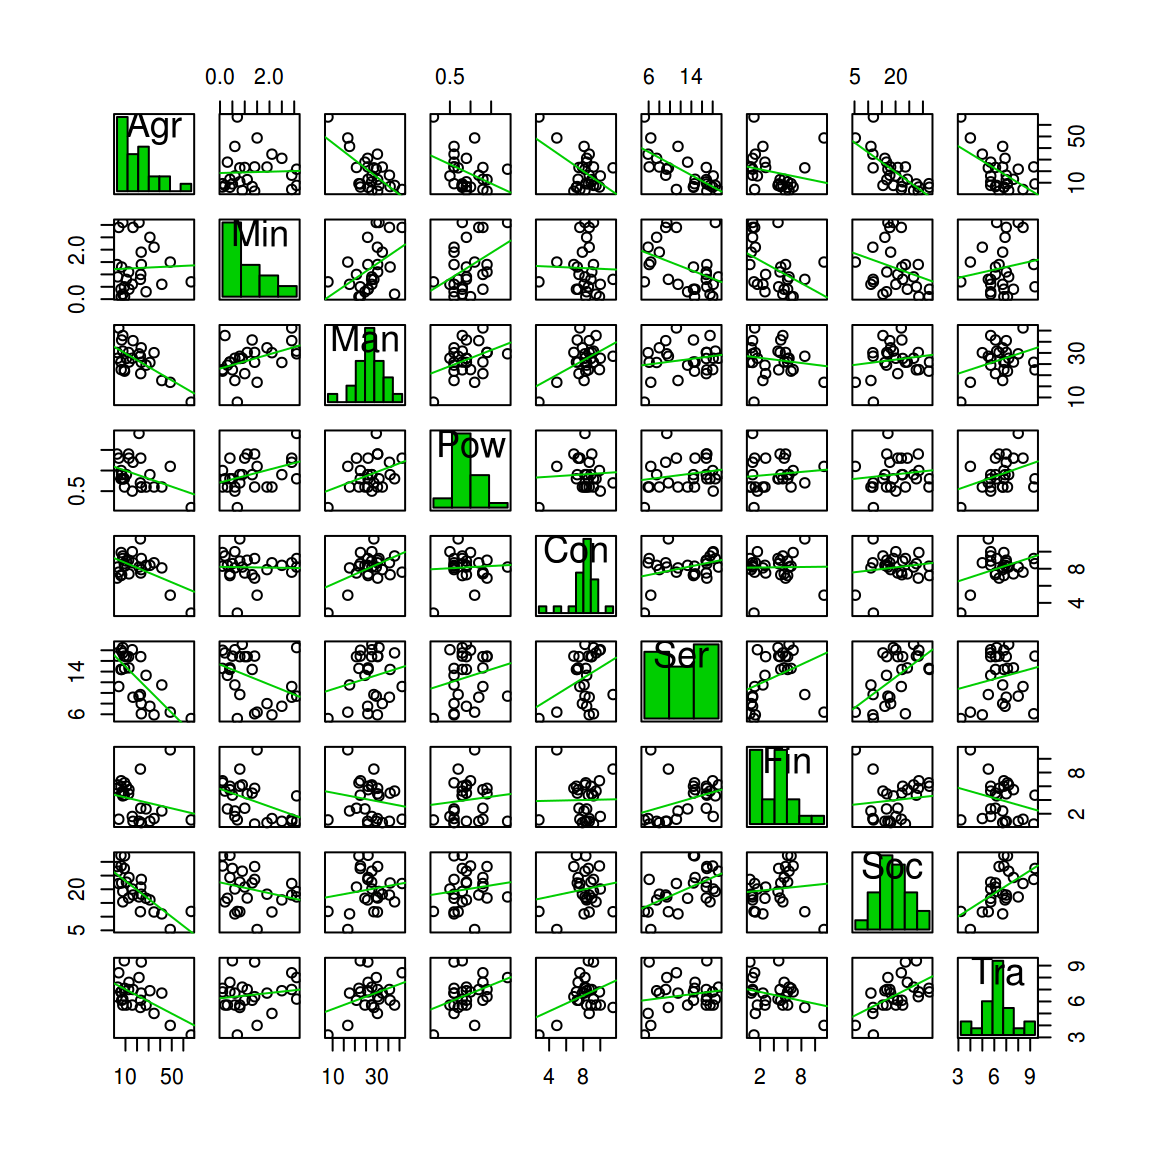
\includegraphics[width=0.7\linewidth]{Machine-Learning_files/figure-latex/unnamed-chunk-113-1} \end{center}

We definitely need a way of visualizing and quantifying the relations
between variables for a moderate to large amount of variables. PCA will
be a handy way. Recall what PCA does:

\begin{enumerate}
\def\labelenumi{\arabic{enumi}.}
\tightlist
\item
  Takes the data for the variables \(X_1,\ldots,X_p\).
\item
  Using this data, looks for new variables
  \(\text{PC}_1,\ldots \text{PC}_p\) such that:

  \begin{itemize}
  \tightlist
  \item
    \(\text{PC}_j\) is a \textbf{linear combination} of
    \(X_1,\ldots,X_k\), \(1\leq j\leq p\). This is,
    \(\text{PC}_j=a_{1j}X_1+a_{2j}X_2+\ldots+a_{pj}X_p\).
  \item
    \(\text{PC}_1,\ldots \text{PC}_p\) are \textbf{sorted decreasingly
    in terms of variance}. Hence \(\text{PC}_j\) has more variance than
    \(\text{PC}_{j+1}\), \(1\leq j\leq p-1\),
  \item
    \(\text{PC}_{j_1}\) and \(\text{PC}_{j_2}\) are
    \textbf{uncorrelated}, for \(j_1\neq j_2\).
  \item
    \(\text{PC}_1,\ldots \text{PC}_p\) have the \textbf{same
    information}, measured in terms of \textbf{total variance}, as
    \(X_1,\ldots,X_p\).
  \end{itemize}
\item
  Produces three key objects:

  \begin{itemize}
  \tightlist
  \item
    \textbf{Variances of the PCs}. They are sorted decreasingly and give
    an idea of which PCs are contain most of the information of the data
    (the ones with more variance).
  \item
    \textbf{Weights of the variables in the PCs}. They give the
    interpretation of the PCs in terms of the original variables, as
    they are the coefficients of the linear combination. The weights of
    the variables \(X_1,\ldots,X_p\) on the PC\(_j\),
    \(a_{1j},\ldots,a_{pj}\), are normalized:
    \(a_{1j}^2+\ldots+a_{pj}^2=1\), \(j=1,\ldots,p\). In \texttt{R},
    they are called \texttt{loadings}.
  \item
    \textbf{Scores of the data in the PCs}: this is the data with
    \(\text{PC}_1,\ldots \text{PC}_p\) variables instead of
    \(X_1,\ldots,X_p\). The \textbf{scores are uncorrelated}. Useful for
    knowing which PCs have more effect on a certain observation.
  \end{itemize}
\end{enumerate}

Hence, PCA rearranges our variables in an information-equivalent, but
more convenient, layout where the variables are \textbf{sorted according
to the ammount of information they are able to explain}. From this
position, the next step is clear: \textbf{stick only with a limited
number of PCs such that they explain most of the information} (e.g.,
70\% of the total variance) and do \emph{dimension reduction}. The
effectiveness of PCA in practice varies from the structure present in
the dataset. For example, in the case of highly dependent data, it could
explain more than the 90\% of variability of a dataset with tens of
variables with just two PCs.

Let's see how to compute a full PCA in \texttt{R}.

\begin{Shaded}
\begin{Highlighting}[]
\CommentTok{# The main function - use cor = TRUE to avoid scale distortions}
\NormalTok{pca <-}\StringTok{ }\KeywordTok{princomp}\NormalTok{(eurojob, }\DataTypeTok{cor =} \OtherTok{TRUE}\NormalTok{)}

\CommentTok{# What is inside?}
\KeywordTok{str}\NormalTok{(pca)}
\CommentTok{#ans> List of 7}
\CommentTok{#ans>  $ sdev    : Named num [1:9] 1.867 1.46 1.048 0.997 0.737 ...}
\CommentTok{#ans>   ..- attr(*, "names")= chr [1:9] "Comp.1" "Comp.2" "Comp.3" "Comp.4" ...}
\CommentTok{#ans>  $ loadings: loadings [1:9, 1:9] -0.52379 -0.00132 0.3475 0.25572 0.32518 ...}
\CommentTok{#ans>   ..- attr(*, "dimnames")=List of 2}
\CommentTok{#ans>   .. ..$ : chr [1:9] "Agr" "Min" "Man" "Pow" ...}
\CommentTok{#ans>   .. ..$ : chr [1:9] "Comp.1" "Comp.2" "Comp.3" "Comp.4" ...}
\CommentTok{#ans>  $ center  : Named num [1:9] 19.131 1.254 27.008 0.908 8.165 ...}
\CommentTok{#ans>   ..- attr(*, "names")= chr [1:9] "Agr" "Min" "Man" "Pow" ...}
\CommentTok{#ans>  $ scale   : Named num [1:9] 15.245 0.951 6.872 0.369 1.614 ...}
\CommentTok{#ans>   ..- attr(*, "names")= chr [1:9] "Agr" "Min" "Man" "Pow" ...}
\CommentTok{#ans>  $ n.obs   : int 26}
\CommentTok{#ans>  $ scores  : num [1:26, 1:9] 1.71 0.953 0.755 0.853 -0.104 ...}
\CommentTok{#ans>   ..- attr(*, "dimnames")=List of 2}
\CommentTok{#ans>   .. ..$ : chr [1:26] "Belgium" "Denmark" "France" "WGerm" ...}
\CommentTok{#ans>   .. ..$ : chr [1:9] "Comp.1" "Comp.2" "Comp.3" "Comp.4" ...}
\CommentTok{#ans>  $ call    : language princomp(x = eurojob, cor = TRUE)}
\CommentTok{#ans>  - attr(*, "class")= chr "princomp"}

\CommentTok{# The standard deviation of each PC}
\NormalTok{pca$sdev}
\CommentTok{#ans>  Comp.1  Comp.2  Comp.3  Comp.4  Comp.5  Comp.6  Comp.7  Comp.8  Comp.9 }
\CommentTok{#ans> 1.86739 1.45951 1.04831 0.99724 0.73703 0.61922 0.47514 0.36985 0.00675}

\CommentTok{# Weights: the expression of the original variables in the PCs}
\CommentTok{# E.g. Agr = -0.524 * PC1 + 0.213 * PC5 - 0.152 * PC6 + 0.806 * PC9}
\CommentTok{# And also: PC1 = -0.524 * Agr + 0.347 * Man + 0256 * Pow + 0.325 * Con + ...}
\CommentTok{# (Because the matrix is orthogonal, so the transpose is the inverse)}
\NormalTok{pca$loadings}
\CommentTok{#ans> }
\CommentTok{#ans> Loadings:}
\CommentTok{#ans>     Comp.1 Comp.2 Comp.3 Comp.4 Comp.5 Comp.6 Comp.7 Comp.8 Comp.9}
\CommentTok{#ans> Agr -0.524                       0.213 -0.153                0.806}
\CommentTok{#ans> Min        -0.618 -0.201        -0.164  0.101  0.726              }
\CommentTok{#ans> Man  0.347 -0.355 -0.150  0.346 -0.385  0.288 -0.479  0.126  0.366}
\CommentTok{#ans> Pow  0.256 -0.261 -0.561 -0.393  0.295 -0.357 -0.256 -0.341       }
\CommentTok{#ans> Con  0.325         0.153  0.668  0.472 -0.130  0.221 -0.356       }
\CommentTok{#ans> Ser  0.379  0.350 -0.115        -0.284 -0.615  0.229  0.388  0.238}
\CommentTok{#ans> Fin         0.454 -0.587         0.280  0.526  0.187  0.174  0.145}
\CommentTok{#ans> Soc  0.387  0.222  0.312 -0.412 -0.220  0.263  0.191 -0.506  0.351}
\CommentTok{#ans> Tra  0.367 -0.203  0.375 -0.314  0.513  0.124         0.545       }
\CommentTok{#ans> }
\CommentTok{#ans>                Comp.1 Comp.2 Comp.3 Comp.4 Comp.5 Comp.6 Comp.7 Comp.8}
\CommentTok{#ans> SS loadings     1.000  1.000  1.000  1.000  1.000  1.000  1.000  1.000}
\CommentTok{#ans> Proportion Var  0.111  0.111  0.111  0.111  0.111  0.111  0.111  0.111}
\CommentTok{#ans> Cumulative Var  0.111  0.222  0.333  0.444  0.556  0.667  0.778  0.889}
\CommentTok{#ans>                Comp.9}
\CommentTok{#ans> SS loadings     1.000}
\CommentTok{#ans> Proportion Var  0.111}
\CommentTok{#ans> Cumulative Var  1.000}

\CommentTok{# Scores of the data on the PCs: how is the data reexpressed into PCs}
\KeywordTok{head}\NormalTok{(pca$scores, }\DecValTok{10}\NormalTok{)}
\CommentTok{#ans>         Comp.1  Comp.2  Comp.3  Comp.4  Comp.5  Comp.6  Comp.7 Comp.8}
\CommentTok{#ans> Belgium  1.710  1.2218 -0.1148 -0.3395 -0.3245  0.0473  0.3401  0.403}
\CommentTok{#ans> Denmark  0.953  2.1278  0.9507 -0.5939  0.1027  0.8273  0.3029 -0.352}
\CommentTok{#ans> France   0.755  1.1212 -0.4980  0.5003 -0.2997 -0.1158  0.1855 -0.266}
\CommentTok{#ans> WGerm    0.853  0.0114 -0.5795  0.1105 -1.1652  0.6181 -0.4446  0.194}
\CommentTok{#ans> Ireland -0.104  0.4140 -0.3840 -0.9267  0.0152 -1.4242  0.0370 -0.334}
\CommentTok{#ans> Italy    0.375  0.7695  1.0606  1.4772 -0.6452 -1.0021  0.1418 -0.130}
\CommentTok{#ans> Luxem    1.059 -0.7558 -0.6515  0.8352 -0.8659 -0.2188  1.6942  0.547}
\CommentTok{#ans> Nether   1.688  2.0048  0.0637  0.0235  0.6352 -0.2120  0.3034 -0.591}
\CommentTok{#ans> UK       1.630  0.3731 -1.1409 -1.2669 -0.8129  0.0361 -0.0413 -0.349}
\CommentTok{#ans> Austria  1.176 -0.1431 -1.0434  0.1577  0.5210 -0.8019 -0.4150  0.215}
\CommentTok{#ans>            Comp.9}
\CommentTok{#ans> Belgium -0.001090}
\CommentTok{#ans> Denmark  0.015619}
\CommentTok{#ans> France  -0.000507}
\CommentTok{#ans> WGerm   -0.006539}
\CommentTok{#ans> Ireland  0.010879}
\CommentTok{#ans> Italy    0.005602}
\CommentTok{#ans> Luxem    0.003453}
\CommentTok{#ans> Nether  -0.010931}
\CommentTok{#ans> UK      -0.005478}
\CommentTok{#ans> Austria -0.002816}

\CommentTok{# Scatterplot matrix of the scores - they are uncorrelated!}
\KeywordTok{scatterplotMatrix}\NormalTok{(pca$scores, }\DataTypeTok{reg.line =} \NormalTok{lm, }\DataTypeTok{smooth =} \OtherTok{FALSE}\NormalTok{, }\DataTypeTok{spread =} \OtherTok{FALSE}\NormalTok{,}
                  \DataTypeTok{span =} \FloatTok{0.5}\NormalTok{, }\DataTypeTok{ellipse =} \OtherTok{FALSE}\NormalTok{, }\DataTypeTok{levels =} \KeywordTok{c}\NormalTok{(.}\DecValTok{5}\NormalTok{, .}\DecValTok{9}\NormalTok{), }\DataTypeTok{id.n =} \DecValTok{0}\NormalTok{,}
                  \DataTypeTok{diagonal =} \StringTok{'histogram'}\NormalTok{)}
\end{Highlighting}
\end{Shaded}

\begin{center}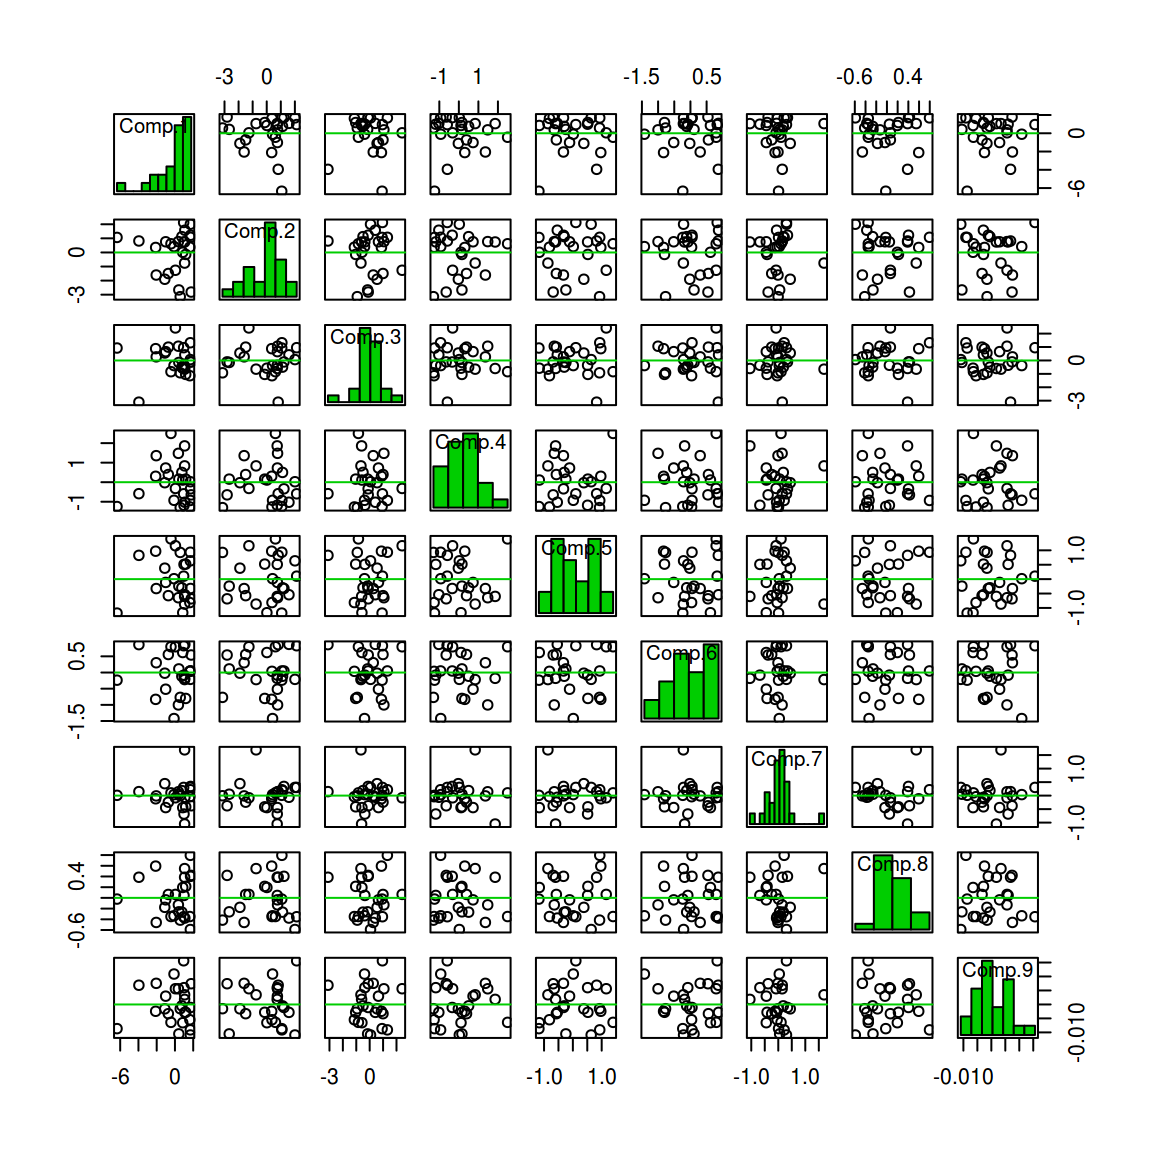
\includegraphics[width=0.7\linewidth]{Machine-Learning_files/figure-latex/unnamed-chunk-114-1} \end{center}

\begin{Shaded}
\begin{Highlighting}[]

\CommentTok{# Means of the variables - before PCA the variables are centered}
\NormalTok{pca$center}
\CommentTok{#ans>    Agr    Min    Man    Pow    Con    Ser    Fin    Soc    Tra }
\CommentTok{#ans> 19.131  1.254 27.008  0.908  8.165 12.958  4.000 20.023  6.546}

\CommentTok{# Rescalation done to each variable}
\CommentTok{# - if cor = FALSE (default), a vector of ones}
\CommentTok{# - if cor = TRUE, a vector with the standard deviations of the variables}
\NormalTok{pca$scale}
\CommentTok{#ans>    Agr    Min    Man    Pow    Con    Ser    Fin    Soc    Tra }
\CommentTok{#ans> 15.245  0.951  6.872  0.369  1.614  4.486  2.752  6.697  1.364}

\CommentTok{# Summary of the importance of components - the third row is key}
\KeywordTok{summary}\NormalTok{(pca)}
\CommentTok{#ans> Importance of components:}
\CommentTok{#ans>                        Comp.1 Comp.2 Comp.3 Comp.4 Comp.5 Comp.6 Comp.7}
\CommentTok{#ans> Standard deviation      1.867  1.460  1.048  0.997 0.7370 0.6192 0.4751}
\CommentTok{#ans> Proportion of Variance  0.387  0.237  0.122  0.110 0.0604 0.0426 0.0251}
\CommentTok{#ans> Cumulative Proportion   0.387  0.624  0.746  0.857 0.9171 0.9597 0.9848}
\CommentTok{#ans>                        Comp.8   Comp.9}
\CommentTok{#ans> Standard deviation     0.3699 6.75e-03}
\CommentTok{#ans> Proportion of Variance 0.0152 5.07e-06}
\CommentTok{#ans> Cumulative Proportion  1.0000 1.00e+00}

\CommentTok{# Scree plot - the variance of each component}
\KeywordTok{plot}\NormalTok{(pca)}
\end{Highlighting}
\end{Shaded}

\begin{center}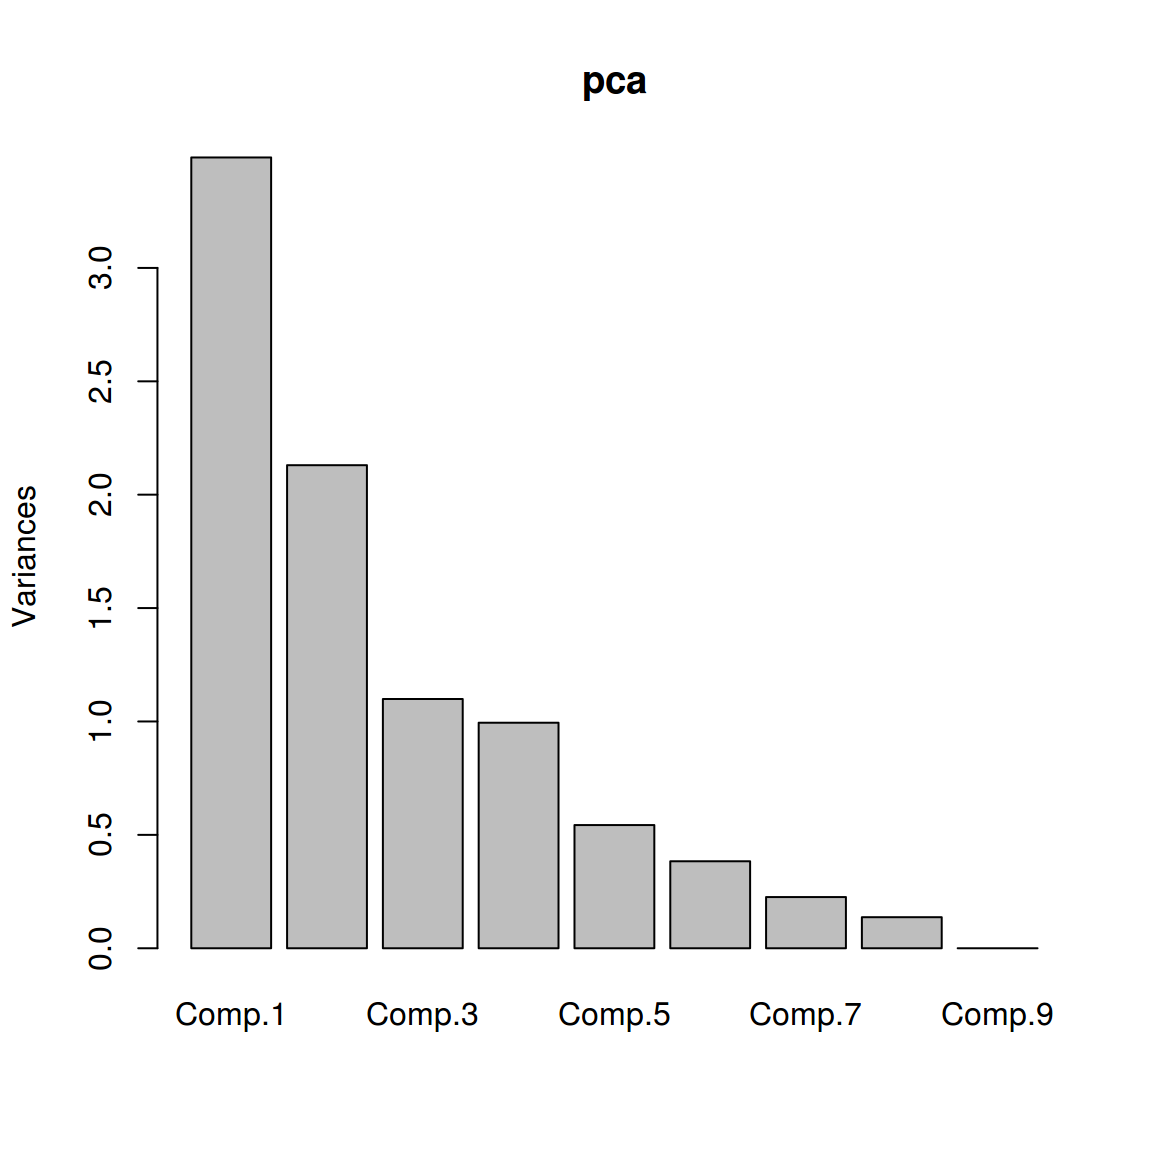
\includegraphics[width=0.7\linewidth]{Machine-Learning_files/figure-latex/unnamed-chunk-114-2} \end{center}

\begin{Shaded}
\begin{Highlighting}[]

\CommentTok{# With connected lines - useful for looking for the "elbow"}
\KeywordTok{plot}\NormalTok{(pca, }\DataTypeTok{type =} \StringTok{"l"}\NormalTok{)}
\end{Highlighting}
\end{Shaded}

\begin{center}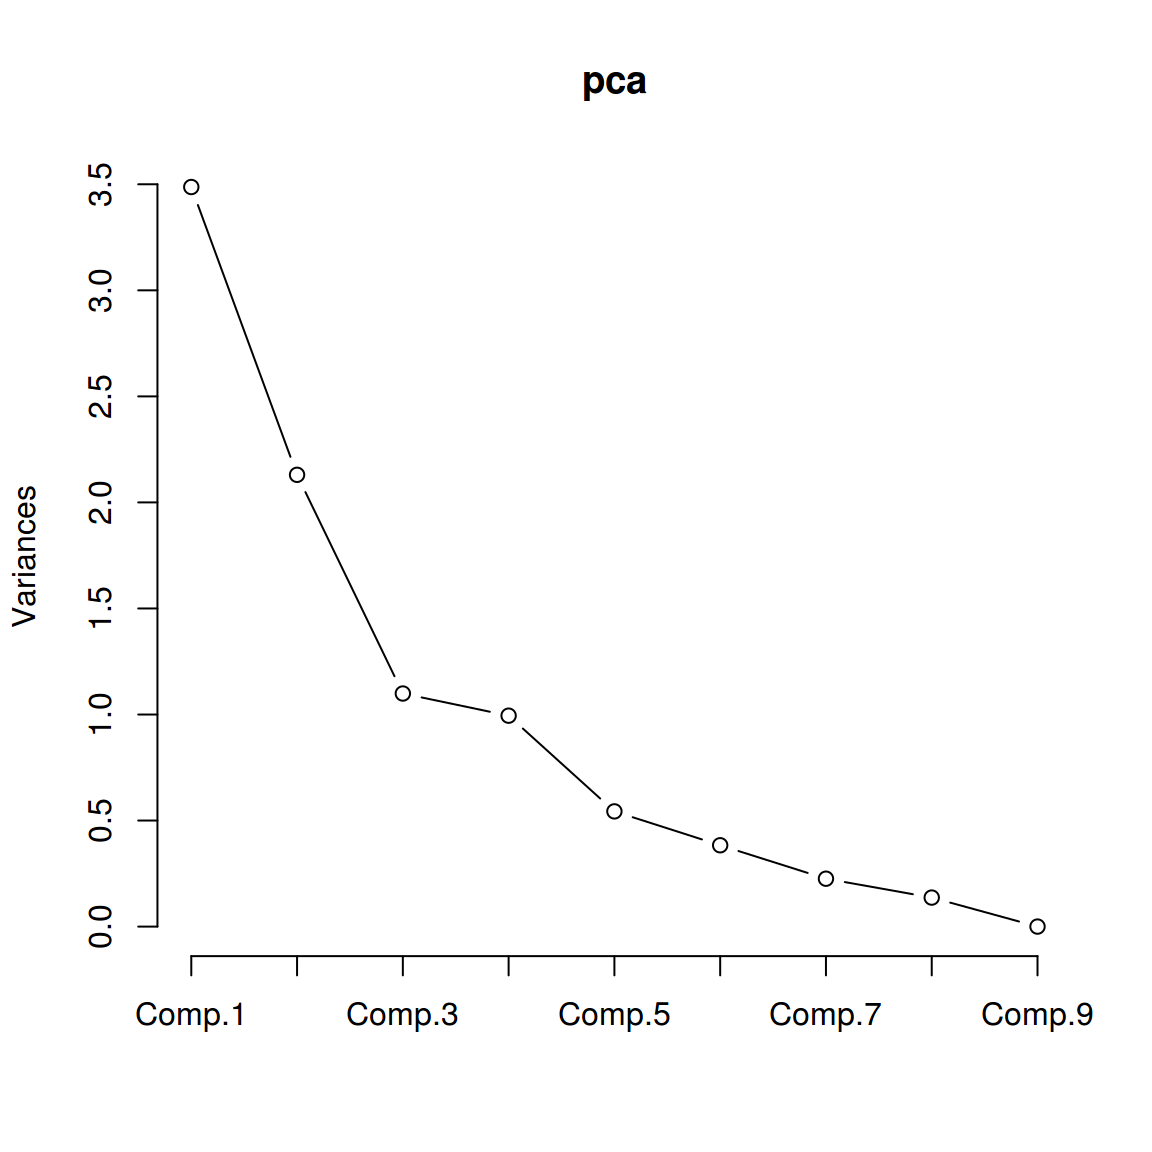
\includegraphics[width=0.7\linewidth]{Machine-Learning_files/figure-latex/unnamed-chunk-114-3} \end{center}

\begin{Shaded}
\begin{Highlighting}[]

\CommentTok{# PC1 and PC2}
\NormalTok{pca$loadings[, }\DecValTok{1}\NormalTok{:}\DecValTok{2}\NormalTok{]}
\CommentTok{#ans>       Comp.1  Comp.2}
\CommentTok{#ans> Agr -0.52379 -0.0536}
\CommentTok{#ans> Min -0.00132 -0.6178}
\CommentTok{#ans> Man  0.34750 -0.3551}
\CommentTok{#ans> Pow  0.25572 -0.2611}
\CommentTok{#ans> Con  0.32518 -0.0513}
\CommentTok{#ans> Ser  0.37892  0.3502}
\CommentTok{#ans> Fin  0.07437  0.4537}
\CommentTok{#ans> Soc  0.38741  0.2215}
\CommentTok{#ans> Tra  0.36682 -0.2026}
\end{Highlighting}
\end{Shaded}

\begin{rmdinsight}
PCA produces \textbf{uncorrelated} variables from the original set
\(X_1,\ldots,X_p\). This implies that:

\begin{itemize}
\tightlist
\item
  The PCs are uncorrelated, \textbf{but not independent} (uncorrelated
  does not imply independent).
\item
  An uncorrelated or independent variable in \(X_1,\ldots,X_p\) will get
  a PC only associated to it. In the extreme case where all the
  \(X_1,\ldots,X_p\) are uncorrelated, these coincide with the PCs (up
  to sign flips).
\end{itemize}
\end{rmdinsight}

Based on the weights of the variables on the PCs, we can extract the
following interpretation:

\begin{itemize}
\tightlist
\item
  PC1 is roughly a linear combination of \texttt{Agr}, with
  \emph{negative} weight, and (\texttt{Man}, \texttt{Pow}, \texttt{Con},
  \texttt{Ser}, \texttt{Soc}, \texttt{Tra}), with \emph{positive}
  weights. So it can be interpreted as an \emph{indicator} of the kind
  of economy of the country: agricultural (negative values) or
  industrial (positive values).
\item
  PC2 has \emph{negative} weights on (\texttt{Min}, \texttt{Man},
  \texttt{Pow}, \texttt{Tra}) and \emph{positive} weights in
  (\texttt{Ser}, \texttt{Fin}, \texttt{Soc}). It can be interpreted as
  the contrast between relatively large or small service sectors. So it
  tends to be negative in communist countries and positive in capitalist
  countries.
\end{itemize}

\begin{rmdtip}
The interpretation of the PCs involves inspecting the weights and
interpreting the linear combination of the original variables, which
might be separating between two clear characteristics of the data
\end{rmdtip}

To conclude, let's see how we can represent our original data into a
plot called \emph{biplot} that summarizes all the analysis for two PCs.

\begin{Shaded}
\begin{Highlighting}[]
\CommentTok{# Biplot - plot together the scores for PC1 and PC2 and the}
\CommentTok{# variables expressed in terms of PC1 and PC2}
\KeywordTok{biplot}\NormalTok{(pca)}
\end{Highlighting}
\end{Shaded}

\begin{center}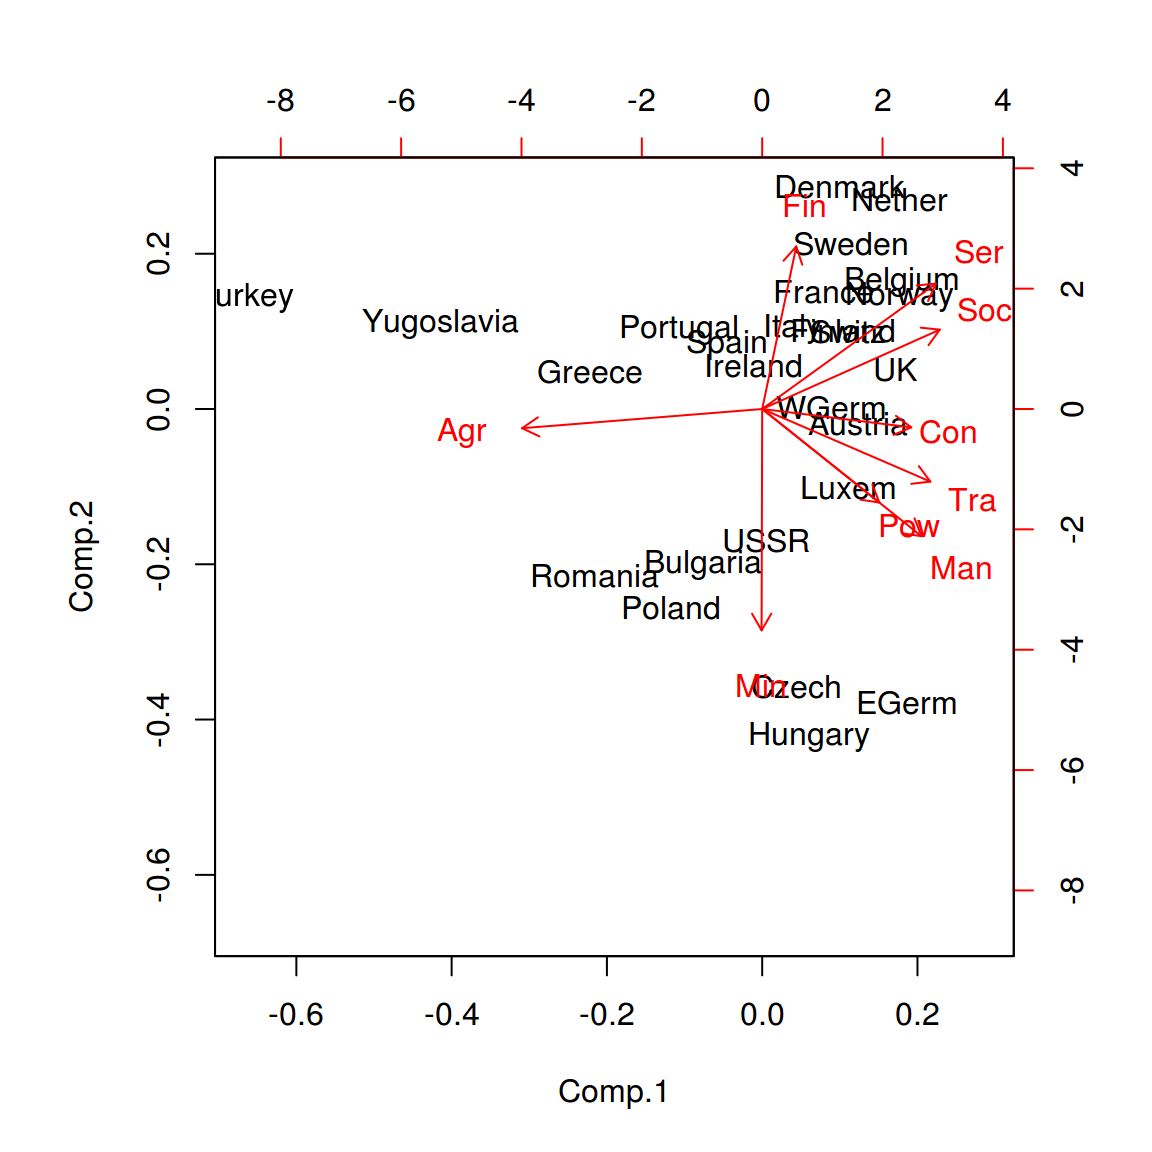
\includegraphics[width=0.9\linewidth]{Machine-Learning_files/figure-latex/unnamed-chunk-117-1} \end{center}

◼

\chapter*{PW 6}\label{pw-6}
\addcontentsline{toc}{chapter}{PW 6}

\section*{The Iris Dataset}\label{the-iris-dataset}
\addcontentsline{toc}{section}{The Iris Dataset}

The iris dataset contains measurements for 150 iris flowers from three
different species.

The three classes in the Iris dataset are:

\begin{enumerate}
\def\labelenumi{\arabic{enumi}.}
\tightlist
\item
  \emph{Iris-setosa} (\(n_1=50\))
\item
  \emph{Iris-versicolor} (\(n_2=50\))
\item
  \emph{Iris-virginica} (\(n_3=50\))
\end{enumerate}

And the four features in Iris dataset are:

\begin{enumerate}
\def\labelenumi{\arabic{enumi}.}
\tightlist
\item
  \emph{sepal length} in cm
\item
  \emph{sepal width} in cm
\item
  \emph{petal length} in cm
\item
  \emph{petal width} in cm
\end{enumerate}

\begin{figure}[htbp]
\centering
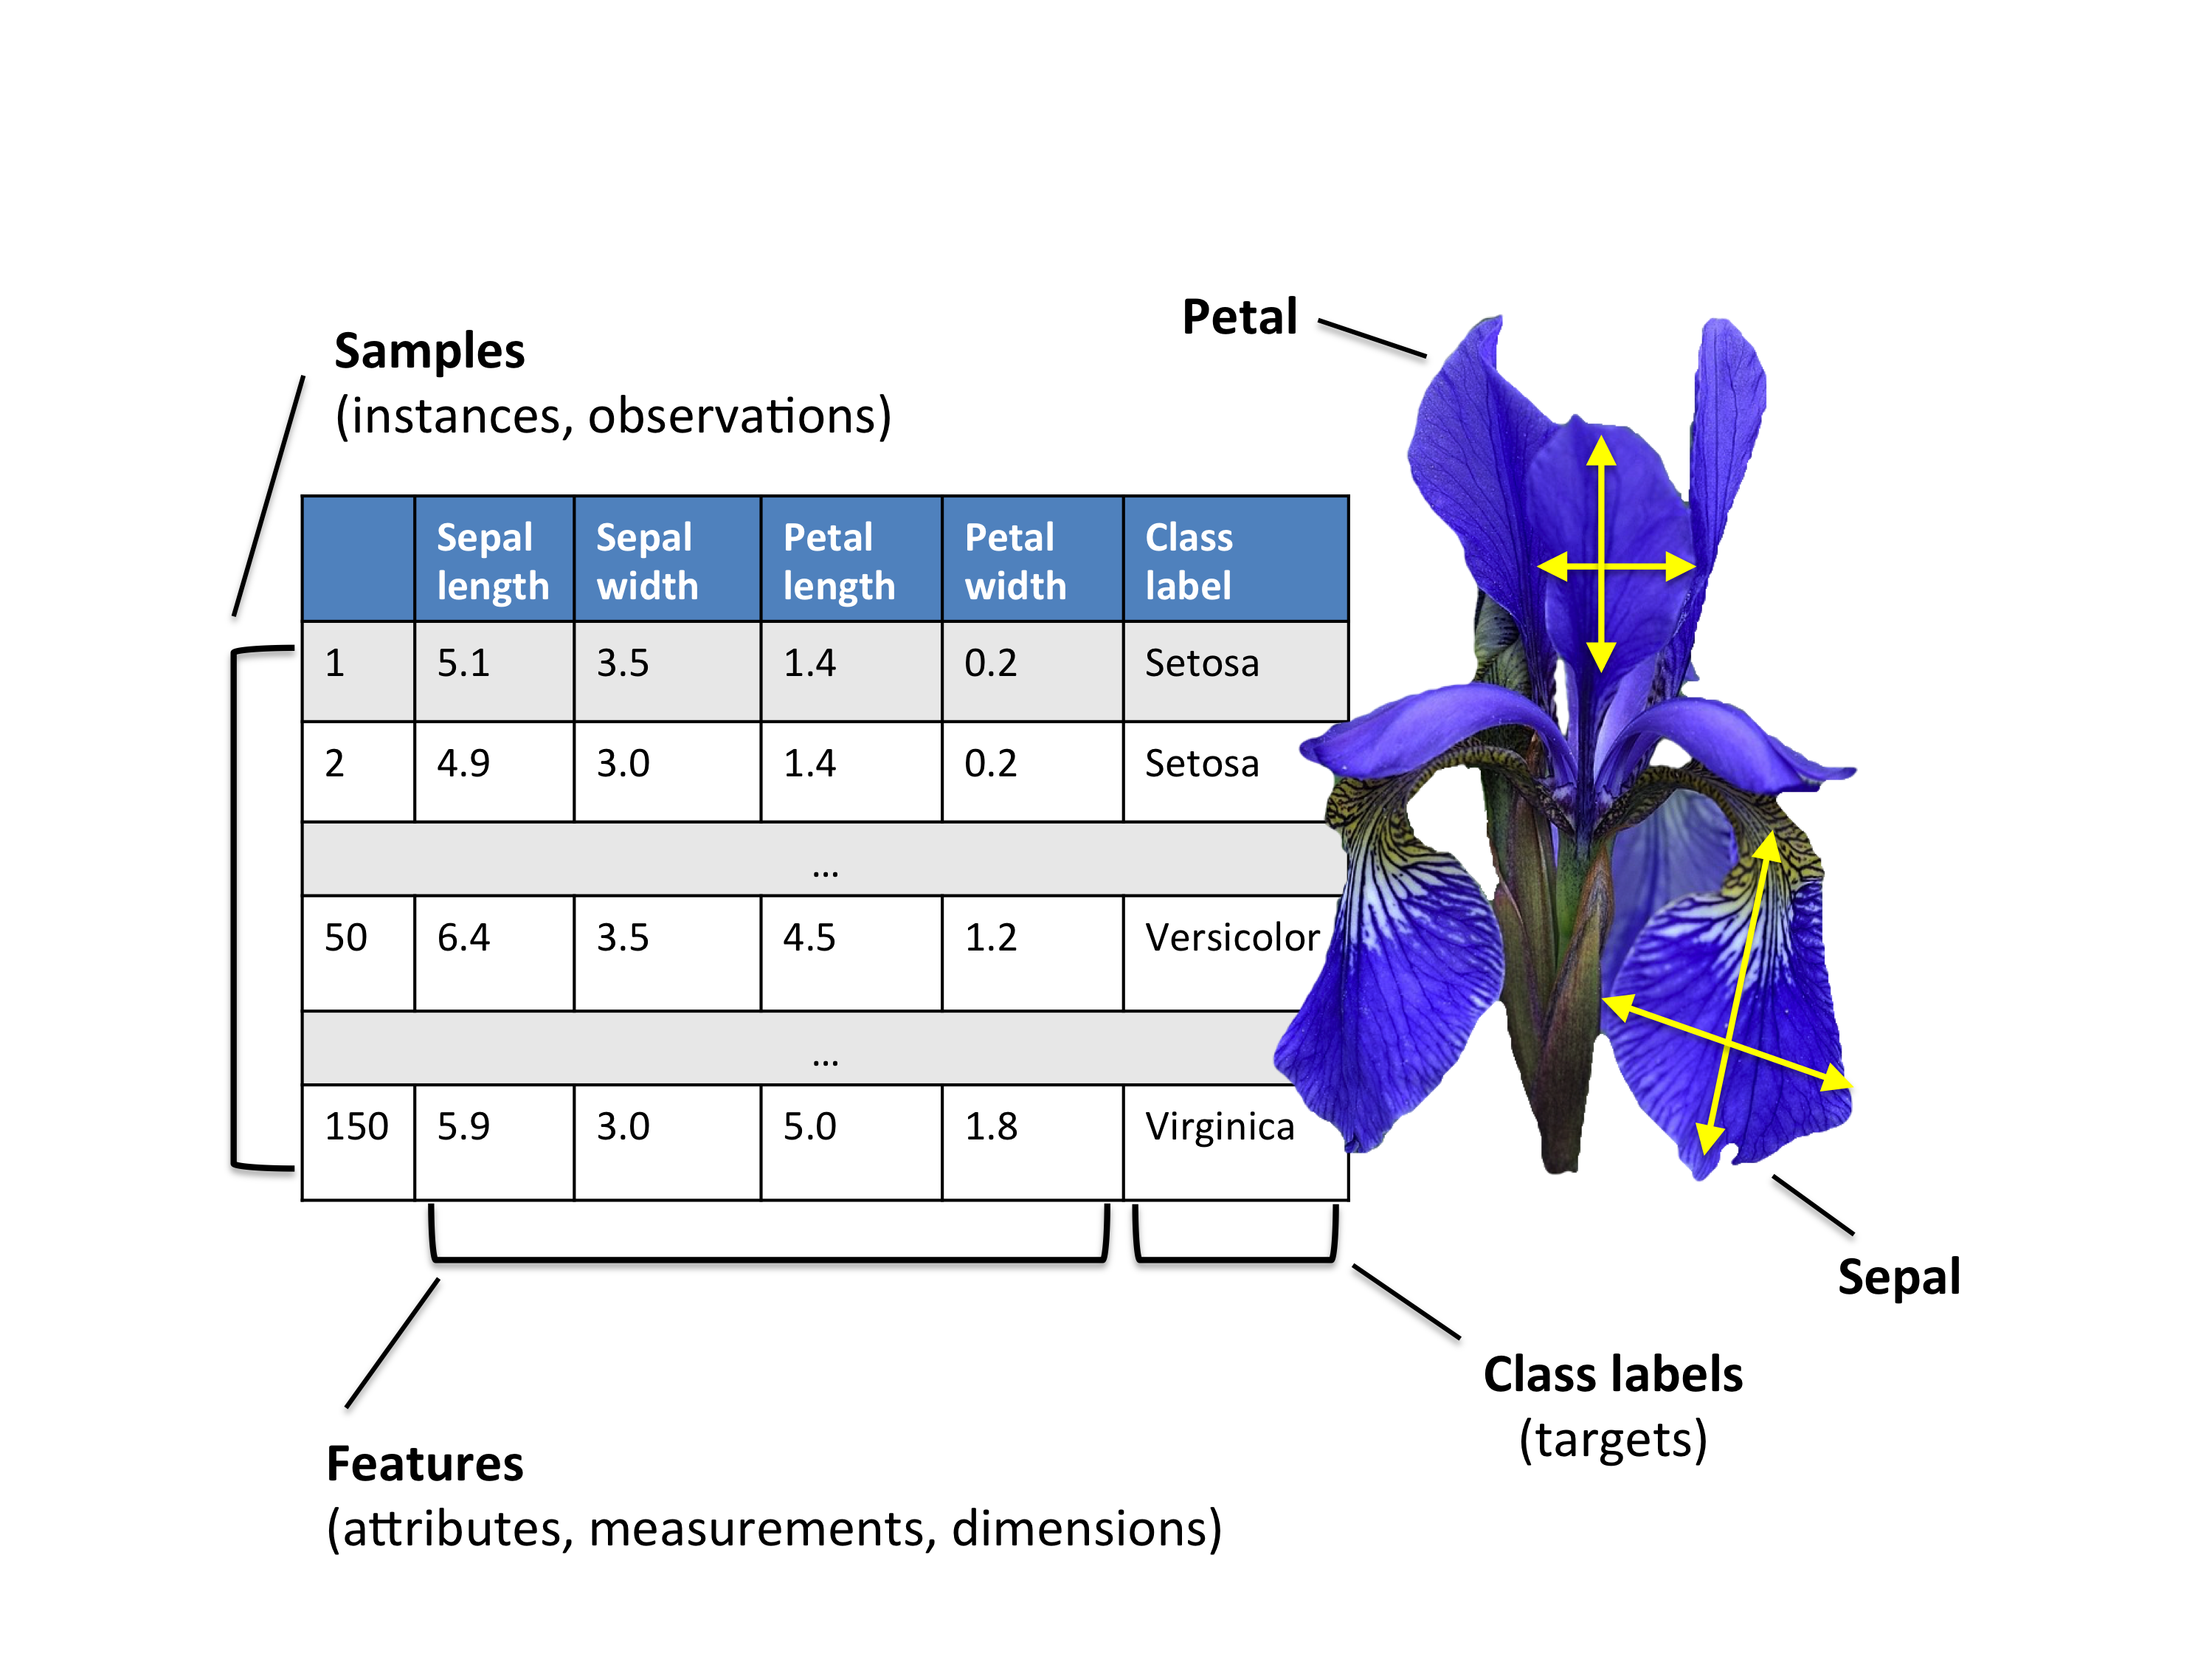
\includegraphics{img/iris.png}
\caption{}
\end{figure}

\section*{Building the PCA approach}\label{building-the-pca-approach}
\addcontentsline{toc}{section}{Building the PCA approach}

\begin{rmdtip}
\textbf{Summary of the PCA Approach}:

\begin{itemize}
\tightlist
\item
  Standardize the data.
\item
  Obtain the Eigenvectors and Eigenvalues from the covariance matrix or
  correlation matrix.
\item
  Sort eigenvalues in descending order and choose the \(k\) eigenvectors
  that correspond to the \(k\) largest eigenvalues, where \(k\) is the
  number of dimensions of the new feature subspace (\(k \le p\)).
\item
  Construct the projection matrix \(\mathbf{A}\) from the selected \(k\)
  eigenvectors.
\item
  Transform the original dataset \(X\) via \(\mathbf{A}\) to obtain a
  \(k\)-dimensional feature subspace \(\mathbf{Y}\).
\end{itemize}
\end{rmdtip}

\subsection*{Data pre-processing}\label{data-pre-processing}
\addcontentsline{toc}{subsection}{Data pre-processing}

\textbf{1.} Download the iris dataset from \faTable  here and import it
into \texttt{R}.

\textbf{2.} Show the last 5 rows of the iris dataset.

\textbf{Exploratory analysis}

\textbf{3.} To explore how the 3 different flower classes are
distributed along the 4 different features, visualize them via
histograms.

\begin{Shaded}
\begin{Highlighting}[]
\CommentTok{# load ggplot2, install it if needed}
\KeywordTok{library}\NormalTok{(ggplot2)}

\CommentTok{# histogram of sepal_length}
\KeywordTok{ggplot}\NormalTok{(iris, }\KeywordTok{aes}\NormalTok{(}\DataTypeTok{x=}\NormalTok{sepal_length, }\DataTypeTok{fill=}\NormalTok{class)) +}
\StringTok{  }\KeywordTok{geom_histogram}\NormalTok{(}\DataTypeTok{binwidth=}\NormalTok{.}\DecValTok{2}\NormalTok{, }\DataTypeTok{alpha=}\NormalTok{.}\DecValTok{5}\NormalTok{)}
\CommentTok{# histogram of sepal_width}
\KeywordTok{ggplot}\NormalTok{(iris, }\KeywordTok{aes}\NormalTok{(}\DataTypeTok{x=}\NormalTok{sepal_width, }\DataTypeTok{fill=}\NormalTok{class)) +}
\StringTok{  }\KeywordTok{geom_histogram}\NormalTok{(}\DataTypeTok{binwidth=}\NormalTok{.}\DecValTok{2}\NormalTok{, }\DataTypeTok{alpha=}\NormalTok{.}\DecValTok{5}\NormalTok{)}
\CommentTok{# histogram of petal_length}
\KeywordTok{ggplot}\NormalTok{(iris, }\KeywordTok{aes}\NormalTok{(}\DataTypeTok{x=}\NormalTok{petal_length, }\DataTypeTok{fill=}\NormalTok{class)) +}
\StringTok{  }\KeywordTok{geom_histogram}\NormalTok{(}\DataTypeTok{binwidth=}\NormalTok{.}\DecValTok{2}\NormalTok{, }\DataTypeTok{alpha=}\NormalTok{.}\DecValTok{5}\NormalTok{)}
\CommentTok{# histogram of petal_width}
\KeywordTok{ggplot}\NormalTok{(iris, }\KeywordTok{aes}\NormalTok{(}\DataTypeTok{x=}\NormalTok{petal_width, }\DataTypeTok{fill=}\NormalTok{class)) +}
\StringTok{  }\KeywordTok{geom_histogram}\NormalTok{(}\DataTypeTok{binwidth=}\NormalTok{.}\DecValTok{2}\NormalTok{, }\DataTypeTok{alpha=}\NormalTok{.}\DecValTok{5}\NormalTok{)}
\end{Highlighting}
\end{Shaded}

\textbf{4.} Compare the means and the quartiles of the 3 different
flower classes for the 4 different features (Plot 4 boxplots into the
same figure).

\textbf{5.} Split the iris dataset into data \(X\) and class labels
\(y\).

\begin{rmdinsight}
The iris dataset is now stored in form of a \(150 \times 4\) matrix
where the columns are the different features, and every row represents a
separate flower sample. Each sample row \(X^i\) can be pictured as a
4-dimensional vector

\[ (X^i)^T = \begin{pmatrix} X_1^i \\ X_2^i \\ X_3^i \\ X_4^i \end{pmatrix}
= \begin{pmatrix} \text{sepal length} \\ \text{sepal width} \\\text{petal length} \\ \text{petal width} \end{pmatrix}\]
\end{rmdinsight}

\subsection*{Eigendecomposition - Computing Eigenvectors and
Eigenvalues}\label{eigendecomposition---computing-eigenvectors-and-eigenvalues}
\addcontentsline{toc}{subsection}{Eigendecomposition - Computing
Eigenvectors and Eigenvalues}

\begin{rmdinsight}
The eigenvectors and eigenvalues of a covariance (or correlation) matrix
represent the ``core'' of a PCA: The eigenvectors (principal components)
determine the directions of the new feature space, and the eigenvalues
determine their magnitude. In other words, the eigenvalues explain the
variance of the data along the new feature axes.
\end{rmdinsight}

\textbf{Standardizing}

\textbf{6.} Scale the 4 features. Store the scaled matrix into a new one
(for example, name it \texttt{x\_scaled}).

\textbf{Covariance Matrix}

\textbf{7.} The classic approach to PCA is to perform the
eigendecomposition on the covariance matrix \(\Sigma\), which is a
\(p\times p\) matrix where each element represents the covariance
between two features. Compute the Covariance Matrix of the scaled
features (Print the results).

\begin{rmdtip}
We can summarize the calculation of the covariance matrix via the
following matrix equation:
\[ \Sigma = \frac{1}{n-1} \left( (\mathbf{X} - \mathbf{\bar{X}})^T\;(\mathbf{X} - \mathbf{\bar{X}}) \right) \]
where \(\mathbf{\bar{X}}\) is the mean vector
\(\mathbf{\bar{X}} = \frac{1}{n} \sum\limits_{k=1}^n x_{k}\).

The mean vector is a \(p\)-dimensional vector where each value in this
vector represents the sample mean of a feature column in the dataset.
\end{rmdtip}

\textbf{8.} Perform an eigendecomposition on the covariance matrix.
Compute the Eigenvectors and the Eigenvalues (you can use the
\texttt{eigen()} function). What do you obtain?

\textbf{Correlation Matrix}

\begin{rmdinsight}
Especially, in the field of ``Finance'', the correlation matrix
typically used instead of the covariance matrix. However, the
eigendecomposition of the covariance matrix (if the input data was
standardized) yields the same results as a eigendecomposition on the
correlation matrix, since the correlation matrix can be understood as
the normalized covariance matrix.
\end{rmdinsight}

\textbf{9.} Perform an eigendecomposition of the standardized data based
on the correlation matrix.

\textbf{10.} Perform an eigendecomposition of the raw data based on the
correlation matrix. Compare the obtained results with the previous
question.

\begin{rmdinsight}
We should see that all three approaches yield the same eigenvectors and
eigenvalue pairs:

\begin{itemize}
\tightlist
\item
  Eigendecomposition of the covariance matrix after standardizing the
  data.
\item
  Eigendecomposition of the correlation matrix.
\item
  Eigendecomposition of the correlation matrix after standardizing the
  data.
\end{itemize}
\end{rmdinsight}

\subsection*{Selecting Principal
Components}\label{selecting-principal-components}
\addcontentsline{toc}{subsection}{Selecting Principal Components}

\begin{rmdinsight}
The \texttt{eigen()} function will, by default, sort the eigenvalues in
decreasing order.
\end{rmdinsight}

\textbf{Explained Variance}

\textbf{11.} Calculate the individual explained variation and the
cumulative explained variation of each principal component. Show the
results.

\textbf{12.} Plot the individual explained variation. (scree plot)

\subsection*{Projection Matrix}\label{projection-matrix}
\addcontentsline{toc}{subsection}{Projection Matrix}

\textbf{13.} Construct the projection matrix that will be used to
transform the Iris data onto the new feature subspace.

\begin{rmdtip}
The ``projection matrix'' is basically just a matrix of our concatenated
top \(k\) eigenvectors. Here, the projection matrix \(\mathbf{A}\) is a
\(4 \times 2\)-dimensional matrix.
\end{rmdtip}

\textbf{Projection Onto the New Feature Space}

In this last step we will use the \(4 \times 2\)-dimensional projection
matrix \(\mathbf{A}\) to transform our samples (observations) onto the
new subspace via the equation \(\mathbf{Y}=X \times \mathbf{A}\) where
\(\mathbf{Y}\) is a \(150 \times 2\) matrix of our transformed samples.

\textbf{14.} Compute \(\mathbf{Y}\) (Recall the \(\mathbf{Y}\) is the
matrix of scores, \(\mathbf{A}\) is the matrix of loadings).

\textbf{Visualization}

\textbf{15.} Plot the observations on the new feature space. Name the
axis PC1 and PC2.

\textbf{16.} On the same plot, color the observations (the flowers) with
respect to their flower classes.

\section*{Verifications with
princomp()}\label{verifications-with-princomp}
\addcontentsline{toc}{section}{Verifications with princomp()}

\textbf{17.} Use the \texttt{princomp()} function as explained in
Chapter 6. Compare the first 5 scores obtained using \texttt{princomp()}
with your results above.

\textbf{18.} Plot together the scores for PC1 and PC2 and the variables
expressed in terms of PC1 and PC2 using \texttt{biplot()}.

\textbf{29.} Interpret the results.

◼


\end{document}
